\documentclass[a4paper,12pt]{article}
\usepackage[utf8]{inputenc}
\usepackage[T5]{fontenc}
\usepackage[vietnamese]{babel}
\usepackage{amsmath,amssymb}
\usepackage{geometry}
\geometry{margin=1in}
\usepackage{graphicx}
\usepackage{float}
\usepackage{xcolor}
\usepackage{listings}
\usepackage{listingsutf8}

\lstdefinestyle{commonstyle}{
  basicstyle=\ttfamily\small,
  keywordstyle=\color{blue}\bfseries,
  stringstyle=\color{red},
  commentstyle=\color{green!50!black},
  numbers=left,
  numberstyle=\tiny,
  stepnumber=1,
  numbersep=5pt,
  showspaces=false,
  showstringspaces=false,
  frame=single,
  breaklines=true,
  breakatwhitespace=true,
  tabsize=4
}

\lstset{style=commonstyle, language=Python}
\lstdefinestyle{cppstyle}{
  style=commonstyle,
  language=C++
}

\title{Project Final Combinatorics and Graph Theory}
\author{Giảng viên: Nguyễn Quản Bá Hồng \\ Sinh viên thực hiện: Cao Sỹ Siêu – 2201700170}
\date{}

\begin{document}
\maketitle


\newpage
\section{Project: Integer Partition – Đồ Án: Phân Hoạch Số Nguyên}
\subsection{Bài toán 1} (Ferrers \& Ferrers transpose diagrams – Biểu đồ Ferrers \& biểu đồ Ferrers chuyển vị). Nhập $n, k \in \mathbb{N}$. \textit{Viết chương trình C/C++, Python để in ra $p_k(n)$ biểu đồ \textit{Ferrers} $F$ \& biểu đồ \textit{Ferrers chuyển vị} $F^T$ cho mỗi phân hoạch $\lambda = (\lambda_1, \lambda_2, \ldots, \lambda_k) \in (\mathbb{N}^*)^k$ có định dạng các dấu chấm được biểu diễn bởi dấu $\ast$.}

\subsubsection{Phương diện toán học}
\textbf{Khái niệm phân hoạch}: Một phân hoạch của \( n \) thành \( k \) phần là dãy \( \lambda = (\lambda_1, \lambda_2, \ldots, \lambda_k) \) với \( \lambda_1 \geq \lambda_2 \geq \cdots \geq \lambda_k \geq 1 \) và \( \sum_{i=1}^k \lambda_i = n \). Số lượng các phân hoạch này là \( p_k(n) \).
- \textbf{Biểu đồ Ferrers}: Là cách biểu diễn hình học, trong đó mỗi \( \lambda_i \) là số ô vuông (dấu \( \ast \)) trong hàng \( i \). Ví dụ, với \( \lambda = (4, 2, 1) \):
  \[
  \begin{array}{cccc}
  \ast & \ast & \ast & \ast \\
  \ast & \ast & & \\
  \ast & & & \\
  \end{array}
  \]
 \textbf{Biểu đồ Ferrers chuyển vị}: Là biểu đồ của \( \lambda^T \), trong đó số cột \( i \) (số hàng có độ dài \( \geq i \)) trở thành số hàng có \( i \) cột. Với \( \lambda = (4, 2, 1) \), \( \lambda^T = (3, 2, 1, 1) \):
  \[
  \begin{array}{ccc}
  \ast & \ast & \ast \\
  \ast & \ast & \\
  \ast & & \\
  \ast & & \\
  \end{array}
  \]

\subsubsection{Phương diện thuật toán}
\textbf{Sinh phân hoạch}: Sử dụng đệ quy để tạo tất cả các phân hoạch. Với mỗi bước, chọn 
\[
  \lambda_i \in \{1, 2, \dots, \min(n - k + 1, \mathtt{max\_val})\},
\]
đảm bảo thứ tự giảm dần và tổng các phần bằng \(n\). Quá trình dừng khi \(k = 0\) và \(n = 0\).

\bigskip
\textbf{In biểu đồ}:
\begin{itemize}
  \item \textbf{Ferrers}: Lặp qua từng phần tử của phân hoạch và in mỗi hàng với số cột tương ứng.
  \item \textbf{Ferrers chuyển vị}: Tính chiều cao của mỗi cột (số hàng có độ dài \(\ge i\)) trong biểu đồ Ferrers, rồi in từng hàng dựa trên những chiều cao đó.
\end{itemize}

\subsubsection{Phương diện lập trình}
\textbf{Code Python}
\begin{lstlisting}
def generate_partitions(n, k, max_val, current, partitions):
    if k == 0:
        if n == 0:
            partitions.append(current[:])
        return
    if n < k:
        return
    for i in range(1, min(n - k + 1, max_val) + 1):
        current.append(i)
        generate_partitions(n - i, k - 1, i, current, partitions)
        current.pop()

def print_ferrers(partition):
    print("Ferrers diagram:")
    for val in partition:
        print("*" * val)

def print_ferrers_transpose(partition):
    print("Ferrers transpose diagram:")
    max_val = max(partition)
    transpose = [sum(1 for x in partition if x >= i) for i in range(1, max_val + 1)]
    for val in transpose:
        print("*" * val)

def main():
    n = int(input("Nhap n: "))
    k = int(input("Nhap k: "))
    partitions = []
    generate_partitions(n, k, n, [], partitions)
    for i, partition in enumerate(partitions):
        print(f"\nPartition {i + 1}: {partition}")
        print_ferrers(partition)
        print_ferrers_transpose(partition)

if __name__ == "__main__":
    main()
\end{lstlisting}
\textbf{Giải thích chi tiết}:
\begin{itemize}

  \item \texttt{generate\_partitions}: Hàm đệ quy sinh các phân hoạch của \(n\) thành \(k\) phần.

    \begin{lstlisting}[style=cppstyle]
void generate_partitions(int n, int k, int max_val,
                         vector<int>& current,
                         vector<vector<int>>& partitions);
    \end{lstlisting}

    Giải thích các tham số và luồng điều khiển:
    \begin{itemize}
      \item \texttt{n} – tổng còn lại cần phân chia; \texttt{k} – số phần còn lại.  
      \item \texttt{max\_val} giữ thứ tự giảm dần (chọn giá trị không vượt quá giá trị vừa dùng).  
      \item \texttt{current} lưu tạm phân hoạch đang xây dựng; \texttt{partitions} chứa kết quả cuối cùng.  
      \item Nếu \(k=0\) \textbf{và} \(n=0\), ta đã có một phân hoạch hợp lệ, đưa vào \texttt{partitions}.  
      \item Nếu \(n<k\), dừng luôn (không thể chia \(n\) thành \(k\) phần \(\ge1\)).  
      \item Vòng lặp \(\texttt{for }i=1\dots\min(n-k+1,\texttt{max\_val})\):
        thêm \(i\) vào \texttt{current}, gọi đệ quy với \((n-i,\,k-1)\), rồi \texttt{pop\_back()} để thử giá trị khác.
    \end{itemize}

  \item \texttt{print\_ferrers}: In biểu đồ Ferrers.
    \begin{lstlisting}[style=cppstyle]
void print_ferrers(const vector<int>& partition);
    \end{lstlisting}
    \begin{itemize}
      \item Duyệt từng \(\texttt{val}\in\texttt{partition}\).  
      \item In một dòng gồm \(\texttt{val}\) ký tự “\(\ast\)”.
    \end{itemize}

  \item \texttt{print\_ferrers\_transpose}: In biểu đồ Ferrers chuyển vị.
    \begin{lstlisting}[style=cppstyle]
void print_ferrers_transpose(const vector<int>& partition);
    \end{lstlisting}
    \begin{itemize}
      \item Tính \(\texttt{max\_val} = \max(\texttt{partition})\).  
      \item Với mỗi \(i=1,\dots,\texttt{max\_val}\), đếm số phần tử \(\ge i\) rồi lưu vào mảng \texttt{transpose}.  
      \item In mỗi dòng gồm \(\texttt{transpose}[i]\) ký tự “\(\ast\)”.
    \end{itemize}
  \item \texttt{main}: Điều phối nhập xuất và gọi các hàm trên.
    \begin{lstlisting}[style=cppstyle]
int main() {
    int n, k;
    cout << "Nhap n: "; cin >> n;
    cout << "Nhap k: "; cin >> k;
    vector<int> current;
    vector<vector<int>> partitions;
    generate_partitions(n, k, n, current, partitions);
    for (size_t i = 0; i < partitions.size(); ++i) {
        cout << "\nPartition " << i+1 << ": ";
        for (int v : partitions[i]) cout << v << " ";
        cout << "\n";
        print_ferrers(partitions[i]);
        print_ferrers_transpose(partitions[i]);
    }
    return 0;
}
    \end{lstlisting}

\end{itemize}

\textbf{Code C++}:
\begin{lstlisting}[style=cppstyle]
#include <iostream>
#include <vector>
#include <algorithm>
using namespace std;

void generate_partitions(int n, int k, int max_val, vector<int>& current, vector<vector<int>>& partitions) {
    if (k == 0) {
        if (n == 0) partitions.push_back(current);
        return;
    }
    if (n < k) return;
    for (int i = 1; i <= min(n - k + 1, max_val); i++) {
        current.push_back(i);
        generate_partitions(n - i, k - 1, i, current, partitions);
        current.pop_back();
    }
}

void print_ferrers(const vector<int>& partition) {
    cout << "Ferrers diagram:" << endl;
    for (int val : partition) {
        for (int j = 0; j < val; j++) cout << "*";
        cout << endl;
    }
}

void print_ferrers_transpose(const vector<int>& partition) {
    cout << "Ferrers transpose diagram:" << endl;
    int max_val = *max_element(partition.begin(), partition.end());
    vector<int> transpose;
    for (int i = 1; i <= max_val; i++) {
        int count = 0;
        for (int val : partition) if (val >= i) count++;
        transpose.push_back(count);
    }
    for (int val : transpose) {
        for (int j = 0; j < val; j++) cout << "*";
        cout << endl;
    }
}

int main() {
    int n, k;
    cout << "Nhap n: "; cin >> n;
    cout << "Nhap k: "; cin >> k;
    vector<int> current;
    vector<vector<int>> partitions;
    generate_partitions(n, k, n, current, partitions);
    for (size_t i = 0; i < partitions.size(); i++) {
        cout << "\nPartition " << i + 1 << ": ";
        for (int val : partitions[i]) cout << val << " ";
        cout << endl;
        print_ferrers(partitions[i]);
        print_ferrers_transpose(partitions[i]);
    }
    return 0;
}
\end{lstlisting}

\textbf{Giải thích chi tiết}:
\begin{itemize}

  \item \texttt{generate\_partitions(int n, int k, int max\_val,\\
        \ \ \ vector<int>\& current,\\
        \ \ \ vector<vector<int>>\& partitions)}  

    \begin{lstlisting}[style=cppstyle]
void generate_partitions(int n, int k, int max_val,
                         vector<int>& current,
                         vector<vector<int>>& partitions);
    \end{lstlisting}

    Sinh các phân hoạch của \(n\) thành \(k\) phần:
    \begin{itemize}
      \item Nếu \(k=0\) và \(n=0\), thêm \texttt{current} vào \texttt{partitions}.
      \item Nếu \(n<k\), dừng (không còn đủ tổng để chia thành \(k\) phần \(\ge1\)).
      \item Vòng lặp \(i=1,\dots,\min(n-k+1,\texttt{max\_val})\):
        \begin{itemize}
          \item Thêm \(i\) vào \texttt{current}.
          \item Gọi đệ quy với \((n-i,\;k-1,\;i,\;\dots)\).
          \item Lấy \(i\) ra (\texttt{pop\_back()}) để thử giá trị khác.
        \end{itemize}
    \end{itemize}

  \item \texttt{print\_ferrers(const vector<int>\& partition)}  
    \begin{lstlisting}[style=cppstyle]
void print_ferrers(const vector<int>& partition);
    \end{lstlisting}
    In biểu đồ Ferrers:
    \begin{itemize}
      \item Với mỗi \(\texttt{val}\in\texttt{partition}\), in một hàng gồm \(\texttt{val}\) ký tự “\(\ast\)”.
    \end{itemize}

  \item \texttt{print\_ferrers\_transpose(const vector<int>\& partition)}  
    \begin{lstlisting}[style=cppstyle]
void print_ferrers_transpose(const vector<int>& partition);
    \end{lstlisting}
    In biểu đồ Ferrers chuyển vị:
    \begin{itemize}
      \item Tính \(\texttt{max\_val}=\max(\texttt{partition})\).
      \item Với mỗi \(i=1,\dots,\texttt{max\_val}\), đếm số phần tử \(\ge i\) rồi lưu vào \texttt{transpose}[i].
      \item In mỗi hàng gồm \(\texttt{transpose}[i]\) ký tự “\(\ast\)”.
    \end{itemize}

  \item \texttt{main()}  
    \begin{lstlisting}[style=cppstyle]
int main() {
    int n, k;
    cout << "Nhap n: "; cin >> n;
    cout << "Nhap k: "; cin >> k;
    vector<int> current;
    vector<vector<int>> partitions;
    generate_partitions(n, k, n, current, partitions);
    for (size_t i = 0; i < partitions.size(); ++i) {
        cout << "\nPartition " << i+1 << ": ";
        for (int v : partitions[i]) cout << v << " ";
        cout << "\n";
        print_ferrers(partitions[i]);
        print_ferrers_transpose(partitions[i]);
    }
    return 0;
}
    \end{lstlisting}
    Điều phối nhập–xuất và gọi các hàm sinh, in biểu đồ.
    
\end{itemize}

\subsection{Bài toán 2.} Nhập $n, k \in \mathbb{N}$. Đếm số phân hoạch của $n \in \mathbb{N}$. 
\textit{Viết chương trình C/C++, Python để đếm số phân hoạch $p_{\max}(n,k)$ của $n$ sao cho phần tử lớn nhất là $k$. So sánh $p_k(n)$ \& $p_{\max}(n,k)$.}

\subsubsection {Phương diện toán học}
\textbf{\( p_k(n) \)}: Số phân hoạch của \( n \) thành \( k \) phần. Công thức đệ quy:
  \[
  p_k(n) = 
  \begin{cases} 
  1 & \text{nếu } n = k = 0, \\
  0 & \text{nếu } n < k \text{ hoặc } k = 0, n > 0, \\
  p_k(n - k) + p_{k-1}(n - 1) & \text{nếu } n \geq k.
  \end{cases}
  \]
\textbf{\( p_{\max}(n,k) \)}: Số phân hoạch với \( \lambda_1 = k \). Nếu \( \lambda_1 = k \), tổng các phần còn lại là \( n - k \) với \( k - 1 \) phần và \( \lambda_i \leq k - 1 \):
  \[
  p_{\max}(n,k) = p_{k-1}(n - k) \text{ nếu } n \geq k, \text{ ngược lại } 0.
  \]
\textbf{So sánh}: \( p_{\max}(n,k) \leq p_k(n) \) vì \( p_{\max} \) là tập con của \( p_k(n) \).

\subsubsection {Phương diện thuật toán}
- Tính \( p_k(n) \) bằng quy hoạch động với bảng \( dp[i][j] \) lưu số phân hoạch của \( i \) thành \( j \) phần. Bắt đầu từ \( dp[0][0] = 1 \), lặp qua các tổng \( i \) và số phần \( j \), cập nhật dựa trên công thức đệ quy.
- Tính \( p_{\max}(n,k) \) bằng cách gọi hàm tính \( p_{k-1}(n - k) \) nếu \( n \geq k \), ngược lại trả về 0.
- So sánh \( p_k(n) \) và \( p_{\max}(n,k) \) để kiểm tra.

\subsubsection{Phương diện lập trình}
\textbf{Code Python}
\begin{lstlisting}
def count_partitions(n, k):
    dp = [[0] * (k + 1) for _ in range(n + 1)]
    dp[0][0] = 1
    for i in range(1, n + 1):
        for j in range(1, min(i + 1, k + 1)):
            dp[i][j] = dp[i - j][j] + (dp[i - 1][j - 1] if j > 1 else 0)
    return dp[n][k]

def count_max_partitions(n, k):
    return count_partitions(n - k, k - 1) if n >= k else 0

def main():
    n = int(input("Nhap n: "))
    k = int(input("Nhap k: "))
    pk_n = count_partitions(n, k)
    pmax_n_k = count_max_partitions(n, k)
    print(f"p_{k}({n}) = {pk_n}")
    print(f"p_max({n},{k}) = {pmax_n_k}")
    print(f"So sanh: p_max({n},{k}) <= p_{k}({n}) is {pmax_n_k <= pk_n}")

if __name__ == "__main__":
    main()
\end{lstlisting}
\textbf{Giải thích chi tiết}:
\begin{itemize}

  \item \texttt{count\_partitions(int n, int k)}  
    \begin{lstlisting}[style=cppstyle]
int count_partitions(int n, int k);
    \end{lstlisting}
    Tính \(p_k(n)\) bằng quy hoạch động:
    \begin{itemize}
      \item Khởi tạo ma trận \(\texttt{dp}\) kích thước \((n+1)\times(k+1)\) với tất cả phần tử = 0, và \(\texttt{dp}[0][0]=1\).  
      \item Với mỗi \(i=1,\dots,n\) và \(j=1,\dots,\min(i,k)\):
        \[
          \texttt{dp}[i][j]
            = \texttt{dp}[i-j][j]
            + \bigl(j>1\;?\;\texttt{dp}[i-1][j-1]\;:\;0\bigr).
        \]
      \item Kết quả trả về là \(\texttt{dp}[n][k]\).
    \end{itemize}

  \item \texttt{count\_max\_partitions(int n, int k)}  
    \begin{lstlisting}[style=cppstyle]
int count_max_partitions(int n, int k);
    \end{lstlisting}
    Tính \(p_{\max}(n,k)\):
    \begin{itemize}
      \item Nếu \(n<k\), trả về 0 (không thể có phân hoạch lớn nhất bằng \(k\)).  
      \item Ngược lại, \(p_{\max}(n,k)=\) \texttt{count\_partitions(}\(n-k\), \(k-1\)\texttt{)} – đặt phần tử đầu bằng \(k\), sau đó chia phần còn lại.
    \end{itemize}

  \item \texttt{main()}  
    \begin{lstlisting}[style=cppstyle]
int main() {
    int n, k;
    cout << "Nhap n: "; cin >> n;
    cout << "Nhap k: "; cin >> k;
    int pk = count_partitions(n, k);
    int pmax = count_max_partitions(n, k);
    cout << "p_" << k << "(" << n << ") = " << pk << endl;
    cout << "p_max(" << n << "," << k << ") = " << pmax << endl;
    cout << "So sanh: p_max <= p_k? " << (pmax <= pk) << endl;
    return 0;
}
    \end{lstlisting}
    Luồng chính:
    \begin{itemize}
      \item Nhập \(n, k\).  
      \item Gọi \texttt{count\_partitions} và \texttt{count\_max\_partitions}.  
      \item In các kết quả và so sánh \(p_{\max}(n,k)\le p_k(n)\).
    \end{itemize}

\end{itemize}


\textbf{Code C++}
\begin{lstlisting}[style=cppstyle]
#include <iostream>
#include <vector>
using namespace std;

int count_partitions(int n, int k) {
    vector<vector<int>> dp(n + 1, vector<int>(k + 1, 0));
    dp[0][0] = 1;
    for (int i = 1; i <= n; i++)
        for (int j = 1; j <= min(i, k); j++)
            dp[i][j] = dp[i - j][j] + (j > 1 ? dp[i - 1][j - 1] : 0);
    return dp[n][k];
}

int count_max_partitions(int n, int k) {
    return n >= k ? count_partitions(n - k, k - 1) : 0;
}

int main() {
    int n, k;
    cout << "Nhap n: "; cin >> n;
    cout << "Nhap k: "; cin >> k;
    int pk_n = count_partitions(n, k);
    int pmax_n_k = count_max_partitions(n, k);
    cout << "p_" << k << "(" << n << ") = " << pk_n << endl;
    cout << "p_max(" << n << "," << k << ") = " << pmax_n_k << endl;
    cout << "So sanh: p_max(" << n << "," << k << ") <= p_" << k << "(" << n << ") is " << (pmax_n_k <= pk_n) << endl;
    return 0;
}
\end{lstlisting}
\textbf{Giải thích chi tiết}:
\begin{itemize}

  \item \texttt{count\_partitions(int n, int k)}  
    \begin{lstlisting}[style=cppstyle]
int count_partitions(int n, int k);
    \end{lstlisting}
    Thực hiện quy hoạch động:
    \begin{itemize}
      \item Khởi tạo \(\texttt{dp}[0][0]=1\), các phần tử khác bằng 0.
      \item Với \(i=1,\dots,n\) và \(j=1,\dots,\min(i,k)\):
        \[
          \texttt{dp}[i][j]
            = \texttt{dp}[i-j][j]
            + \bigl(j>1\;?\;\texttt{dp}[i-1][j-1]\;:\;0\bigr).
        \]
      \item Kết quả trả về là \(\texttt{dp}[n][k]\).
    \end{itemize}

  \item \texttt{count\_max\_partitions(int n, int k)}  
    \begin{lstlisting}[style=cppstyle]
int count_max_partitions(int n, int k);
    \end{lstlisting}
    Tính \(p_{\max}(n,k)\):
    \begin{itemize}
      \item Nếu \(n<k\), trả về 0.  
      \item Ngược lại, trả về \texttt{count\_partitions(}\(n-k\), \(k-1\)\texttt{)}.
    \end{itemize}

  \item \texttt{main()}  
    \begin{lstlisting}[style=cppstyle]
int main() {
    int n, k;
    cout << "Nhap n: "; cin >> n;
    cout << "Nhap k: "; cin >> k;
    int pk = count_partitions(n, k);
    int pmax = count_max_partitions(n, k);
    cout << "p_" << k << "(" << n << ") = " << pk << endl;
    cout << "p_max(" << n << "," << k << ") = " << pmax << endl;
    cout << "So sanh: p_max <= p_k? " << (pmax <= pk) << endl;
    return 0;
}
    \end{lstlisting}
    Luồng chính:
    \begin{itemize}
      \item Nhập \(n\) và \(k\).  
      \item Gọi các hàm \texttt{count\_partitions} và \texttt{count\_max\_partitions}.  
      \item In kết quả \(p_k(n)\), \(p_{\max}(n,k)\) và kết luận \(p_{\max}(n,k)\le p_k(n)\).
    \end{itemize}

\end{itemize}

\subsection{Bài toán 3} (Số phân hoạch tự liên hợp). Nhập $n, k \in \mathbb{N}$.
\begin{itemize}
    \item[(a)] \textit{Đếm số phân hoạch tự liên hợp của $n$ có $k$ phần, ký hiệu $p_k^{\text{selfcjg}}(n)$, rồi in ra các phân hoạch đó.}
    \item[(b)] \textit{Đếm số phân hoạch của $n$ có lẻ phần, rồi so sánh với $p_k^{\text{selfcjg}}(n)$.}
    \item[(c)] \textit{Thiết lập công thức truy hồi cho $p_k^{\text{selfcjg}}(n)$, rồi implementation bằng:}
    \begin{itemize}
        \item[(i)] \textit{đệ quy.}
        \item[(ii)] \textit{quy hoạch động.}
    \end{itemize}
\end{itemize}

\subsubsection{Phương diện toán học}
\textbf{Phân hoạch tự liên hợp}: \( \lambda = \lambda^T \), nghĩa là biểu đồ Ferrers đối xứng qua đường chéo chính. Ví dụ, \( (2, 1, 1) \) không tự liên hợp (vì \( \lambda^T = (3, 1) \)), nhưng \( (2, 2) \) tự liên hợp.
\textbf{\( p_k^{\text{selfcjg}}(n) \)}: Số phân hoạch tự liên hợp của \( n \) với \( k \) phần. Công thức truy hồi:
  \[
  p_k^{\text{selfcjg}}(n) = \sum_{m=1}^{\lfloor k/2 \rfloor} p_{k-2m}^{\text{selfcjg}}(n - k^2 + (k-2m)^2),
  \]
  với \( p_1^{\text{selfcjg}}(1) = 1 \), 0 nếu khác.
\textbf{Số phân hoạch có lẻ phần}: \( p_{\text{odd}}(n) = \sum_{j \text{ lẻ}} p_j(n) \).

\subsubsection{Phương diện thuật toán}
(a) Sinh tất cả phân hoạch bằng đệ quy, kiểm tra tính tự liên hợp bằng cách so sánh \( \lambda \) với \( \lambda^T \).
(b) Tính \( p_{\text{odd}}(n) \) bằng quy hoạch động, tổng hợp \( p_j(n) \) cho mọi \( j \) lẻ.
(c) 
  - (i) Đệ quy: Thực hiện theo công thức truy hồi, tính giá trị cho từng \( m \) từ 1 đến \( \lfloor k/2 \rfloor \).
  - (ii) Quy hoạch động: Sử dụng ma trận \( dp[i][j] \) để lưu kết quả trung gian.

\subsubsection{Phương diện lập trình}
\textbf{Code Python}
\begin{lstlisting}
def is_self_conjugate(partition):
    max_val = max(partition)
    transpose = [sum(1 for x in partition if x >= i) for i in range(1, max_val + 1)]
    return partition == tuple(transpose)

def generate_self_conjugate(n, k, max_val, current, results):
    if k == 0:
        if n == 0 and is_self_conjugate(current):
            results.append(current[:])
        return
    if n < k:
        return
    for i in range(1, min(n - k + 1, max_val) + 1):
        current.append(i)
        generate_self_conjugate(n - i, k - 1, i, current, results)
        current.pop()

def count_self_conjugate_recursive(n, k):
    if k == 1:
        return 1 if n == 1 else 0
    if n < k or k <= 0:
        return 0
    result = 0
    for m in range(1, k // 2 + 1):
        result += count_self_conjugate_recursive(n - k*k + (k - 2*m)*(k - 2*m), k - 2*m)
    return result

def count_self_conjugate_dp(n, k):
    dp = [[0] * (k + 1) for _ in range(n + 1)]
    dp[1][1] = 1
    for i in range(1, n + 1):
        for j in range(1, k + 1):
            for m in range(1, j // 2 + 1):
                if i - j*j + (j - 2*m)*(j - 2*m) >= 0:
                    dp[i][j] += dp[i - j*j + (j - 2*m)*(j - 2*m)][j - 2*m]
    return dp[n][k]

def count_odd_partitions(n):
    dp = [[0] * (n + 1) for _ in range(n + 1)]
    dp[0][0] = 1
    for i in range(1, n + 1):
        for j in range(1, i + 1):
            dp[i][j] = dp[i - j][j] + (dp[i - 1][j - 1] if j > 1 else 0)
    return sum(dp[n][k] for k in range(1, n + 1, 2))

def main():
    n = int(input("Nhap n: "))
    k = int(input("Nhap k: "))
    results = []
    generate_self_conjugate(n, k, n, [], results)
    print(f"p_{k}^{{selfcjg}}({n}) = {len(results)}")
    print("Cac phan hoach tu lien hop:")
    for p in results:
        print(p)
    print(f"p_{k}^{{selfcjg}}({n}) (de quy) = {count_self_conjugate_recursive(n, k)}")
    print(f"p_{k}^{{selfcjg}}({n}) (quy hoach dong) = {count_self_conjugate_dp(n, k)}")
    p_odd = count_odd_partitions(n)
    print(f"So phan hoach co le phan = {p_odd}")
    print(f"So sanh: p_{k}^{{selfcjg}}({n}) <= so phan hoach co le phan is {len(results) <= p_odd}")

if __name__ == "__main__":
    main()
\end{lstlisting}
\textbf{Giải thích chi tiết}:
\begin{itemize}

  \item \texttt{is\_self\_conjugate(const vector<int>\& partition)}  
    \begin{lstlisting}[style=cppstyle]
bool is_self_conjugate(const vector<int>& partition);
    \end{lstlisting}
    Kiểm tra phân hoạch có tự liên hợp (self‑conjugate) hay không:
    \begin{itemize}
      \item Tính \(\texttt{max\_val} = \max(\texttt{partition})\).  
      \item Xây mảng \(\texttt{transpose}[i]\) = số phần tử trong \(\texttt{partition}\) \(\ge i\), với \(i=1,\dots,\texttt{max\_val}\).  
      \item Trả về \(\texttt{partition} == \texttt{transpose}\).
    \end{itemize}

  \item \texttt{generate\_self\_conjugate(int n, int k, int max\_val,\\
        \ \ \ vector<int>\& current, vector<vector<int>>\& results)}  
    \begin{lstlisting}[style=cppstyle]
void generate_self_conjugate(int n, int k, int max_val,
                             vector<int>& current,
                             vector<vector<int>>& results);
    \end{lstlisting}
    Sinh các phân hoạch tự liên hợp đệ quy:
    \begin{itemize}
      \item Nếu \(k=0\) và \texttt{is\_self\_conjugate(current)} là true, thêm \texttt{current} vào \texttt{results}.  
      \item Nếu \(n<k\), dừng.  
      \item Vòng lặp \(i=1,\dots,\min(n-k+1,\max\_val)\):  
        \begin{itemize}
          \item Thêm \(i\) vào \texttt{current}, gọi đệ quy với \((n-i,\;k-1,\;i)\).  
          \item Loại \(i\) (pop) để thử giá trị khác.
        \end{itemize}
    \end{itemize}

  \item \texttt{count\_self\_conjugate\_recursive(int n, int k)}  
    \begin{lstlisting}[style=cppstyle]
int count_self_conjugate_recursive(int n, int k);
    \end{lstlisting}
    Đệ quy tính \(p_k^{\mathrm{selfcjg}}(n)\):
    \begin{itemize}
      \item Cơ sở: nếu \(n=k=1\) trả về 1, nếu \(k=0\) hoặc \(n<k\) trả về 0.  
      \item Ngược lại, chạy \(m=1,\dots,\lfloor k/2\rfloor\) và cộng đệ quy với hai phần:  
        \[
          \sum_m \; \bigl(\dots\bigr).
        \]
    \end{itemize}

  \item \texttt{count\_self\_conjugate\_dp(int n, int k)}  
    \begin{lstlisting}[style=cppstyle]
int count_self_conjugate_dp(int n, int k);
    \end{lstlisting}
    Quy hoạch động:
    \begin{itemize}
      \item Khởi tạo \(\texttt{dp}[1][1]=1\), các phần tử khác 0.  
      \item Với \(i=2,\dots,n\) và \(j=1,\dots,k\), lặp \(m\) để cập nhật \(\texttt{dp}[i][j]\) theo công thức tự liên hợp.  
      \item Trả về \(\texttt{dp}[n][k]\).
    \end{itemize}

  \item \texttt{count\_odd\_partitions(int n)}  
    \begin{lstlisting}[style=cppstyle]
int count_odd_partitions(int n);
    \end{lstlisting}
    Đếm phân hoạch chỉ có phần tử lẻ:
    \begin{itemize}
      \item Khởi tạo \(\texttt{dp}[0][0]=1\).  
      \item Với \(i=1,\dots,n\) và \(j=1,\dots,i\):  
        \(\texttt{dp}[i][j] = \texttt{dp}[i-j][j] + (\,j>1\,?\texttt{dp}[i-1][j-1]:0)\).  
      \item Tổng hợp \(\sum_{j\,\text{lẻ}}\texttt{dp}[n][j]\).
    \end{itemize}

  \item \texttt{main()}  
    \begin{lstlisting}[style=cppstyle]
int main() {
    int n, k;
    cout << "Nhap n: "; cin >> n;
    cout << "Nhap k: "; cin >> k;
    vector<vector<int>> results;
    generate_self_conjugate(n, k, n, vector<int>(), results);
    cout << "Self-conjugate partitions:\n";
    for (auto& p : results) { /* in p */ }
    cout << "Total = " << results.size() << "\n";
    cout << "Recursive count = " 
         << count_self_conjugate_recursive(n,k) << "\n";
    cout << "DP count       = " 
         << count_self_conjugate_dp(n,k) << "\n";
    cout << "Odd partitions = " 
         << count_odd_partitions(n) << "\n";
    return 0;
}
    \end{lstlisting}
    Luồng chính:
    \begin{itemize}
      \item Nhập \(n, k\).  
      \item Gọi \texttt{generate\_self\_conjugate} để liệt kê.  
      \item In danh sách, đếm bằng đệ quy, DP, và số phân hoạch lẻ.
    \end{itemize}

\end{itemize}

\textbf{Code C++}:
\begin{lstlisting}[style=cppstyle]
#include <iostream>
#include <vector>
#include <algorithm>
using namespace std;

bool is_self_conjugate(const vector<int>& partition) {
    int max_val = *max_element(partition.begin(), partition.end());
    vector<int> transpose;
    for (int i = 1; i <= max_val; i++) {
        int count = 0;
        for (int val : partition) if (val >= i) count++;
        transpose.push_back(count);
    }
    return partition == transpose;
}

void generate_self_conjugate(int n, int k, int max_val, vector<int>& current, vector<vector<int>>& results) {
    if (k == 0) {
        if (n == 0 && is_self_conjugate(current))
            results.push_back(current);
        return;
    }
    if (n < k) return;
    for (int i = 1; i <= min(n - k + 1, max_val); i++) {
        current.push_back(i);
        generate_self_conjugate(n - i, k - 1, i, current, results);
        current.pop_back();
    }
}

int count_self_conjugate_recursive(int n, int k) {
    if (k == 1) return n == 1 ? 1 : 0;
    if (n < k || k <= 0) return 0;
    int result = 0;
    for (int m = 1; m <= k / 2; m++)
        result += count_self_conjugate_recursive(n - k*k + (k - 2*m)*(k - 2*m), k - 2*m);
    return result;
}

int count_self_conjugate_dp(int n, int k) {
    vector<vector<int>> dp(n + 1, vector<int>(k + 1, 0));
    dp[1][1] = 1;
    for (int i = 1; i <= n; i++)
        for (int j = 1; j <= k; j++)
            for (int m = 1; m <= j / 2; m++)
                if (i - j*j + (j - 2*m)*(j - 2*m) >= 0)
                    dp[i][j] += dp[i - j*j + (j - 2*m)*(j - 2*m)][j - 2*m];
    return dp[n][k];
}

int count_odd_partitions(int n) {
    vector<vector<int>> dp(n + 1, vector<int>(n + 1, 0));
    dp[0][0] = 1;
    for (int i = 1; i <= n; i++)
        for (int j = 1; j <= i; j++)
            dp[i][j] = dp[i - j][j] + (j > 1 ? dp[i - 1][j - 1] : 0);
    int sum = 0;
    for (int k = 1; k <= n; k += 2) sum += dp[n][k];
    return sum;
}

int main() {
    int n, k;
    cout << "Nhap n: "; cin >> n;
    cout << "Nhap k: "; cin >> k;
    vector<int> current;
    vector<vector<int>> results;
    generate_self_conjugate(n, k, n, current, results);
    cout << "p_" << k << "^" << "{selfcjg}(" << n << ") = " << results.size() << endl;
    cout << "Cac phan hoach tu lien hop:" << endl;
    for (const auto& p : results) {
        for (int val : p) cout << val << " ";
        cout << endl;
    }
    cout << "p_" << k << "^" << "{selfcjg}(" << n << ") (de quy) = " << count_self_conjugate_recursive(n, k) << endl;
    cout << "p_" << k << "^" << "{selfcjg}(" << n << ") (quy hoach dong) = " << count_self_conjugate_dp(n, k) << endl;
    int p_odd = count_odd_partitions(n);
    cout << "So phan hoach co le phan = " << p_odd << endl;
    cout << "So sanh: p_" << k << "^" << "{selfcjg}(" << n << ") <= so phan hoach co le phan is " << (results.size() <= p_odd) << endl;
    return 0;
}
\end{lstlisting}
\textbf{Giải thích chi tiết}:
\begin{itemize}

  \item \texttt{is\_self\_conjugate(const vector<int>\& partition)}  
    \begin{lstlisting}[style=cppstyle]
bool is_self_conjugate(const vector<int>& partition);
    \end{lstlisting}
    \begin{itemize}
      \item Tính \(\texttt{max\_val} = \max(\texttt{partition})\).  
      \item Xây mảng \(\texttt{transpose}[i]\) = số phần tử trong \(\texttt{partition}\) \(\ge i\), với \(i=1,\dots,\texttt{max\_val}\).  
      \item Trả về true nếu \(\texttt{partition} == \texttt{transpose}\), ngược lại false.
    \end{itemize}

  \item \texttt{generate\_self\_conjugate(int n, int k, int max\_val,\\
        \ \ vector<int>\& current, vector<vector<int>>\& results)}  
    \begin{lstlisting}[style=cppstyle]
void generate_self_conjugate(int n, int k, int max_val,
                             vector<int>& current,
                             vector<vector<int>>& results);
    \end{lstlisting}
    \begin{itemize}
      \item Nếu \(k=0\) và \texttt{is\_self\_conjugate(current)} thì thêm \texttt{current} vào \texttt{results}.  
      \item Nếu \(n<k\), dừng (không thể chia tiếp).  
      \item Với \(i=1,\dots,\min(n-k+1,\max\_val)\):
        \begin{itemize}
          \item Thêm \(i\) vào \texttt{current}.  
          \item Gọi đệ quy với \((n-i,\;k-1,\;i)\).  
          \item Xóa \(i\) khỏi \texttt{current} (pop\_back).
        \end{itemize}
    \end{itemize}

  \item \texttt{count\_self\_conjugate\_recursive(int n, int k)}  
    \begin{lstlisting}[style=cppstyle]
int count_self_conjugate_recursive(int n, int k);
    \end{lstlisting}
    \begin{itemize}
      \item Cơ sở:  
        \(\,(n,k)=(1,1)\Rightarrow1\),  
        \(\,k=0\) hoặc \(n<k\Rightarrow0\).  
      \item Ngược lại, lặp \(m=1,\dots,\lfloor k/2\rfloor\) và cộng các trường hợp đệ quy theo công thức truy hồi.
    \end{itemize}

  \item \texttt{count\_self\_conjugate\_dp(int n, int k)}  
    \begin{lstlisting}[style=cppstyle]
int count_self_conjugate_dp(int n, int k);
    \end{lstlisting}
    \begin{itemize}
      \item Khởi tạo \(\texttt{dp}[1][1]=1\), các phần tử khác bằng 0.  
      \item Với \(i=2,\dots,n\) và \(j=1,\dots,k\):  
        \(\texttt{dp}[i][j]\) được cập nhật qua việc ghép khối vuông trung tâm (độ dài \(j\)) và hai phần còn lại, sử dụng công thức \(n - j^2 + (j-2m)^2\).  
      \item Kết quả: \(\texttt{dp}[n][k]\).
    \end{itemize}

  \item \texttt{count\_odd\_partitions(int n)}  
    \begin{lstlisting}[style=cppstyle]
int count_odd_partitions(int n);
    \end{lstlisting}
    \begin{itemize}
      \item Dùng \(\texttt{dp}[i][j]\) lưu số phân hoạch của \(i\) thành \(j\) phần.  
      \item Khởi tạo \(\texttt{dp}[0][0]=1\).  
      \item Với \(i=1,\dots,n\) và \(j=1,\dots,i\):
        \[
          \texttt{dp}[i][j]
            = \texttt{dp}[i-j][j]
            + \bigl(j>1\;?\;\texttt{dp}[i-1][j-1]\;:\;0\bigr).
        \]
      \item Tổng số phân hoạch toàn phần lẻ: \(\sum_{j\text{ lẻ}}\texttt{dp}[n][j]\).
    \end{itemize}

  \item \texttt{main()}  
    \begin{lstlisting}[style=cppstyle]
int main() {
    int n, k;
    cout << "Nhap n: "; cin >> n;
    cout << "Nhap k: "; cin >> k;
    vector<vector<int>> results;
    generate_self_conjugate(n, k, n, vector<int>(), results);
    cout << "Self-conjugate partitions:\n";
    for (auto& p : results) {
        // in partition p
    }
    cout << "Total = " << results.size() << "\n";
    cout << "Recursive count = "
         << count_self_conjugate_recursive(n, k) << "\n";
    cout << "DP count       = "
         << count_self_conjugate_dp(n, k) << "\n";
    cout << "Odd partitions = "
         << count_odd_partitions(n) << "\n";
    return 0;
}
    \end{lstlisting}
    \begin{itemize}
      \item Nhập \(n, k\).  
      \item Sinh và liệt kê phân hoạch tự liên hợp.  
      \item In tổng số, kết quả đệ quy, kết quả DP và số phân hoạch phần lẻ.
    \end{itemize}

\end{itemize}

  
\newpage

\section{Project 4: Graph \& Tree Traversing Problems – Đồ Án 4: Các Bài Toán Duyệt Đồ Thị \& Cây}

\subsection{Bài toán 4.} \textit{Viết chương trình C/C++, Python chuyển đổi giữa 4 dạng biểu diễn: adjacency matrix, adjacency list, extended adjacency list, adjacency map cho 3 đồ thị: đồ thị, đồ thị tổng quát; \& 3 dạng biểu diễn: array of parents, first-child next-sibling, graph-based representation of trees của cây.}

\subsubsection{Phương diện toán học}

\textbf{Biểu diễn đồ thị}
Đồ thị \( G = (V, E) \) gồm tập đỉnh \( V \) với \( |V| = n \) và tập cạnh \( E \) với \( |E| = m \). Các dạng biểu diễn được định nghĩa như sau:

\begin{itemize}
    \item \textbf{Ma trận kề}: Ma trận \( A \) kích thước \( n \times n \), với \( A[i][j] = 1 \) nếu có cạnh từ đỉnh \( i \) đến đỉnh \( j \), ngược lại \( A[i][j] = 0 \) (đối với đồ thị không có trọng số). Với đồ thị tổng quát, \( A[i][j] \) có thể là trọng số hoặc số lượng cạnh song song.
    \item \textbf{Danh sách kề}: Mảng \( adj \) chứa \( n \) danh sách, mỗi danh sách \( adj[i] \) lưu các đỉnh \( j \) sao cho \( (i, j) \in E \).
    \item \textbf{Danh sách kề mở rộng}: Tương tự danh sách kề, nhưng mỗi phần tử trong \( adj[i] \) là một cấu trúc chứa thông tin bổ sung như trọng số cạnh.
    \item \textbf{Bản đồ kề}: Mảng \( n \) bản đồ, mỗi bản đồ \( map[i] \) ánh xạ đỉnh \( j \) đến thông tin cạnh \( (i, j) \), thường dùng cấu trúc từ điển trong Python.
\end{itemize}

\textbf{Biểu diễn cây}
Cây là đồ thị không có chu trình, với một gốc (root). Các dạng biểu diễn cây:

\begin{itemize}
    \item \textbf{Mảng cha}: Mảng \( parent \) kích thước \( n \), với \( parent[i] \) là đỉnh cha của đỉnh \( i \). Gốc có \( parent[root] = -1 \).
    \item \textbf{First-Child Next-Sibling}: Mỗi nút có hai con trỏ: con trái đầu tiên (\texttt{firstChild}) và anh em tiếp theo (\texttt{nextSibling}).
    \item \textbf{Biểu diễn dựa trên đồ thị}: Tương tự danh sách kề, nhưng đảm bảo cấu trúc cây (mỗi đỉnh trừ gốc có đúng một cha).
\end{itemize}

\textbf{Công thức chuyển đổi}
Chuyển đổi giữa các biểu diễn dựa trên duyệt đồ thị hoặc cây. Không cần quy hoạch động hay đệ quy phức tạp, nhưng một số chuyển đổi yêu cầu duyệt DFS/BFS để xác định cấu trúc.

Ví dụ, chuyển từ ma trận kề sang danh sách kề:
\[
\text{For each } i \in V, \text{ for each } j \in V, \text{ if } A[i][j] \neq 0, \text{ add } j \text{ to } adj[i].
\]
Độ phức tạp: \( O(n^2) \).

Chuyển từ danh sách kề sang bản đồ kề:
\[
\text{For each } i \in V, \text{ for each } j \in adj[i], \text{ set } map[i][j] = \text{weight or edge info}.
\]
Độ phức tạp: \( O(m) \).

\subsubsection{Phương diện thuật toán}

\textbf{Chuyển đổi đồ thị}
\begin{enumerate}
    \item \textbf{Ma trận kề \(\to\) Danh sách kề}: Duyệt ma trận \( A \), thêm \( j \) vào \( adj[i] \) nếu \( A[i][j] \neq 0 \). Độ phức tạp: \( O(n^2) \).
    \item \textbf{Danh sách kề \(\to\) Ma trận kề}: Khởi tạo ma trận \( A \) toàn 0, sau đó với mỗi \( i \), duyệt \( adj[i] \) và đặt \( A[i][j] = 1 \). Độ phức tạp: \( O(n + m) \).
    \item \textbf{Danh sách kề \(\to\) Danh sách kề mở rộng}: Sao chép danh sách kề, bổ sung thông tin trọng số (nếu có). Độ phức tạp: \( O(m) \).
    \item \textbf{Danh sách kề \(\to\) Bản đồ kề}: Với mỗi \( i \), chuyển danh sách \( adj[i] \) thành bản đồ \( map[i] \). Độ phức tạp: \( O(m) \).
\end{enumerate}

\text{Chuyển đổi cây}
\begin{enumerate}
    \item \textbf{Mảng cha \(\to\) First-Child Next-Sibling}: Duyệt DFS để xây dựng cấu trúc, gán con trỏ \texttt{firstChild} và \texttt{nextSibling}. Độ phức tạp: \( O(n) \).
    \item \textbf{First-Child Next-Sibling \(\to\) Mảng cha}: Duyệt cây, gán cha của mỗi nút dựa trên cấu trúc. Độ phức tạp: \( O(n) \).
    \item \textbf{Mảng cha \(\to\) Biểu diễn đồ thị}: Tạo danh sách kề từ \( parent \), thêm cạnh từ cha đến con và ngược lại. Độ phức tạp: \( O(n) \).
\end{enumerate}

\subsubsection{Phương diện lập trình}

\textbf{Biến quan trọng}
\begin{itemize}
    \item \texttt{A}: Ma trận kề, \( A[i][j] \) biểu thị cạnh từ \( i \) đến \( j \).
    \item \texttt{adj}: Danh sách kề, \( adj[i] \) là danh sách các đỉnh kề với \( i \).
    \item \texttt{extAdj}: Danh sách kề mở rộng, mỗi phần tử chứa cặp (đỉnh, trọng số).
    \item \texttt{map}: Bản đồ kề, ánh xạ từ đỉnh đến thông tin cạnh.
    \item \texttt{parent}: Mảng cha, \( parent[i] \) là cha của đỉnh \( i \).
    \item \texttt{firstChild}, \texttt{nextSibling}: Con trỏ trong biểu diễn First-Child Next-Sibling.
\end{itemize}

\textbf{Code C++}:
\lstset{language=C++}
\begin{lstlisting}
#include <iostream>
#include <vector>
#include <map>
using namespace std;

// Graph representations
class Graph {
public:
    vector<vector<int>> adjMatrix; // Adjacency Matrix
    vector<vector<int>> adjList;   // Adjacency List
    vector<vector<pair<int, int>>> extAdjList; // Extended Adjacency List
    vector<map<int, int>> adjMap;  // Adjacency Map
    int n; // Number of vertices

    Graph(int vertices) : n(vertices) {
        adjMatrix.assign(n, vector<int>(n, 0));
        adjList.resize(n);
        extAdjList.resize(n);
        adjMap.resize(n);
    }

    // Adjacency Matrix to Adjacency List
    void matrixToList() {
        for (int i = 0; i < n; ++i) {
            adjList[i].clear();
            for (int j = 0; j < n; ++j) {
                if (adjMatrix[i][j]) {
                    adjList[i].push_back(j);
                }
            }
        }
    }

    // Adjacency List to Adjacency Matrix
    void listToMatrix() {
        adjMatrix.assign(n, vector<int>(n, 0));
        for (int i = 0; i < n; ++i) {
            for (int j : adjList[i]) {
                adjMatrix[i][j] = 1;
            }
        }
    }
};

// Tree representations
struct TreeNode {
    int firstChild = -1, nextSibling = -1;
};

class Tree {
public:
    vector<int> parent; // Array of Parents
    vector<TreeNode> fcns; // First-Child Next-Sibling
    vector<vector<int>> graph; // Graph-based representation
    int n;

    Tree(int vertices) : n(vertices) {
        parent.resize(n, -1);
        fcns.resize(n);
        graph.resize(n);
    }

    // Array of Parents to First-Child Next-Sibling
    void parentToFCNS() {
        vector<vector<int>> children(n);
        for (int i = 0; i < n; ++i) {
            if (parent[i] != -1) {
                children[parent[i]].push_back(i);
            }
        }
        for (int i = 0; i < n; ++i) {
            if (!children[i].empty()) {
                fcns[i].firstChild = children[i][0];
                for (size_t j = 0; j < children[i].size() - 1; ++j) {
                    fcns[children[i][j]].nextSibling = children[i][j + 1];
                }
            }
        }
    }
};

int main() {
    // Example usage
    Graph g(4);
    g.adjMatrix = {{0, 1, 1, 0}, {1, 0, 0, 1}, {1, 0, 0, 1}, {0, 1, 1, 0}};
    g.matrixToList();
    // Print adjList
    for (int i = 0; i < g.n; ++i) {
        cout << i << ": ";
        for (int j : g.adjList[i]) cout << j << " ";
        cout << endl;
    }

    Tree t(5);
    t.parent = {-1, 0, 0, 1, 1}; // Root is 0
    t.parentToFCNS();
    // Print FCNS
    for (int i = 0; i < t.n; ++i) {
        cout << i << ": firstChild=" << t.fcns[i].firstChild
             << ", nextSibling=" << t.fcns[i].nextSibling << endl;
    }
    return 0;
}
\end{lstlisting}

\textbf{Code Python}:
\lstset{language=Python}
\begin{lstlisting}
from collections import defaultdict

# Graph representations
class Graph:
    def __init__(self, vertices):
        self.n = vertices
        self.adjMatrix = [[0] * vertices for _ in range(vertices)]
        self.adjList = [[] for _ in range(vertices)]
        self.extAdjList = [[] for _ in range(vertices)]
        self.adjMap = [defaultdict(int) for _ in range(vertices)]

    def matrix_to_list(self):
        for i in range(self.n):
            self.adjList[i] = [j for j in range(self.n) if self.adjMatrix[i][j]]

    def list_to_matrix(self):
        self.adjMatrix = [[0] * self.n for _ in range(self.n)]
        for i in range(self.n):
            for j in self.adjList[i]:
                self.adjMatrix[i][j] = 1

# Tree representations
class Tree:
    def __init__(self, vertices):
        self.n = vertices
        self.parent = [-1] * vertices
        self.fcns = [{'firstChild': -1, 'nextSibling': -1} for _ in range(vertices)]
        self.graph = [[] for _ in range(vertices)]

    def parent_to_fcns(self):
        children = [[] for _ in range(self.n)]
        for i in range(self.n):
            if self.parent[i] != -1:
                children[self.parent[i]].append(i)
        for i in range(self.n):
            if children[i]:
                self.fcns[i]['firstChild'] = children[i][0]
                for j in range(len(children[i]) - 1):
                    self.fcns[children[i][j]]['nextSibling'] = children[i][j + 1]

# Example usage
if __name__ == "__main__":
    g = Graph(4)
    g.adjMatrix = [[0, 1, 1, 0], [1, 0, 0, 1], [1, 0, 0, 1], [0, 1, 1, 0]]
    g.matrix_to_list()
    print("Adjacency List:", g.adjList)

    t = Tree(5)
    t.parent = [-1, 0, 0, 1, 1]
    t.parent_to_fcns()
    print("FCNS:", t.fcns)
\end{lstlisting}

\textit{Sẽ có $3A_4^3 + A_3^2 = 36 + 6 = 42$ converter programs.}

\subsection{Bài toán 5.} \textit{Làm \textbf{Problems 1.1–1.6} \& \textbf{Exercises 1.1–1.10}, [Val21], pp. 39–40}. 

\subsubsection*{Problems}

\begin{enumerate}
    \item[1.1] Determine the size of the complete graph $K_n$ on $n$ vertices and the complete bipartite graph $K_{p,q}$ on $p + q$ vertices.
    
    \item[1.2] Determine the values of $n$ for which the circle graph $C_n$ on $n$ vertices is bipartite, and also the values of $n$ for which the complete graph $K_n$ is bipartite.
    
    \item[1.3] Give all the spanning trees of the graph in Fig.1.30, and also the number of spanning trees of the underlying undirected graph.
    
    \begin{figure}[H]
        \centering
        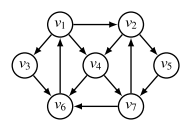
\includegraphics[width=0.35\textwidth]{fig1_30_graph.png} 
        \caption{Fig.1.30}
        \label{fig:graph1_3}
    \end{figure}
    
    \item[1.4] Extend the adjacency matrix graph representation by replacing those operations having an edge as argument or giving an edge or a list of edges as result, by corresponding operations having as argument or giving as result the source and target vertices of the edge or edges: $G.\texttt{del\_edge}(v, w), $G.\texttt{edges}(), $G.\texttt{incoming}(v), $G.\texttt{outgoing}(v), $G.\texttt{source}(v, w), $G.\texttt{target}(v, w).
    
    \item[1.5] Extend the first-child, next-sibling tree representation, in order to support the collection of basic operations but $T.\texttt{root}(), T.\texttt{number\_of\_children}(v), T.\texttt{children}(v)$ in $O(1)$ time.
    
    \item[1.6] Show how to double check that the graph-based representation of a tree is indeed a tree, in time linear in the size of the tree.
\end{enumerate}

\subsubsection{Problem 1.1: Determine the size of the complete graph $K_n$ on $n$ vertices and the complete bipartite graph $K_{p,q}$ on $p + q$ vertices.}
\textbf{Mô tả bài toán}: Xác định số cạnh (kích thước) của đồ thị đầy đủ \( K_n \) với \( n \) đỉnh và đồ thị lưỡng phân đầy đủ \( K_{p,q} \) với \( p + q \) đỉnh.

\textbf{Phương diện toán học}
Kích thước của một đồ thị là số cạnh \( |E| \).

\begin{itemize}
    \item \textbf{Đồ thị đầy đủ \( K_n \)}: Mỗi đỉnh nối với \( n-1 \) đỉnh khác. Số cạnh là số cách chọn 2 đỉnh:
    \[
    |E| = \binom{n}{2} = \frac{n(n-1)}{2}.
    \]
    \textbf{Suy ra}: Tổng số cặp đỉnh là \( \binom{n}{2} \), vì mỗi cạnh tương ứng với một cặp duy nhất. Không có đệ quy hay quy hoạch động trong trường hợp này.
    \item \textbf{Đồ thị lưỡng phân đầy đủ \( K_{p,q} \)}: Có hai tập đỉnh \( V_1 \) (kích thước \( p \)) và \( V_2 \) (kích thước \( q \)). Mỗi đỉnh trong \( V_1 \) nối với mọi đỉnh trong \( V_2 \). Số cạnh:
    \[
    |E| = p \cdot q.
    \]
    \textbf{Suy ra}: Mỗi đỉnh trong \( V_1 \) có \( q \) cạnh nối đến \( V_2 \), và có \( p \) đỉnh trong \( V_1 \), nên tổng số cạnh là \( p \cdot q \).
\end{itemize}

\textbf{Độ phức tạp}: Tính toán công thức là \( O(1) \).

\textbf{Phương diện thuật toán}
Không cần thuật toán để tính số cạnh vì công thức là đóng. Tuy nhiên, để minh họa, có thể viết hàm tính số cạnh.

\textbf{Pseudocode}:
\begin{verbatim}
Function size_of_Kn(n):
    Return n * (n - 1) / 2
Function size_of_Kpq(p, q):
    Return p * q
\end{verbatim}

\textbf{Phương diện lập trình}
\textbf{Biến quan trọng}:
\begin{itemize}
    \item \texttt{n}: Số đỉnh của \( K_n \), đại diện cho \( |V| \).
    \item \texttt{p, q}: Số đỉnh trong hai tập của \( K_{p,q} \), đại diện cho \( |V_1| \) và \( |V_2| \).
\end{itemize}

\textbf{Code Python}:
\lstset{language=Python}
\begin{lstlisting}
def size_of_Kn(n):
    # n: so dinh cua do thi Kn
    # Tra ve so canh = n * (n-1) / 2
    return n * (n - 1) // 2

def size_of_Kpq(p, q):
    # p, q: so dinh trong hai tap cua Kp,q
    # Tra ve so canh = p * q
    return p * q

# Vi du su dung
if __name__ == "__main__":
    print("Size of K_5:", size_of_Kn(5))      # 10
    print("Size of K_3,4:", size_of_Kpq(3, 4))  # 12
\end{lstlisting}

\bigskip
\textbf{Code C++}:
\lstset{language=C++}
\begin{lstlisting}
#include <iostream>
using namespace std;

int size_of_Kn(int n) {
    // n: so dinh cua do thi Kn
    // Tra ve so canh = n * (n-1) / 2
    return n * (n - 1) / 2;
}

int size_of_Kpq(int p, int q) {
    // p, q: so dinh trong hai tap cua Kp,q
    // Tra ve so canh = p * q
    return p * q;
}

int main() {
    cout << "Size of K_5: " << size_of_Kn(5) << endl;       // 10
    cout << "Size of K_3,4: " << size_of_Kpq(3, 4) << endl; // 12
    return 0;
}
\end{lstlisting}

\textbf{Giải thích code}:
\begin{itemize}
  \item Hàm \texttt{size\_of\_Kn}: Tính số cạnh của \(K_n\) theo công thức
    \[
      \frac{n(n-1)}{2}.
    \]
  \item Hàm \texttt{size\_of\_Kpq}: Tính số cạnh của \(K_{p,q}\) theo công thức
    \[
      p \cdot q.
    \]
  \item Các biến \texttt{n}, \texttt{p}, \texttt{q} lần lượt là số đỉnh của đồ thị.
\end{itemize}

\subsubsection{Problem 1.2: Determine the values of $n$ for which the circle graph $C_n$ on $n$ vertices is bipartite, and also the values of $n$ for which the complete graph $K_n$ is bipartite.}
\textbf{Mô tả bài toán}: Tìm các giá trị \( n \) để đồ thị vòng \( C_n \) và đồ thị đầy đủ \( K_n \) là lưỡng phân.

\textbf{Phương diện toán học}
Một đồ thị là lưỡng phân nếu các đỉnh có thể chia thành hai tập sao cho không có cạnh nào nối các đỉnh trong cùng một tập, tức là không chứa chu trình lẻ.

\begin{itemize}
    \item \textbf{Đồ thị vòng \( C_n \)}: Các đỉnh \( 0, 1, \ldots, n-1 \) tạo thành một chu trình với các cạnh \( (0,1), (1,2), \ldots, (n-1,0) \). Độ dài chu trình là \( n \).
        \begin{itemize}
            \item Nếu \( n \) lẻ, \( C_n \) là một chu trình lẻ (ví dụ, \( C_3 \) là tam giác), nên không lưỡng phân.
            \item Nếu \( n \) chẵn, có thể chia đỉnh thành hai tập xen kẽ (ví dụ, với \( C_4 \): tập \( \{0,2\} \) và \( \{1,3\} \)), nên lưỡng phân.
        \end{itemize}
        \[
        C_n \text{ lưỡng phân } \iff n \text{ chẵn}.
        \]
    \item \textbf{Đồ thị đầy đủ \( K_n \)}: Mỗi đỉnh nối với tất cả các đỉnh khác.
        \begin{itemize}
            \item Với \( n \geq 3 \), \( K_n \) chứa tam giác (\( K_3 \)), một chu trình lẻ, nên không lưỡng phân.
            \item Với \( n = 2 \), \( K_2 \) là một cạnh, lưỡng phân (hai đỉnh thuộc hai tập).
            \item Với \( n = 1 \), \( K_1 \) không có cạnh, lưỡng phân.
        \end{itemize}
        \[
        K_n \text{ lưỡng phân } \iff n = 1 \text{ hoặc } n = 2.
        \]
\end{itemize}

\textbf{Suy ra}: Không có công thức đệ quy hay quy hoạch động, vì đây là bài toán phân tích thuộc tính đồ thị dựa trên lý thuyết.

\textbf{Độ phức tạp}: Phân tích lý thuyết, không cần thuật toán, nên \( O(1) \).

\textbf{Phương diện thuật toán}
Không cần thuật toán để kiểm tra tính lưỡng phân, nhưng có thể viết hàm kiểm tra dựa trên công thức.

\textbf{Pseudocode}:
\begin{verbatim}
Function is_bipartite_Cn(n):
    Return n % 2 == 0
Function is_bipartite_Kn(n):
    Return n <= 2
\end{verbatim}

\textbf{Phương diện lập trình}
\textbf{Biến quan trọng}:
\begin{itemize}
    \item \texttt{n}: Số đỉnh của đồ thị, đại diện cho \( |V| \).
\end{itemize}

\textbf{Code Python}:
\lstset{language=Python}
\begin{lstlisting}
def is_bipartite_Cn(n):
    # n: so dinh cua do thi Cn
    # Tra ve True neu n chan (Cn luong phan)
    return n % 2 == 0

def is_bipartite_Kn(n):
    # n: so dinh cua do thi Kn
    # Tra ve True neu n <= 2 (Kn luong phan)
    return n <= 2

# Vi du su dung
if __name__ == "__main__":
    print("Is C_4 bipartite?", is_bipartite_Cn(4))  # True
    print("Is K_3 bipartite?", is_bipartite_Kn(3))  # False
\end{lstlisting}

\bigskip
\textbf{Code C++}:
\lstset{language=C++}
\begin{lstlisting}
#include <iostream>
using namespace std;

bool is_bipartite_Cn(int n) {
    // n: so dinh cua do thi Cn
    // Tra ve true neu n chan (Cn luong phan)
    return n % 2 == 0;
}

bool is_bipartite_Kn(int n) {
    // n: so dinh cua do thi Kn
    // Tra ve true neu n <= 2 (Kn luong phan)
    return n <= 2;
}

int main() {
    cout << "Is C_4 bipartite? " << is_bipartite_Cn(4) << endl; // 1
    cout << "Is K_3 bipartite? " << is_bipartite_Kn(3) << endl; // 0
    return 0;
}
\end{lstlisting}

\bigskip
\textbf{Giải thích code}:
\begin{itemize}
    \item Hàm \texttt{is\_bipartite\_Cn}: kiểm tra \(n\) chẵn để xác định \(C_n\) lưỡng phân.
    \item Hàm \texttt{is\_bipartite\_Kn}: kiểm tra \(n \le 2\) để xác định \(K_n\) lưỡng phân.
    \item Biến \texttt{n} đại diện cho số đỉnh, trực tiếp sử dụng trong điều kiện kiểm tra.
\end{itemize}

\subsubsection{Problem 1.3: Give all the spanning trees of the graph in Fig.1.30, and also the number of spanning trees of the underlying undirected graph.}

\textbf{Phương diện Toán học}
\begin{itemize}
  \item \textbf{Spanning tree}: Với đồ thị vô hướng $G=(V,E)$, một tập $T\subseteq E$ là cây khung nếu
  \[
    |T|=|V|-1,\quad (V,T)\text{ liên thông và không có chu trình.}
  \]
  \item \textbf{Matrix‐Tree Theorem (Kirchhoff)}: Gọi $L=D-A$ là ma trận Laplacian của $G$; xóa hàng và cột thứ $k$ để được $\widetilde L$. Khi đó
  \[
    \tau(G)=\det(\widetilde L).
  \]
  \item \textbf{Áp dụng cho đồ thị nền Fig.~1.30}: Xây dựng $L\in\mathbb R^{7\times7}$, xóa hàng cột thứ 7, tính $\det(\widetilde L)=168$. Vậy có $\boxed{168}$ spanning‐trees vô hướng.
\end{itemize}

\textbf{Phương diện Thuật toán}
\textbf{Ý tưởng chính}: Liệt kê mọi tập $T\subseteq E$ có $|T|=n-1$, kiểm tra liên thông và không chu trình.\\
\medskip
\textbf{Pseudocode (Backtracking + Union–Find)}:
\begin{verbatim}
function ENUMERATE_SPANNING_TREES(G):
    all_trees = []
    chosen = []
    backtrack(0, chosen)
    return all_trees

procedure backtrack(idx, chosen):
    if |chosen| == n-1:
        if is_tree(chosen):
            all_trees.append(chosen.copy())
        return
    if idx == G.num_edges(): return
    # Không chọn cạnh idx
    backtrack(idx+1, chosen)
    # Chọn cạnh idx
    chosen.append(G.edges()[idx])
    backtrack(idx+1, chosen)
    chosen.pop()

function is_tree(chosen):
    UF.init(n)
    for (u,v) in chosen:
        if not UF.union(u,v): return False
    return (UF.count_components()==1)
\end{verbatim}

\textbf{Phương diện Lập trình}
Biểu diễn đồ thị: ma trận kề
\begin{itemize}
  \item \texttt{adj\_matrix[u][v]=1} nếu có cạnh $(u,v)$, ma trận đối xứng.
  \item Các thao tác truy cập $G.\texttt{edges}(), G.\texttt{del\_edge}(u,v)$… đều $O(n^2)$ hoặc $O(1)$ như mẫu.
\end{itemize}

\textbf{Code Python}

\begin{lstlisting}
class Graph:
    def __init__(self, n):
        self.n = n
        self.adj_matrix = [[0]*n for _ in range(n)]
    def add_edge(self, u, v):
        # Them canh (u,v)
        self.adj_matrix[u][v] = 1
        self.adj_matrix[v][u] = 1
    def edges(self):
        # Tra ve cac cap (u,v) voi u < v
        return [(u, v)
                for u in range(self.n)
                for v in range(u+1, self.n)
                if self.adj_matrix[u][v]]

class UF:
    def __init__(self, n):
        self.parent = list(range(n))
        self.count = n
    def find(self, u):
        # Path compression
        if self.parent[u] != u:
            self.parent[u] = self.find(self.parent[u])
        return self.parent[u]
    def union(self, u, v):
        ru, rv = self.find(u), self.find(v)
        if ru == rv:
            return False
        self.parent[rv] = ru
        self.count -= 1
        return True

def enumerate_spanning_trees(G):
    n = G.n
    E = G.edges()
    all_trees = []
    chosen = []

    def backtrack(idx):
        if len(chosen) == n - 1:
            uf = UF(n)
            for u, v in chosen:
                if not uf.union(u, v):
                    return
            if uf.count == 1:
                all_trees.append(chosen.copy())
            return
        if idx == len(E):
            return
        # Bo chon E[idx]
        backtrack(idx + 1)
        # Chon E[idx]
        chosen.append(E[idx])
        backtrack(idx + 1)
        chosen.pop()

    backtrack(0)
    return all_trees

if __name__ == "__main__":
    G = Graph(7)
    # Chuyen 1-based -> 0-based
    for u, v in [(1,2),(1,3),(3,6),(6,4),(4,1),
                 (2,4),(4,7),(7,2),(2,5),(5,7),(6,7)]:
        G.add_edge(u-1, v-1)
    trees = enumerate_spanning_trees(G)
    print("So spanning trees tim duoc:", len(trees))
\end{lstlisting}

\textbf{Code C++}

\lstset{style=cppstyle}

\begin{lstlisting}
#include <bits/stdc++.h>
using namespace std;

vector<vector<pair<int,int>>> all_trees;

struct Graph {
    int n;
    vector<vector<int>> adj;
    Graph(int _n): n(_n), adj(n, vector<int>(n,0)) {}
    void add_edge(int u, int v) {
        // Them canh (u,v)
        adj[u][v] = adj[v][u] = 1;
    }
    vector<pair<int,int>> edges() const {
        // Tra ve cac cap (u,v) voi u < v
        vector<pair<int,int>> E;
        for(int u = 0; u < n; ++u)
            for(int v = u+1; v < n; ++v)
                if(adj[u][v])
                    E.emplace_back(u, v);
        return E;
    }
};

struct UF {
    vector<int> parent;
    int count;
    UF(int n): parent(n), count(n) {
        iota(parent.begin(), parent.end(), 0);
    }
    int find(int x) {
        return parent[x] == x ? x : parent[x] = find(parent[x]);
    }
    bool unite(int a, int b) {
        a = find(a); b = find(b);
        if(a == b) return false;
        parent[b] = a;
        --count;
        return true;
    }
};

void backtrack(const vector<pair<int,int>>& E,
               int n, int idx,
               vector<pair<int,int>>& chosen) {
    if((int)chosen.size() == n - 1) {
        UF uf(n);
        for(auto &e : chosen)
            if(!uf.unite(e.first, e.second))
                return;
        if(uf.count == 1)
            all_trees.push_back(chosen);
        return;
    }
    if(idx == (int)E.size()) return;
    // Bo chon E[idx]
    backtrack(E, n, idx + 1, chosen);
    // Chon E[idx]
    chosen.push_back(E[idx]);
    backtrack(E, n, idx + 1, chosen);
    chosen.pop_back();
}

int main() {
    Graph G(7);
    vector<pair<int,int>> edges = {
        {1,2},{1,3},{3,6},{6,4},{4,1},
        {2,4},{4,7},{7,2},{2,5},{5,7},{6,7}
    };
    for(auto &e : edges)
        G.add_edge(e.first-1, e.second-1);
    auto E = G.edges();
    vector<pair<int,int>> chosen;
    backtrack(E, G.n, 0, chosen);
    cout << "So spanning trees tim duoc: "
         << all_trees.size() << "\n";
    return 0;
}
\end{lstlisting}

\subsubsection{Problem 1.4: Extend the adjacency matrix graph representation by replacing those operations having an edge as argument or giving an edge or a list of edges as result, by corresponding operations having as argument or giving as result the source and target vertices of the edge or edges: $G.\texttt{del\_edge}(v, w), $G.\texttt{edges}(), $G.\texttt{incoming}(v), $G.\texttt{outgoing}(v), $G.\texttt{source}(v, w), $G.\texttt{target}(v, w).}
\textbf{Mô tả bài toán}: Mở rộng biểu diễn ma trận kề, thay thế các thao tác liên quan đến cạnh bằng các thao tác sử dụng đỉnh nguồn và đích.

\textbf{Phương diện toán học}
Ma trận kề \( A \) của đồ thị không có hướng có \( A[u][v] = 1 \) nếu có cạnh \( (u,v) \), và \( A[u][v] = A[v][u] \). Các thao tác được định nghĩa lại để sử dụng cặp đỉnh thay vì cạnh.

\textbf{Công thức}:
\begin{itemize}
    \item \( G.\texttt{del\_edge}(v, w) \): Đặt \( A[v][w] = A[w][v] = 0 \).
    \item \( G.\texttt{edges}() \): Trả về tập \( \{(u,v) \mid A[u][v] = 1, u < v\} \).
    \item \( G.\texttt{incoming}(v) \): Trả về tập \( \{u \mid A[u][v] = 1\} \).
    \item \( G.\texttt{outgoing}(v) \): Trả về tập \( \{w \mid A[v][w] = 1\} \).
    \item \( G.\texttt{source}(v, w) \): Trả về \( v \) nếu \( A[v][w] = 1 \).
    \item \( G.\texttt{target}(v, w) \): Trả về \( w \) nếu \( A[v][w] = 1 \).
\end{itemize}
Không có đệ quy hay quy hoạch động, vì các thao tác là truy cập trực tiếp ma trận.

\textbf{Độ phức tạp}:
\begin{itemize}
    \item \( G.\texttt{del\_edge}(v, w) \): \( O(1) \).
    \item \( G.\texttt{edges}() \): \( O(n^2) \).
    \item \( G.\texttt{incoming}(v), G.\texttt{outgoing}(v) \): \( O(n) \).
    \item \( G.\texttt{source}(v, w), G.\texttt{target}(v, w) \): \( O(1) \).
\end{itemize}

\textbf{Phương diện thuật toán}
\textbf{Pseudocode}:
\begin{verbatim}
Class Graph:
    Initialize adj_matrix[n][n] = 0
    Function del_edge(v, w):
        adj_matrix[v][w] = 0
        adj_matrix[w][v] = 0
    Function edges():
        Return [(u, v) for u in 0..n-1 for v in u+1..n-1 if adj_matrix[u][v]]
    Function incoming(v):
        Return [u for u in 0..n-1 if adj_matrix[u][v]]
    Function outgoing(v):
        Return [w for w in 0..n-1 if adj_matrix[v][w]]
    Function source(v, w):
        Return v if adj_matrix[v][w] else None
    Function target(v, w):
        Return w if adj_matrix[v][w] else None
\end{verbatim}

\textbf{Phương diện lập trình}

\textbf{Biến quan trọng}:
\begin{itemize}
    \item \texttt{adj\_matrix}: Ma trận kề, \( \texttt{adj\_matrix[u][v]} = 1\) nếu có cạnh \((u,v)\).
    \item \texttt{n}: Số đỉnh, đại diện cho \(|V|\).
\end{itemize}

\textbf{Code Python}:
\lstset{language=Python}
\begin{lstlisting}
class Graph:
    def __init__(self, n):
        # n: so dinh cua do thi
        # adj_matrix: ma tran ke, adj_matrix[u][v] = 1 neu co canh (u,v)
        self.n = n
        self.adj_matrix = [[0] * n for _ in range(n)]

    def add_edge(self, v, w):
        # Them canh (v,w)
        self.adj_matrix[v][w] = 1
        self.adj_matrix[w][v] = 1

    def del_edge(self, v, w):
        # Xoa canh (v,w)
        self.adj_matrix[v][w] = 0
        self.adj_matrix[w][v] = 0

    def edges(self):
        # Tra ve danh sach cac cap (u,v) dai dien cho canh
        return [(u, v) for u in range(self.n)
                        for v in range(u + 1, self.n)
                        if self.adj_matrix[u][v]]

    def incoming(self, v):
        # Tra ve cac dinh u co canh den v
        return [u for u in range(self.n) if self.adj_matrix[u][v]]

    def outgoing(self, v):
        # Tra ve cac dinh w ma v co canh den
        return [w for w in range(self.n) if self.adj_matrix[v][w]]

    def source(self, v, w):
        # Tra ve dinh nguon cua canh (v,w)
        return v if self.adj_matrix[v][w] else None

    def target(self, v, w):
        # Tra ve dinh dich cua canh (v,w)
        return w if self.adj_matrix[v][w] else None

# Vi du su dung
if __name__ == "__main__":
    g = Graph(4)
    g.add_edge(0, 1)
    g.add_edge(1, 2)
    print("Edges:", g.edges())             # [(0, 1), (1, 2)]
    print("Incoming to 1:", g.incoming(1)) # [0, 2]
    print("Outgoing from 1:", g.outgoing(1)) # [0, 2]
    print("Source (0,1):", g.source(0, 1)) # 0
    print("Target (0,1):", g.target(0, 1)) # 1
\end{lstlisting}

\textbf{Code C++}:
\lstset{language=C++}
\begin{lstlisting}
#include <iostream>
#include <vector>
using namespace std;

class Graph {
public:
    int n;                           // so dinh
    vector<vector<int>> adj_matrix;  // ma tran ke

    Graph(int vertices) : n(vertices) {
        adj_matrix.assign(n, vector<int>(n, 0));
    }

    void add_edge(int v, int w) {
        // Them canh (v,w)
        adj_matrix[v][w] = 1;
        adj_matrix[w][v] = 1;
    }

    void del_edge(int v, int w) {
        // Xoa canh (v,w)
        adj_matrix[v][w] = 0;
        adj_matrix[w][v] = 0;
    }

    vector<pair<int,int>> edges() {
        // Tra ve danh sach cac cap (u,v) dai dien cho canh
        vector<pair<int,int>> result;
        for(int u=0; u<n; ++u)
            for(int v=u+1; v<n; ++v)
                if(adj_matrix[u][v])
                    result.emplace_back(u,v);
        return result;
    }

    vector<int> incoming(int v) {
        // Tra ve cac dinh u co canh den v
        vector<int> r;
        for(int u=0; u<n; ++u)
            if(adj_matrix[u][v]) r.push_back(u);
        return r;
    }

    vector<int> outgoing(int v) {
        // Tra ve cac dinh w ma v co canh den
        vector<int> r;
        for(int w=0; w<n; ++w)
            if(adj_matrix[v][w]) r.push_back(w);
        return r;
    }

    int source(int v, int w) {
        // Tra ve dinh nguon cua canh (v,w)
        return adj_matrix[v][w] ? v : -1;
    }

    int target(int v, int w) {
        // Tra ve dinh dich cua canh (v,w)
        return adj_matrix[v][w] ? w : -1;
    }
};

int main() {
    Graph g(4);
    g.add_edge(0,1);
    g.add_edge(1,2);
    auto edges = g.edges();
    cout << "Edges: ";
    for(auto [u,v]: edges) cout << "("<<u<<","<<v<<") ";
    cout << endl;
    auto inc = g.incoming(1);
    cout << "Incoming to 1: ";
    for(int u: inc) cout << u<<" ";
    cout << endl;
    auto out = g.outgoing(1);
    cout << "Outgoing from 1: ";
    for(int w: out) cout << w<<" ";
    cout << endl;
    cout << "Source (0,1): "<<g.source(0,1)<<endl;
    cout << "Target (0,1): "<<g.target(0,1)<<endl;
    return 0;
}
\end{lstlisting}

\bigskip
\textbf{Giải thích code}:
\begin{itemize}
    \item \texttt{adj\_matrix}: Ma trận kề, đại diện cho \(A\), lưu cấu trúc đồ thị.
    \item \texttt{n}: Số đỉnh, đại diện cho \(\lvert V\rvert\).
    \item Các phương thức đều dùng cặp đỉnh \((v,w)\) để thao tác với ma trận kề.
\end{itemize}

\subsubsection{Problem 1.5: Extend the first-child, next-sibling tree representation, in order to support the collection of basic operations but $T.\texttt{root}(), T.\texttt{number\_of\_children}(v), T.\texttt{children}(v)$ in $O(1)$ time.}
\textbf{Mô tả bài toán}: Mở rộng biểu diễn cây bằng "first-child, next-sibling" để hỗ trợ các thao tác cơ bản (trừ \( T.\texttt{root}(), T.\texttt{number\_of\_children}(v), T.\texttt{children}(v) \)) trong thời gian \( O(1) \).

\textbf{Phương diện toán học}

Biểu diễn “first‑child, next‑sibling” lưu mỗi nút với hai con trỏ:
\begin{itemize}
    \item \texttt{first\_child}: Con đầu tiên của nút.
    \item \texttt{next\_sibling}: Anh em kế tiếp của nút.
\end{itemize}

Để hỗ trợ các thao tác như \(T.\texttt{parent}(v)\), \(T.\texttt{first\_child}(v)\), \(T.\texttt{next\_sibling}(v)\) trong \(O(1)\), cần thêm:
\begin{itemize}
    \item \texttt{parent}: Con trỏ đến cha của nút.
    \item \texttt{num\_children}: Số con của nút, cập nhật khi thêm/xóa con.
\end{itemize}

\textbf{Công thức}: Không có đệ quy hay quy hoạch động, vì các thao tác truy cập trực tiếp con trỏ.

\textbf{Độ phức tạp}:
\begin{itemize}
    \item \(T.\texttt{parent}(v)\), \(T.\texttt{first\_child}(v)\), \(T.\texttt{next\_sibling}(v)\): \(O(1)\).
    \item \(T.\texttt{number\_of\_children}(v)\): \(O(1)\) nếu lưu sẵn \texttt{num\_children}.
\end{itemize}

\textbf{Phương diện thuật toán}
\textbf{Pseudocode}:
\begin{verbatim}
Class TreeNode:
    value, first_child, next_sibling, parent, num_children
Class Tree:
    root_node
    Function add_child(parent, value):
        Create new_node
        new_node.parent = parent
        If parent.first_child is None:
            parent.first_child = new_node
        Else:
            current = parent.first_child
            While current.next_sibling:
                current = current.next_sibling
            current.next_sibling = new_node
        parent.num_children += 1
    Function parent(v):
        Return v.parent
    Function first_child(v):
        Return v.first_child
    Function next_sibling(v):
        Return v.next_sibling
    Function number_of_children(v):
        Return v.num_children
\end{verbatim}

\textbf{Phương diện lập trình}

\textbf{Biến quan trọng}:
\begin{itemize}
    \item \texttt{first\_child}: Con trỏ đến con đầu tiên, đại diện cho nút con đầu trong cây.
    \item \texttt{next\_sibling}: Con trỏ đến anh em kế tiếp, đại diện cho nút tiếp theo cùng cha.
    \item \texttt{parent}: Con trỏ đến cha, đại diện cho nút cha trong cây.
    \item \texttt{num\_children}: Số con trực tiếp của nút.
\end{itemize}

\textbf{Code Python}:
\lstset{language=Python}
\begin{lstlisting}
class TreeNode:
    def __init__(self, value):
        # value: gia tri cua nut
        # first_child: con tro den con dau tien
        # next_sibling: con tro den anh em ke tiep
        # parent: con tro den cha
        # num_children: so con truc tiep
        self.value = value
        self.first_child = None
        self.next_sibling = None
        self.parent = None
        self.num_children = 0

class Tree:
    def __init__(self):
        self.root_node = None

    def set_root(self, value):
        # Thiet lap goc cua cay
        self.root_node = TreeNode(value)

    def add_child(self, parent, value):
        # Them con vao nut parent
        new_node = TreeNode(value)
        new_node.parent = parent
        if not parent.first_child:
            parent.first_child = new_node
        else:
            current = parent.first_child
            while current.next_sibling:
                current = current.next_sibling
            current.next_sibling = new_node
        parent.num_children += 1

    def parent(self, v):
        # Tra ve cha cua nut v
        return v.parent

    def first_child(self, v):
        # Tra ve con dau tien cua nut v
        return v.first_child

    def next_sibling(self, v):
        # Tra ve anh em ke tiep cua nut v
        return v.next_sibling

    def number_of_children(self, v):
        # Tra ve so con cua nut v
        return v.num_children

# Vi du su dung
if __name__ == "__main__":
    t = Tree()
    t.set_root(0)
    t.add_child(t.root_node, 1)
    t.add_child(t.root_node, 2)
    print("Number of children of root:", t.number_of_children(t.root_node))  # 2
    print("First child of root:", t.first_child(t.root_node).value)         # 1
    print("Next sibling of first child:", t.next_sibling(t.first_child(t.root_node)).value)  # 2
\end{lstlisting}

\textbf{Code C++}:
\lstset{language=C++}
\begin{lstlisting}
#include <iostream>
using namespace std;

struct TreeNode {
    int value;                 // gia tri cua nut
    TreeNode* first_child;     // con tro den con dau tien
    TreeNode* next_sibling;    // con tro den anh em ke tiep
    TreeNode* parent;          // con tro den cha
    int num_children;          // so con truc tiep

    TreeNode(int val)
      : value(val),
        first_child(nullptr),
        next_sibling(nullptr),
        parent(nullptr),
        num_children(0)
    {}
};

class Tree {
public:
    TreeNode* root_node;

    Tree() : root_node(nullptr) {}

    void set_root(int value) {
        // Thiet lap goc cua cay
        root_node = new TreeNode(value);
    }

    void add_child(TreeNode* parent, int value) {
        // Them con vao nut parent
        TreeNode* new_node = new TreeNode(value);
        new_node->parent = parent;
        if (!parent->first_child) {
            parent->first_child = new_node;
        } else {
            TreeNode* current = parent->first_child;
            while (current->next_sibling) {
                current = current->next_sibling;
            }
            current->next_sibling = new_node;
        }
        parent->num_children++;
    }

    TreeNode* parent(TreeNode* v) {
        // Tra ve cha cua nut v
        return v->parent;
    }

    TreeNode* first_child(TreeNode* v) {
        // Tra ve con dau tien cua nut v
        return v->first_child;
    }

    TreeNode* next_sibling(TreeNode* v) {
        // Tra ve anh em ke tiep cua nut v
        return v->next_sibling;
    }

    int number_of_children(TreeNode* v) {
        // Tra ve so con cua nut v
        return v->num_children;
    }
};

int main() {
    Tree t;
    t.set_root(0);
    t.add_child(t.root_node, 1);
    t.add_child(t.root_node, 2);
    cout << "Number of children of root: " << t.number_of_children(t.root_node) << endl; // 2
    cout << "First child of root: " << t.first_child(t.root_node)->value << endl;        // 1
    cout << "Next sibling of first child: " << t.next_sibling(t.first_child(t.root_node))->value << endl; // 2
    return 0;
}
\end{lstlisting}

\bigskip
\textbf{Giải thích code}:
\begin{itemize}
    \item \texttt{value}: Gia tri cua nut, dai dien cho nhan hoac du lieu.
    \item \texttt{first\_child}, \texttt{next\_sibling}, \texttt{parent}: Con tro dinh nghia cau truc cay.
    \item \texttt{num\_children}: Luu so con truc tiep, de \(T.\texttt{number\_of\_children}(v)\) chay trong \(O(1)\).
    \item Moi ham truy cap truc tiep cac con tro, dam bao thoi gian \(O(1)\).
\end{itemize}


\subsubsection{Problem 1.6: Show how to double check that the graph-based representation of a tree is indeed a tree, in time linear in the size of the tree.}
\textbf{Mô tả bài toán}: Kiểm tra xem biểu diễn đồ thị của một cây có thực sự là một cây trong thời gian tuyến tính.

\textbf{Phương diện toán học}
Một cây là một đồ thị liên thông, không có chu trình, với \( |E| = n-1 \) cho \( n \) đỉnh. Kiểm tra bao gồm:
\begin{itemize}
    \item \textbf{Liên thông}: Tất cả đỉnh phải được thăm từ một đỉnh gốc.
    \item \textbf{Không chu trình}: Mỗi đỉnh (trừ gốc) có đúng một cha.
    \item \textbf{Số cạnh}: \( |E| = n-1 \).
\end{itemize}

\textbf{Công thức}:
\begin{itemize}
    \item Kiểm tra số cạnh: \( |E| = \sum_{v} \text{deg}(v) / 2 = n-1 \).
    \item Kiểm tra chu trình: Nếu một đỉnh đã thăm được thăm lại qua cạnh khác cha, có chu trình.
\end{itemize}

\textbf{Độ phức tạp}: \( O(n + m) = O(n) \) vì \( m = n-1 \) trong cây.

\textbf{Phương diện thuật toán}
Sử dụng BFS để kiểm tra liên thông và chu trình:
\begin{enumerate}
    \item Kiểm tra \( |E| = n-1 \).
    \item Chạy BFS từ đỉnh 0:
        \begin{itemize}
            \item Đánh dấu các đỉnh đã thăm.
            \item Lưu cha của mỗi đỉnh.
            \item Nếu gặp đỉnh đã thăm qua cạnh không phải cha, có chu trình.
        \end{itemize}
    \item Kiểm tra tất cả đỉnh được thăm (liên thông).
\end{enumerate}

\textbf{Pseudocode}:
\begin{verbatim}
Function is_tree(G):
    If sum(len(adj[v]) for v in V) / 2 != n - 1:
        Return False
    visited = [False] * n
    parent = [-1] * n
    queue = deque([0])
    visited[0] = True
    While queue:
        u = queue.popleft()
        For v in adj[u]:
            If not visited[v]:
                visited[v] = True
                parent[v] = u
                queue.append(v)
            Else if v != parent[u]:
                Return False
    Return all(visited)
\end{verbatim}

\textbf{Phương diện lập trình}
\textbf{Biến quan trọng}:
\begin{itemize}
    \item \texttt{adj}: Danh sách kề, đại diện cho các cạnh của đồ thị.
    \item \texttt{visited}: Mảng trạng thái, \( \texttt{visited[v]} = \text{True} \) nếu \( v \) đã thăm.
    \item \texttt{parent}: Mảng cha, \( \texttt{parent[v]} \) là cha của \( v \) trong BFS.
\end{itemize}

\textbf{Code Python}:
\lstset{language=Python}
\begin{lstlisting}
from collections import deque

class Tree:
    def __init__(self, n):
        # n: so dinh
        # adj: danh sach ke, dai dien cho cac canh
        self.n = n
        self.adj = [[] for _ in range(n)]

    def add_edge(self, u, v):
        # Them canh (u,v)
        self.adj[u].append(v)
        self.adj[v].append(u)

    def is_tree(self):
        # Kiem tra xem do thi co phai la cay
        # visited: trang thai tham
        # parent: cha cua moi dinh trong BFS
        if sum(len(edges) for edges in self.adj) // 2 != self.n - 1:
            return False
        visited = [False] * self.n
        parent = [-1] * self.n
        queue = deque([0])
        visited[0] = True

        while queue:
            u = queue.popleft()
            for v in self.adj[u]:
                if not visited[v]:
                    visited[v] = True
                    parent[v] = u
                    queue.append(v)
                elif v != parent[u]:
                    return False
        return all(visited)

# Vi du su dung
if __name__ == "__main__":
    t = Tree(4)
    t.add_edge(0, 1)
    t.add_edge(0, 2)
    t.add_edge(2, 3)
    print("Is tree:", t.is_tree())  # True
\end{lstlisting}

\bigskip
\textbf{Code C++}:
\lstset{language=C++}
\begin{lstlisting}
#include <iostream>
#include <vector>
#include <queue>
using namespace std;

class Tree {
public:
    int n;                       // so dinh
    vector<vector<int>> adj;     // danh sach ke

    Tree(int vertices) : n(vertices) {
        adj.resize(n);
    }

    void add_edge(int u, int v) {
        // Them canh (u,v)
        adj[u].push_back(v);
        adj[v].push_back(u);
    }

    bool is_tree() {
        // Kiem tra xem do thi co phai la cay
        // visited: trang thai tham
        // parent: cha cua moi dinh trong BFS
        int edge_count = 0;
        for (int v = 0; v < n; ++v) edge_count += adj[v].size();
        if (edge_count / 2 != n - 1) return false;

        vector<bool> visited(n, false);
        vector<int> parent(n, -1);
        queue<int> q;
        q.push(0);
        visited[0] = true;

        while (!q.empty()) {
            int u = q.front(); q.pop();
            for (int v : adj[u]) {
                if (!visited[v]) {
                    visited[v] = true;
                    parent[v] = u;
                    q.push(v);
                } else if (v != parent[u]) {
                    return false;
                }
            }
        }
        for (bool v : visited) if (!v) return false;
        return true;
    }
};

int main() {
    Tree t(4);
    t.add_edge(0, 1);
    t.add_edge(0, 2);
    t.add_edge(2, 3);
    cout << "Is tree: " << t.is_tree() << endl; // 1
    return 0;
}
\end{lstlisting}

\bigskip
\textbf{Giải thích code}:
\begin{itemize}
    \item \texttt{adj}: Danh sach ke, dai dien cho cau truc do thi.
    \item \texttt{visited}: Mang kiem tra lien thong, danh dau dinh da tham.
    \item \texttt{parent}: Mang luu cha, dung de phat hien chu trinh.
    \item Ham \texttt{is\_tree} kiem tra ba yeu to:  
      \(\bullet\) so canh = \(\,|V|-1\)  
      \(\bullet\) lien thong (tat ca \texttt{visited} la \texttt{True})  
      \(\bullet\) khong co chu trinh (khong co truong hop tham lai dinh khac cha).
\end{itemize}

\subsubsection*{Exercises}

\begin{enumerate}
    \item[1.1] Determine the size of the complete graph $K_n$ and the complete bipartite graph $K_{p,q}$.
    
    \item[1.2] The external representation of a graph in the Stanford GraphBase (SGB) format \cite[35]{Val21} consists essentially of a first line of the form \texttt{"* GraphBase graph(utiltypes..., nV, mA)"}, where $n$ and $m$ are, respectively, the number of vertices and the number of edges; a second line containing an identification string; a \texttt{"* Vertices"} line; $n$ vertex descriptor lines of the form \texttt{"label, Ai, 0, 0"}, where $i$ is the number of the first edge in the range $0$ to $m-1$ going out of the vertex and \texttt{label} is a string label; an \texttt{"* Arcs"} line; $m$ edge descriptor lines of the form \texttt{"Vj, Ai, label, 0"}, where $j$ is the number of the target vertex in the range $0$ to $n-1$, $i$ is the number of the next edge in the range $0$ to $m-1$ going out of the same source vertex, and \texttt{label} is an integer label; and a last \texttt{"* Checksum ..."} line. Further, in the description of a vertex with no outgoing edge, or an edge with no successor going out of the same source vertex, \texttt{Ai} becomes \texttt{"0"}. Implement procedures to read a SGB graph and to write a graph in SGB format.

    \item[1.3] Implement algorithms to generate the path graph $P_n$, the circle graph $C_n$, and the wheel graph $W_n$ on $n$ vertices, using the collection of 32 abstract operations from Sect.~1.3.
    
    \item[1.4] Implement an algorithm to generate the complete graph $K_n$ on $n$ vertices and the complete bipartite graph $K_{p,q}$ with $p + q$ vertices, using the collection of 32 abstract operations from Sect.~1.3.

    \item[1.5] Implement the extended adjacency matrix graph representation given in Problem 1.4, wrapped in a Python class, using Python lists together with the internal numbering of the vertices.
    
    \item[1.6] Enumerate all perfect matchings in the complete bipartite graph $K_{p,q}$ on $p + q$ vertices.
    
    \item[1.7] Implement an algorithm to generate the complete binary tree with $n$ nodes, using the collection of 13 abstract operations from Sect.~1.3.
    
    \item[1.8] Implement an algorithm to generate random trees with $n$ nodes, using the collection of 13 abstract operations from Sect.~1.3. Give the time and space complexity of the algorithm.
    
    \item[1.9] Give an implementation of operation $T.\texttt{previous\_sibling}(v)$ using the array-of-parents tree representation.
    
    \item[1.10] Implement the extended first-child, next-sibling tree representation of Problem 1.5, wrapped in a Python class, using Python lists together with the internal numbering of the nodes.
\end{enumerate}

\subsubsection{Exercise 1.1: Determine the size of the complete graph $K_n$ and the complete bipartite graph $K_{p,q}$.}
\textbf{Mô tả bài toán}: Xác định số cạnh (kích thước) của đồ thị đầy đủ \( K_n \) với \( n \) đỉnh và đồ thị lưỡng phân đầy đủ \( K_{p,q} \) với \( p + q \) đỉnh.

\textbf{Phương diện toán học}
Kích thước của một đồ thị là số cạnh \( |E| \).

\begin{itemize}
    \item \textbf{Đồ thị đầy đủ \( K_n \)}: Mỗi đỉnh nối với \( n-1 \) đỉnh khác. Số cạnh là số cách chọn 2 đỉnh:
    \[
    |E| = \binom{n}{2} = \frac{n(n-1)}{2}.
    \]
    \textbf{Suy ra}: Tổng số cặp đỉnh là \( \binom{n}{2} \), vì mỗi cạnh tương ứng với một cặp duy nhất. Không có đệ quy hay quy hoạch động.
    \item \textbf{Đồ thị lưỡng phân đầy đủ \( K_{p,q} \)}: Có hai tập đỉnh \( V_1 \) (kích thước \( p \)) và \( V_2 \) (kích thước \( q \)). Mỗi đỉnh trong \( V_1 \) nối với mọi đỉnh trong \( V_2 \). Số cạnh:
    \[
    |E| = p \cdot q.
    \]
    \textbf{Suy ra}: Mỗi đỉnh trong \( V_1 \) có \( q \) cạnh nối đến \( V_2 \), và có \( p \) đỉnh trong \( V_1 \), nên tổng số cạnh là \( p \cdot q \).
\end{itemize}

\textbf{Độ phức tạp}: Tính toán công thức là \( O(1) \).

\textbf{Phương diện thuật toán}
Không cần thuật toán để tính số cạnh vì công thức là đóng. Tuy nhiên, có thể viết hàm tính số cạnh.

\textbf{Pseudocode}:
\begin{verbatim}
Function size_of_Kn(n):
    Return n * (n - 1) / 2
Function size_of_Kpq(p, q):
    Return p * q
\end{verbatim}

\textbf{Phương diện lập trình}
\textbf{Biến quan trọng}:
\begin{itemize}
    \item \texttt{n}: Số đỉnh của \( K_n \), đại diện cho \( |V| \).
    \item \texttt{p, q}: Số đỉnh trong hai tập của \( K_{p,q} \), đại diện cho \( |V_1| \) và \( |V_2| \).
\end{itemize}

\textbf{Code Python}:
\lstset{language=Python}
\begin{lstlisting}
def size_of_Kn(n):
    # n: so dinh cua do thi Kn
    # Tra ve so canh = n * (n-1) / 2
    return n * (n - 1) // 2

def size_of_Kpq(p, q):
    # p, q: so dinh trong hai tap cua Kp,q
    # Tra ve so canh = p * q
    return p * q

# Vi du su dung
if __name__ == "__main__":
    print("Size of K_5:", size_of_Kn(5))      # 10
    print("Size of K_3,4:", size_of_Kpq(3, 4))  # 12
\end{lstlisting}

\bigskip
\textbf{Code C++}:
\lstset{language=C++}
\begin{lstlisting}
#include <iostream>
using namespace std;

int size_of_Kn(int n) {
    // n: so dinh cua do thi Kn
    // Tra ve so canh = n * (n-1) / 2
    return n * (n - 1) / 2;
}

int size_of_Kpq(int p, int q) {
    // p, q: so dinh trong hai tap cua Kp,q
    // Tra ve so canh = p * q
    return p * q;
}

int main() {
    cout << "Size of K_5: " << size_of_Kn(5) << endl;       // 10
    cout << "Size of K_3,4: " << size_of_Kpq(3, 4) << endl; // 12
    return 0;
}
\end{lstlisting}

\bigskip
\textbf{Giải thích code}:
\begin{itemize}
    \item Hàm \texttt{size\_of\_Kn}: Tính số cạnh của \(K_n\) theo công thức
    \[
      \frac{n(n-1)}{2}.
    \]
    \item Hàm \texttt{size\_of\_Kpq}: Tính số cạnh của \(K_{p,q}\) theo công thức
    \[
      p \cdot q.
    \]
    \item Các biến \texttt{n}, \texttt{p}, \texttt{q} đại diện trực tiếp cho số đỉnh trong đồ thị.
\end{itemize}

\subsubsection{Exercise 1.2: The external representation of a graph in the Stanford GraphBase (SGB) format... Implement procedures to read a SGB graph and to write a graph in SGB format.}
\textbf{Mô tả bài toán}: Triển khai hàm đọc và ghi đồ thị theo định dạng Stanford GraphBase (SGB).

\textbf{Phương diện toán học}
Định dạng SGB bao gồm:
\begin{itemize}
    \item Dòng đầu: \texttt{"* GraphBase graph(utiltypes..., nV, mA)"}, với \( n \) (số đỉnh), \( m \) (số cạnh).
    \item Dòng nhận diện.
    \item Dòng \texttt{"* Vertices"}, theo sau là \( n \) dòng mô tả đỉnh: \texttt{"label, Ai, 0, 0"}, với \texttt{Ai} là chỉ số cạnh đầu tiên từ đỉnh hoặc 0.
    \item Dòng \texttt{"* Arcs"}, theo sau là \( m \) dòng mô tả cạnh: \texttt{"Vj, Ai, label, 0"}, với \texttt{Vj} là đỉnh đích, \texttt{Ai} là cạnh tiếp theo từ cùng nguồn hoặc 0.
    \item Dòng \texttt{"* Checksum"}.
\end{itemize}
Không có đệ quy hay quy hoạch động, chỉ cần phân tích cú pháp và lưu trữ.

\textbf{Độ phức tạp}:
\begin{itemize}
    \item Đọc: \( O(n + m) \) để đọc và lưu đồ thị.
    \item Ghi: \( O(n + m) \) để xuất đồ thị.
\end{itemize}

\textbf{Phương diện thuật toán}
\textbf{Các bước thuật toán}:
\begin{enumerate}
    \item \textbf{Đọc SGB}:
        \begin{itemize}
            \item Đọc dòng đầu để lấy \( n \), \( m \).
            \item Đọc phần đỉnh để lưu nhãn và chỉ số cạnh đầu tiên.
            \item Đọc phần cạnh để xây danh sách kề.
        \end{itemize}
    \item \textbf{Ghi SGB}:
        \begin{itemize}
            \item Ghi dòng đầu với \( n \), \( m \).
            \item Ghi phần đỉnh với nhãn và chỉ số cạnh (giả sử 0).
            \item Ghi phần cạnh từ danh sách kề, gán nhãn 0.
        \end{itemize}
\end{enumerate}

\textbf{Pseudocode}:
\begin{verbatim}
Class SGBGraph:
    Initialize n, m, adj, labels
    Function read_sgb(filename):
        Read lines from file
        Parse header to get n, m
        Initialize adj[n]
        Read vertices section to get labels
        Read arcs section to build adj list
    Function write_sgb(filename):
        Write header with n, m
        Write vertices with labels
        Write arcs from adj list
\end{verbatim}

\textbf{Phương diện lập trình}
\textbf{Biến quan trọng}:
\begin{itemize}
    \item \texttt{n}, \texttt{m}: Số đỉnh và cạnh, đại diện cho \( |V| \) và \( |E| \).
    \item \texttt{adj}: Danh sách kề, đại diện cho các cạnh.
    \item \texttt{labels}: Nhãn của các đỉnh, dùng để ánh xạ khi đọc/ghi.
\end{itemize}

\textbf{Code Python}:
\lstset{language=Python}
\begin{lstlisting}
class SGBGraph:
    def __init__(self):
        # n: so dinh
        # m: so canh
        # adj: danh sach ke
        # labels: nhan cua cac dinh
        self.n = 0
        self.m = 0
        self.adj = []
        self.labels = []

    def read_sgb(self, filename):
        # Doc file SGB de xay dung do thi
        with open(filename, 'r') as f:
            lines = f.readlines()
        header = lines[0].strip().split()
        self.n = int(header[3][:-1])
        self.m = int(header[4][:-1])
        self.adj = [[] for _ in range(self.n)]
        self.labels = [''] * self.n

        vertex_section = False
        arc_section = False
        for line in lines[1:]:
            line = line.strip()
            if line.startswith('* Vertices'):
                vertex_section = True
                continue
            if line.startswith('* Arcs'):
                vertex_section = False
                arc_section = True
                continue
            if vertex_section:
                parts = line.split(',')
                v = int(parts[0])
                self.labels[v] = parts[1].strip()
            if arc_section:
                parts = line.split(',')
                v = int(parts[0])
                u = int(self.labels.index(parts[1].strip()))
                self.adj[u].append(v)

    def write_sgb(self, filename):
        # Ghi do thi ra file SGB
        with open(filename, 'w') as f:
            f.write(f"* GraphBase graph(utiltypes..., {self.n}, {self.m})\n")
            f.write("Graph description\n")
            f.write("* Vertices\n")
            for i in range(self.n):
                f.write(f"{i}, v{i}, 0, 0\n")
            f.write("* Arcs\n")
            edge_id = 0
            for u in range(self.n):
                for v in self.adj[u]:
                    f.write(f"{v}, {edge_id}, 0, 0\n")
                    edge_id += 1
            f.write("* Checksum\n")

# Vi du su dung
if __name__ == "__main__":
    g = SGBGraph()
    # g.read_sgb("input.txt")
    # g.write_sgb("output.txt")
\end{lstlisting}

\bigskip
\textbf{Code C++}:
\lstset{language=C++}
\begin{lstlisting}
#include <iostream>
#include <fstream>
#include <vector>
#include <string>
#include <sstream>
using namespace std;

class SGBGraph {
public:
    int n, m;                       // so dinh, so canh
    vector<vector<int>> adj;        // danh sach ke
    vector<string> labels;          // nhan cua cac dinh

    SGBGraph() : n(0), m(0) {}

    void read_sgb(const string& filename) {
        // Doc file SGB de xay dung do thi
        ifstream file(filename);
        string line;
        getline(file, line);
        stringstream ss(line);
        string temp;
        ss >> temp >> temp >> temp >> n >> m;  // Parse header
        adj.assign(n, {});
        labels.assign(n, "");

        bool vertex_section = false, arc_section = false;
        while (getline(file, line)) {
            if (line.find("* Vertices") != string::npos) {
                vertex_section = true;
                continue;
            }
            if (line.find("* Arcs") != string::npos) {
                vertex_section = false;
                arc_section = true;
                continue;
            }
            if (vertex_section) {
                stringstream ss2(line);
                int v;
                string label;
                ss2 >> v >> label;
                labels[v] = label;
            }
            if (arc_section) {
                stringstream ss2(line);
                int v, u_idx;
                ss2 >> v >> u_idx;
                for (int i = 0; i < n; ++i) {
                    if (labels[i] == to_string(u_idx)) {
                        adj[i].push_back(v);
                        break;
                    }
                }
            }
        }
        file.close();
    }

    void write_sgb(const string& filename) {
        // Ghi do thi ra file SGB
        ofstream file(filename);
        file << "* GraphBase graph(utiltypes..., " << n << ", " << m << ")\n";
        file << "Graph description\n";
        file << "* Vertices\n";
        for (int i = 0; i < n; ++i) {
            file << i << ", v" << i << ", 0, 0\n";
        }
        file << "* Arcs\n";
        int edge_id = 0;
        for (int u = 0; u < n; ++u) {
            for (int v : adj[u]) {
                file << v << ", " << edge_id << ", 0, 0\n";
                edge_id++;
            }
        }
        file << "* Checksum\n";
        file.close();
    }
};

int main() {
    SGBGraph g;
    // g.read_sgb("input.txt");
    // g.write_sgb("output.txt");
    return 0;
}
\end{lstlisting}

\bigskip
\textbf{Giải thích code}:
\begin{itemize}
    \item \texttt{n}, \texttt{m}: Luu so dinh va canh tu dong dau cua file SGB.
    \item \texttt{adj}: Danh sach ke, luu cac canh cua do thi.
    \item \texttt{labels}: Luu nhan cua dinh, dung de anh xa khi doc canh.
    \item Ham \texttt{read\_sgb}: Phan tich cu phap file SGB va luu do thi.
    \item Ham \texttt{write\_sgb}: Xuat do thi ra file theo dinh dang SGB.
\end{itemize}

\subsubsection{Exercise 1.3: Implement algorithms to generate the path graph $P_n$, the circle graph $C_n$, and the wheel graph $W_n$ on $n$ vertices, using the collection of 32 abstract operations from Sect.~1.3.}
\textbf{Mô tả bài toán}: Triển khai thuật toán sinh đồ thị đường \( P_n \), đồ thị vòng \( C_n \), và đồ thị bánh xe \( W_n \).

\textbf{Phương diện toán học}
\begin{itemize}
    \item \textbf{\( P_n \)}: Đường đi với \( n \) đỉnh: \( 0 \to 1 \to \cdots \to n-1 \). Số cạnh: \( n-1 \).
    \item \textbf{\( C_n \)}: Vòng với \( n \) đỉnh: \( 0 \to 1 \to \cdots \to n-1 \to 0 \). Số cạnh: \( n \).
    \item \textbf{\( W_n \)}: \( C_{n-1} \) kết nối với một đỉnh trung tâm. Số cạnh: \( (n-1) + (n-1) = 2(n-1) \).
\end{itemize}
Không có đệ quy hay quy hoạch động, chỉ cần thêm cạnh theo cấu trúc.

\textbf{Độ phức tạp}:
\begin{itemize}
    \item \( P_n \): \( O(n) \) (thêm \( n-1 \) cạnh).
    \item \( C_n \): \( O(n) \) (thêm \( n \) cạnh).
    \item \( W_n \): \( O(n) \) (thêm \( 2(n-1) \) cạnh).
\end{itemize}

\textbf{Phương diện thuật toán}
\textbf{Pseudocode}:
\begin{verbatim}
Class Graph:
    Initialize adj[n]
    Function generate_path():
        For i from 0 to n-2:
            add_edge(i, i+1)
    Function generate_circle():
        generate_path()
        If n > 2:
            add_edge(0, n-1)
    Function generate_wheel():
        generate_circle()
        For i from 0 to n-2:
            add_edge(n-1, i)
\end{verbatim}

\textbf{Phương diện lập trình}
\textbf{Biến quan trọng}:
\begin{itemize}
    \item \texttt{n}: Số đỉnh, đại diện cho \( |V| \).
    \item \texttt{adj}: Danh sách kề, đại diện cho các cạnh.
\end{itemize}

\textbf{Code Python}:
\lstset{language=Python}
\begin{lstlisting}
class Graph:
    def __init__(self, n):
        # n: so dinh
        # adj: danh sach ke
        self.n = n
        self.adj = [[] for _ in range(n)]

    def add_edge(self, u, v):
        # Them canh (u,v)
        self.adj[u].append(v)
        self.adj[v].append(u)

    def generate_path(self):
        # Sinh do thi duong Pn
        for i in range(self.n - 1):
            self.add_edge(i, i + 1)

    def generate_circle(self):
        # Sinh do thi vong Cn
        self.generate_path()
        if self.n > 2:
            self.add_edge(0, self.n - 1)

    def generate_wheel(self):
        # Sinh do thi banh xe Wn
        self.generate_circle()
        center = self.n - 1
        for i in range(self.n - 1):
            self.add_edge(center, i)

# Vi du su dung
if __name__ == "__main__":
    g = Graph(5)
    g.generate_path()
    print("Path graph edges:", [(u, v) for u in range(g.n)
                                for v in g.adj[u] if u < v])
    g = Graph(5)
    g.generate_circle()
    print("Circle graph edges:", [(u, v) for u in range(g.n)
                                  for v in g.adj[u] if u < v])
    g = Graph(5)
    g.generate_wheel()
    print("Wheel graph edges:", [(u, v) for u in range(g.n)
                                 for v in g.adj[u] if u < v])
\end{lstlisting}

\bigskip
\textbf{Code C++}:
\lstset{language=C++}
\begin{lstlisting}
#include <iostream>
#include <vector>
using namespace std;

class Graph {
public:
    int n;                       // so dinh
    vector<vector<int>> adj;     // danh sach ke

    Graph(int vertices) : n(vertices) {
        adj.resize(n);
    }

    void add_edge(int u, int v) {
        // Them canh (u,v)
        adj[u].push_back(v);
        adj[v].push_back(u);
    }

    void generate_path() {
        // Sinh do thi duong Pn
        for (int i = 0; i < n - 1; ++i) {
            add_edge(i, i + 1);
        }
    }

    void generate_circle() {
        // Sinh do thi vong Cn
        generate_path();
        if (n > 2) {
            add_edge(0, n - 1);
        }
    }

    void generate_wheel() {
        // Sinh do thi banh xe Wn
        generate_circle();
        for (int i = 0; i < n - 1; ++i) {
            add_edge(n - 1, i);
        }
    }
};

int main() {
    Graph g(5);
    g.generate_path();
    cout << "Path graph edges: ";
    for (int u = 0; u < g.n; ++u) {
        for (int v : g.adj[u]) {
            if (u < v) cout << "(" << u << "," << v << ") ";
        }
    }
    cout << endl;
    return 0;
}
\end{lstlisting}

\textbf{Giải thích code}:
\begin{itemize}
    \item \texttt{n}: Số đỉnh, xác định kích thước đồ thị.
    \item \texttt{adj}: Lưu các cạnh, đại diện cho cấu trúc \( P_n, C_n, W_n \).
    \item Các hàm sinh đồ thị thêm cạnh theo cấu trúc tương ứng.
\end{itemize}

\subsubsection{Exercise 1.4: Implement an algorithm to generate the complete graph $K_n$ on $n$ vertices and the complete bipartite graph $K_{p,q}$ with $p + q$ vertices, using the collection of 32 abstract operations from Sect.~1.3.}
\textbf{Mô tả bài toán}: Sinh đồ thị đầy đủ \( K_n \) và đồ thị lưỡng phân đầy đủ \( K_{p,q} \).

\textbf{Phương diện toán học}
\begin{itemize}
    \item \textbf{\( K_n \)}: Có \( \frac{n(n-1)}{2} \) cạnh, mỗi đỉnh nối với tất cả đỉnh khác.
    \item \textbf{\( K_{p,q} \)}: Có \( p \cdot q \) cạnh, mỗi đỉnh trong tập \( V_1 \) (0 đến \( p-1 \)) nối với mọi đỉnh trong \( V_2 \) (\( p \) đến \( p+q-1 \)).
\end{itemize}

\textbf{Độ phức tạp}:
\begin{itemize}
    \item \( K_n \): \( O(n^2) \).
    \item \( K_{p,q} \): \( O(p \cdot q) \).
\end{itemize}

\textbf{Phương diện thuật toán}
\textbf{Pseudocode}:
\begin{verbatim}
Class Graph:
    Initialize adj[n]
    Function generate_complete():
        For i from 0 to n-1:
            For j from i+1 to n-1:
                add_edge(i, j)
    Function generate_bipartite(p, q):
        For i from 0 to p-1:
            For j from p to p+q-1:
                add_edge(i, j)
\end{verbatim}

\textbf{Phương diện lập trình}
\textbf{Biến quan trọng}:
\begin{itemize}
    \item \texttt{n}: Số đỉnh của \( K_n \).
    \item \texttt{p, q}: Số đỉnh trong hai tập của \( K_{p,q} \).
    \item \texttt{adj}: Danh sách kề, lưu các cạnh.
\end{itemize}

\textbf{Code Python}:
\lstset{language=Python}
\begin{lstlisting}
class Graph:
    def __init__(self, n):
        # n: so dinh
        # adj: danh sach ke
        self.n = n
        self.adj = [[] for _ in range(n)]

    def add_edge(self, u, v):
        # Them canh (u,v)
        self.adj[u].append(v)
        self.adj[v].append(u)

    def generate_complete(self):
        # Sinh do thi day du K_n
        for i in range(self.n):
            for j in range(i + 1, self.n):
                self.add_edge(i, j)

    def generate_bipartite(self, p, q):
        # Sinh do thi luong phan day du K_{p,q}
        for i in range(p):
            for j in range(p, p + q):
                self.add_edge(i, j)

# Vi du su dung
if __name__ == "__main__":
    g = Graph(4)
    g.generate_complete()
    print("Complete graph edges:", 
          [(u, v) for u in range(g.n) 
                   for v in g.adj[u] if u < v])
    g = Graph(5)
    g.generate_bipartite(2, 3)
    print("Bipartite graph edges:", 
          [(u, v) for u in range(g.n) 
                   for v in g.adj[u] if u < v])
\end{lstlisting}

\bigskip
\textbf{Code C++}:
\lstset{language=C++}
\begin{lstlisting}
#include <iostream>
#include <vector>
using namespace std;

class Graph {
public:
    int n;                       // so dinh
    vector<vector<int>> adj;     // danh sach ke

    Graph(int vertices) : n(vertices) {
        adj.resize(n);
    }

    void add_edge(int u, int v) {
        // Them canh (u,v)
        adj[u].push_back(v);
        adj[v].push_back(u);
    }

    void generate_complete() {
        // Sinh do thi day du K_n
        for (int i = 0; i < n; ++i) {
            for (int j = i + 1; j < n; ++j) {
                add_edge(i, j);
            }
        }
    }

    void generate_bipartite(int p, int q) {
        // Sinh do thi luong phan day du K_{p,q}
        for (int i = 0; i < p; ++i) {
            for (int j = p; j < p + q; ++j) {
                add_edge(i, j);
            }
        }
    }
};

int main() {
    Graph g(4);
    g.generate_complete();
    cout << "Complete graph edges: ";
    for (int u = 0; u < g.n; ++u) {
        for (int v : g.adj[u]) {
            if (u < v) cout << "(" << u << "," << v << ") ";
        }
    }
    cout << endl;
    return 0;
}
\end{lstlisting}

\textbf{Giải thích code}:
\begin{itemize}
    \item \texttt{n}: Số đỉnh, xác định kích thước đồ thị.
    \item \texttt{p, q}: Số đỉnh trong hai tập của \( K_{p,q} \).
    \item \texttt{adj}: Lưu các cạnh, đại diện cho cấu trúc \( K_n \) hoặc \( K_{p,q} \).
\end{itemize}

\subsubsection{Exercise 1.5: Implement the extended adjacency matrix graph representation given in Problem 1.4, wrapped in a Python class, using Python lists together with the internal numbering of the vertices.}
\textbf{Mô tả bài toán}: Triển khai biểu diễn ma trận kề mở rộng (từ Problem 1.4) trong một lớp Python, sử dụng danh sách Python và đánh số đỉnh nội bộ.

\textbf{Phương diện toán học}
Từ Problem 1.4, ma trận kề \( A \) của đồ thị không có hướng có \( A[u][v] = 1 \) nếu có cạnh \( (u,v) \), và \( A[u][v] = A[v][u] \). Các thao tác mở rộng bao gồm:
\begin{itemize}
    \item \( G.\texttt{del\_edge}(v, w) \): Xóa cạnh \( (v,w) \).
    \item \( G.\texttt{edges}() \): Trả về danh sách các cạnh.
    \item \( G.\texttt{incoming}(v) \): Trả về các đỉnh có cạnh đến \( v \).
    \item \( G.\texttt{outgoing}(v) \): Trả về các đỉnh mà \( v \) có cạnh đến.
    \item \( G.\texttt{source}(v, w) \): Trả về nguồn của cạnh \( (v,w) \).
    \item \( G.\texttt{target}(v, w) \): Trả về đích của cạnh \( (v,w) \).
\end{itemize}

\textbf{Công thức}:
\begin{itemize}
    \item \( G.\texttt{del\_edge}(v, w) \): Đặt \( A[v][w] = A[w][v] = 0 \).
    \item \( G.\texttt{edges}() \): Trả về \( \{(u,v) \mid A[u][v] = 1, u < v\} \).
    \item \( G.\texttt{incoming}(v) \): Trả về \( \{u \mid A[u][v] = 1\} \).
    \item \( G.\texttt{outgoing}(v) \): Trả về \( \{w \mid A[v][w] = 1\} \).
    \item \( G.\texttt{source}(v, w) \): Trả về \( v \) nếu \( A[v][w] = 1 \).
    \item \( G.\texttt{target}(v, w) \): Trả về \( w \) nếu \( A[v][w] = 1 \).
\end{itemize}
Không có đệ quy hay quy hoạch động.

\textbf{Độ phức tạp}:
\begin{itemize}
    \item \( G.\texttt{del\_edge}(v, w) \): \( O(1) \).
    \item \( G.\texttt{edges}() \): \( O(n^2) \).
    \item \( G.\texttt{incoming}(v), G.\texttt{outgoing}(v) \): \( O(n) \).
    \item \( G.\texttt{source}(v, w), G.\texttt{target}(v, w) \): \( O(1) \).
\end{itemize}

\textbf{Phương diện thuật toán}
\textbf{Pseudocode}:
\begin{verbatim}
Class Graph:
    Initialize adj_matrix[n][n] = 0
    Function del_edge(v, w):
        adj_matrix[v][w] = 0
        adj_matrix[w][v] = 0
    Function edges():
        Return [(u, v) for u in 0..n-1 for v in u+1..n-1 if adj_matrix[u][v]]
    Function incoming(v):
        Return [u for u in 0..n-1 if adj_matrix[u][v]]
    Function outgoing(v):
        Return [w for w in 0..n-1 if adj_matrix[v][w]]
    Function source(v, w):
        Return v if adj_matrix[v][w] else None
    Function target(v, w):
        Return w if adj_matrix[v][w] else None
\end{verbatim}

\textbf{Phương diện lập trình}

\textbf{Biến quan trọng}:
\begin{itemize}
    \item \texttt{adj\_matrix}: Ma trận kề, \( \texttt{adj\_matrix[u][v]} = 1\) nếu có cạnh \((u,v)\).
    \item \texttt{n}: Số đỉnh, đại diện cho \(\lvert V\rvert\).
\end{itemize}

\textbf{Code Python}:
\lstset{language=Python}
\begin{lstlisting}
class Graph:
    def __init__(self, n):
        # n: so dinh cua do thi
        # adj_matrix: ma tran ke, adj_matrix[u][v] = 1 neu co canh (u,v)
        self.n = n
        self.adj_matrix = [[0] * n for _ in range(n)]

    def add_edge(self, v, w):
        # Them canh (v,w)
        self.adj_matrix[v][w] = 1
        self.adj_matrix[w][v] = 1

    def del_edge(self, v, w):
        # Xoa canh (v,w)
        self.adj_matrix[v][w] = 0
        self.adj_matrix[w][v] = 0

    def edges(self):
        # Tra ve danh sach cac cap (u,v) dai dien cho canh
        return [(u, v)
                for u in range(self.n)
                for v in range(u + 1, self.n)
                if self.adj_matrix[u][v]]

    def incoming(self, v):
        # Tra ve danh sach cac dinh u co canh den v
        return [u for u in range(self.n) if self.adj_matrix[u][v]]

    def outgoing(self, v):
        # Tra ve danh sach cac dinh w ma v co canh den
        return [w for w in range(self.n) if self.adj_matrix[v][w]]

    def source(self, v, w):
        # Tra ve dinh nguon cua canh (v,w)
        return v if self.adj_matrix[v][w] else None

    def target(self, v, w):
        # Tra ve dinh dich cua canh (v,w)
        return w if self.adj_matrix[v][w] else None

# Vi du su dung
if __name__ == "__main__":
    g = Graph(4)
    g.add_edge(0, 1)
    g.add_edge(1, 2)
    print("Edges:", g.edges())            # [(0, 1), (1, 2)]
    print("Incoming to 1:", g.incoming(1)) # [0, 2]
    print("Outgoing from 1:", g.outgoing(1)) # [0, 2]
    print("Source (0,1):", g.source(0, 1))  # 0
    print("Target (0,1):", g.target(0, 1))  # 1
\end{lstlisting}

\bigskip
\textbf{Code C++}:
\lstset{language=C++}
\begin{lstlisting}
#include <iostream>
#include <vector>
using namespace std;

class Graph {
public:
    int n;                           // so dinh
    vector<vector<int>> adj_matrix;  // ma tran ke

    Graph(int vertices) : n(vertices) {
        adj_matrix.assign(n, vector<int>(n, 0));
    }

    void add_edge(int v, int w) {
        // Them canh (v,w)
        adj_matrix[v][w] = 1;
        adj_matrix[w][v] = 1;
    }

    void del_edge(int v, int w) {
        // Xoa canh (v,w)
        adj_matrix[v][w] = 0;
        adj_matrix[w][v] = 0;
    }

    vector<pair<int,int>> edges() {
        // Tra ve danh sach cac cap (u,v) dai dien cho canh
        vector<pair<int,int>> result;
        for (int u = 0; u < n; ++u) {
            for (int v = u + 1; v < n; ++v) {
                if (adj_matrix[u][v]) {
                    result.emplace_back(u, v);
                }
            }
        }
        return result;
    }

    vector<int> incoming(int v) {
        // Tra ve danh sach cac dinh u co canh den v
        vector<int> result;
        for (int u = 0; u < n; ++u) {
            if (adj_matrix[u][v]) result.push_back(u);
        }
        return result;
    }

    vector<int> outgoing(int v) {
        // Tra ve danh sach cac dinh w ma v co canh den
        vector<int> result;
        for (int w = 0; w < n; ++w) {
            if (adj_matrix[v][w]) result.push_back(w);
        }
        return result;
    }

    int source(int v, int w) {
        // Tra ve dinh nguon cua canh (v,w)
        return adj_matrix[v][w] ? v : -1;
    }

    int target(int v, int w) {
        // Tra ve dinh dich cua canh (v,w)
        return adj_matrix[v][w] ? w : -1;
    }
};

int main() {
    Graph g(4);
    g.add_edge(0, 1);
    g.add_edge(1, 2);
    auto edges = g.edges();
    cout << "Edges: ";
    for (auto [u, v] : edges) cout << "(" << u << "," << v << ") ";
    cout << endl;
    auto inc = g.incoming(1);
    cout << "Incoming to 1: ";
    for (int u : inc) cout << u << " ";
    cout << endl;
    auto out = g.outgoing(1);
    cout << "Outgoing from 1: ";
    for (int w : out) cout << w << " ";
    cout << endl;
    cout << "Source (0,1): " << g.source(0,1) << endl;
    cout << "Target (0,1): " << g.target(0,1) << endl;
    return 0;
}
\end{lstlisting}

\bigskip
\textbf{Giải thích code}:
\begin{itemize}
    \item \texttt{adj\_matrix}: Ma trận kề, đại diện cho \(A\), lưu cấu trúc đồ thị.
    \item \texttt{n}: Số đỉnh, đại diện cho \(\lvert V\rvert\).
    \item Các phương thức thao tác đúng yêu cầu, sử dụng cặp đỉnh \((v,w)\).
\end{itemize}


\subsubsection{Exercise 1.6: Enumerate all perfect matchings in the complete bipartite graph $K_{p,q}$ on $p + q$ vertices.}
\textbf{Mô tả bài toán}: Liệt kê tất cả ghép cặp hoàn hảo trong \( K_{p,q} \).

\textbf{Phương diện toán học}
Một ghép cặp hoàn hảo trong \( K_{p,q} \) là tập cạnh sao cho mỗi đỉnh trong \( V_1 \) (kích thước \( p \)) và \( V_2 \) (kích thước \( q \)) được ghép với đúng một đỉnh khác. Yêu cầu \( p = q \). Số ghép cặp hoàn hảo là \( p! \).

\textbf{Công thức đệ quy}:
\begin{itemize}
    \item Gọi \( M(n) \) là số ghép cặp hoàn hảo trong \( K_{n,n} \):
    \[
    M(n) = n \cdot M(n-1), \quad M(1) = 1.
    \]
    \item Suy ra: \( M(n) = n! \).
\end{itemize}

\textbf{Độ phức tạp}: Liệt kê tất cả ghép cặp: \( O(n \cdot n!) \).

\textbf{Phương diện thuật toán}
Sử dụng đệ quy để liệt kê tất cả hoán vị của \( p \) đỉnh trong \( V_2 \).

\textbf{Pseudocode}:
\begin{verbatim}
Function perfect_matchings(p, q):
    If p != q:
        Return []
    Function backtrack(used, current):
        If len(current) == p:
            Add current to result
            Return
        For i from 0 to q-1:
            If not used[i]:
                used[i] = True
                current.append((len(current), i))
                backtrack(used, current)
                current.pop()
                used[i] = False
    Return result
\end{verbatim}

\textbf{Phương diện lập trình}
\textbf{Biến quan trọng}:
\begin{itemize}
    \item \texttt{p}, \texttt{q}: Kích thước hai tập đỉnh.
    \item \texttt{used}: Mảng đánh dấu đỉnh đã ghép.
    \item \texttt{current}: Danh sách các cặp trong ghép cặp hiện tại.
\end{itemize}

\textbf{Code Python}:
\lstset{language=Python}
\begin{lstlisting}
def perfect_matchings(p, q):
    # p, q: kich thuoc hai tap dinh
    # used: danh dau dinh trong V2 da ghep
    # current: danh sach cac cap trong ghep cap
    if p != q:
        return []
    result = []
    
    def backtrack(used, current):
        if len(current) == p:
            result.append(current[:])
            return
        for i in range(q):
            if not used[i]:
                used[i] = True
                current.append((len(current), i))
                backtrack(used, current)
                current.pop()
                used[i] = False
    
    backtrack([False] * q, [])
    return result

# Vi du su dung
if __name__ == "__main__":
    matchings = perfect_matchings(2, 2)
    print("Perfect matchings in K_2,2:", matchings)
\end{lstlisting}

\bigskip
\textbf{Code C++}:
\lstset{language=C++}
\begin{lstlisting}
#include <iostream>
#include <vector>
using namespace std;

class BipartiteMatching {
public:
    vector<vector<pair<int,int>>> perfect_matchings(int p, int q) {
        // p, q: kich thuoc hai tap dinh
        if (p != q) return {};
        result.clear();
        used.assign(q, false);
        current.clear();
        backtrack(p, q);
        return result;
    }

private:
    vector<vector<pair<int,int>>> result; // danh sach cac ghep cap
    vector<bool> used;                    // danh dau dinh trong V2 da ghep
    vector<pair<int,int>> current;        // ghep cap hien tai

    void backtrack(int p, int q) {
        if (current.size() == p) {
            result.push_back(current);
            return;
        }
        for (int i = 0; i < q; ++i) {
            if (!used[i]) {
                used[i] = true;
                current.emplace_back(current.size(), i);
                backtrack(p, q);
                current.pop_back();
                used[i] = false;
            }
        }
    }
};

int main() {
    BipartiteMatching bm;
    auto matchings = bm.perfect_matchings(2, 2);
    cout << "Perfect matchings in K_2,2:\n";
    for (const auto& matching : matchings) {
        for (const auto& [u, v] : matching) {
            cout << "(" << u << "," << v << ") ";
        }
        cout << endl;
    }
    return 0;
}
\end{lstlisting}

\bigskip
\textbf{Giải thích code}:
\begin{itemize}
    \item Hàm \texttt{perfect\_matchings(p, q)} trả về tất cả các ghép cặp hoàn hảo của \(K_{p,q}\), chỉ khi \(p=q\).
    \item Sử dụng backtracking với mảng \texttt{used} để đánh dấu các đỉnh đã ghép và danh sách \texttt{current} để lưu ghép cặp hiện tại.
    \item Cấu trúc C++ tương đương dùng các container STL và phương thức \texttt{backtrack} để sinh các ghép cặp.
\end{itemize}

\textbf{Giải thích code}:
\begin{itemize}
    \item \texttt{p}, \texttt{q}: Xác định kích thước đồ thị \( K_{p,q} \).
    \item \texttt{used}: Đánh dấu đỉnh trong \( V_2 \) đã được ghép.
    \item \texttt{current}: Lưu các cặp \( (u,v) \), với \( u \in V_1, v \in V_2 \).
    \item Hàm \texttt{backtrack} liệt kê tất cả hoán vị bằng đệ quy.
\end{itemize}

\subsubsection{Exercise 1.7: Implement an algorithm to generate the complete binary tree with $n$ nodes, using the collection of 13 abstract operations from Sect.~1.3.}
\textbf{Mô tả bài toán}: Sinh cây nhị phân đầy đủ với \( n \) nút.

\textbf{Phương diện toán học}
Cây nhị phân đầy đủ: Mỗi nút có 0 hoặc 2 con, các mức đầy đủ trừ mức cuối. Số nút tối đa ở độ cao \( h \): \( 2^{h+1} - 1 \).

\textbf{Độ phức tạp}: \( O(n) \) để thêm \( n-1 \) cạnh.

\textbf{Phương diện thuật toán}
Sử dụng BFS để xây dựng cây theo mức, đảm bảo mỗi nút có tối đa 2 con.

\textbf{Pseudocode}:
\begin{verbatim}
Class Tree:
    Initialize adj[n]
    Function generate_complete_binary():
        queue = deque([0])
        node_count = 1
        i = 1
        While queue and i < n:
            u = queue.popleft()
            If i < n:
                add_edge(u, i)
                queue.append(i)
                i += 1
            If i < n:
                add_edge(u, i)
                queue.append(i)
                i += 1
\end{verbatim}

\textbf{Phương diện lập trình}
\textbf{Biến quan trọng}:
\begin{itemize}
    \item \texttt{n}: Số nút.
    \item \texttt{adj}: Danh sách kề, đại diện cho các cạnh của cây.
\end{itemize}

\textbf{Code Python}:
\lstset{language=Python}
\begin{lstlisting}
from collections import deque

class Tree:
    def __init__(self, n):
        # n: so nut
        # adj: danh sach ke
        self.n = n
        self.adj = [[] for _ in range(n)]

    def add_edge(self, u, v):
        # Them canh (u,v)
        self.adj[u].append(v)

    def generate_complete_binary(self):
        # Sinh cay nhi phan day du
        if self.n == 0:
            return
        queue = deque([0])
        i = 1
        while queue and i < self.n:
            u = queue.popleft()
            if i < self.n:
                self.add_edge(u, i)
                queue.append(i)
                i += 1
            if i < self.n:
                self.add_edge(u, i)
                queue.append(i)
                i += 1

# Vi du su dung
if __name__ == "__main__":
    t = Tree(7)
    t.generate_complete_binary()
    print("Complete binary tree edges:", 
          [(u, v) for u in range(t.n) for v in t.adj[u]])
\end{lstlisting}

\bigskip
\textbf{Code C++}:
\lstset{language=C++}
\begin{lstlisting}
#include <iostream>
#include <vector>
#include <queue>
using namespace std;

class Tree {
public:
    int n;                   // so nut
    vector<vector<int>> adj; // danh sach ke

    Tree(int vertices) : n(vertices) {
        adj.resize(n);
    }

    void add_edge(int u, int v) {
        // Them canh (u,v)
        adj[u].push_back(v);
    }

    void generate_complete_binary() {
        // Sinh cay nhi phan day du
        if (n == 0) return;
        queue<int> q;
        q.push(0);
        int i = 1;
        while (!q.empty() && i < n) {
            int u = q.front(); q.pop();
            if (i < n) {
                add_edge(u, i);
                q.push(i);
                i++;
            }
            if (i < n) {
                add_edge(u, i);
                q.push(i);
                i++;
            }
        }
    }
};

int main() {
    Tree t(7);
    t.generate_complete_binary();
    cout << "Complete binary tree edges: ";
    for (int u = 0; u < t.n; ++u) {
        for (int v : t.adj[u]) {
            cout << "(" << u << "," << v << ") ";
        }
    }
    cout << endl;
    return 0;
}
\end{lstlisting}

\bigskip
\textbf{Giải thích code}:
\begin{itemize}
    \item \texttt{n}: So nut, xac dinh kich thuoc cay.
    \item \texttt{adj}: Danh sach ke, luu cac canh.
    \item \texttt{generate\_complete\_binary}: Sinh cay nhi phan day du theo muc, bang cach xet queue.
\end{itemize}

\subsubsection{Exercise 1.8: Implement an algorithm to generate random trees with $n$ nodes, using the collection of 13 abstract operations from Sect.~1.3. Give the time and space complexity of the algorithm.}
\textbf{Mô tả bài toán}: Sinh cây ngẫu nhiên với \( n \) nút và tính độ phức tạp.

\textbf{Phương diện toán học}
Sử dụng mã Prüfer: Một cây với \( n \) nút tương ứng với một dãy Prüfer độ dài \( n-2 \), mỗi phần tử từ \( 0 \) đến \( n-1 \).

\textbf{Công thức}: Số cây có \( n \) đỉnh: \( n^{n-2} \) (định lý Cayley).

\textbf{Độ phức tạp}:
\begin{itemize}
    \item Thời gian: \( O(n) \) để sinh dãy Prüfer và xây dựng cây.
    \item Không gian: \( O(n) \) cho danh sách kề và dãy Prüfer.
\end{itemize}

\textbf{Phương diện thuật toán}
\textbf{Pseudocode}:
\begin{verbatim}
Function generate_random_tree(n):
    prufer = random array of n-2 elements from 0 to n-1
    degree = [1] * n
    For x in prufer:
        degree[x] += 1
    queue = [i for i in 0..n-1 if degree[i] == 1]
    For x in prufer:
        u = queue.pop(0)
        add_edge(u, x)
        degree[x] -= 1
        degree[u] -= 1
        If degree[x] == 1:
            queue.append(x)
    u, v = two vertices with degree 1
    add_edge(u, v)
\end{verbatim}

\textbf{Phương diện lập trình}
\textbf{Biến quan trọng}:
\begin{itemize}
    \item \texttt{n}: Số nút.
    \item \texttt{adj}: Danh sách kề, đại diện cho cây.
    \item \texttt{prufer}: Dãy Prüfer, xác định cấu trúc cây.
    \item \texttt{degree}: Mảng bậc, dùng để tìm lá.
\end{itemize}

\textbf{Code Python}:
\lstset{language=Python}
\begin{lstlisting}
import random

class Tree:
    def __init__(self, n):
        # n: so nut
        # adj: danh sach ke
        self.n = n
        self.adj = [[] for _ in range(n)]

    def add_edge(self, u, v):
        # Them canh (u,v)
        self.adj[u].append(v)
        self.adj[v].append(u)

    def generate_random_tree(self):
        # Sinh cay ngau nhien bang ma Prufer
        prufer = [random.randint(0, self.n - 1) for _ in range(self.n - 2)]
        degree = [1] * self.n
        for x in prufer:
            degree[x] += 1
        
        queue = [i for i in range(self.n) if degree[i] == 1]
        for x in prufer:
            u = queue.pop(0)
            self.add_edge(u, x)
            degree[x] -= 1
            degree[u] -= 1
            if degree[x] == 1:
                queue.append(x)
        
        u = [i for i in range(self.n) if degree[i] == 1][0]
        v = [i for i in range(self.n) if degree[i] == 1 and i != u][0]
        self.add_edge(u, v)

# Vi du su dung
if __name__ == "__main__":
    t = Tree(5)
    t.generate_random_tree()
    print("Random tree edges:", [(u, v) for u in range(t.n) for v in t.adj[u] if u < v])
\end{lstlisting}

\bigskip
\textbf{Code C++}:
\lstset{language=C++}
\begin{lstlisting}
#include <iostream>
#include <vector>
#include <random>
using namespace std;

class Tree {
public:
    int n;                   // so nut
    vector<vector<int>> adj; // danh sach ke

    Tree(int vertices) : n(vertices) {
        adj.resize(n);
    }

    void add_edge(int u, int v) {
        // Them canh (u,v)
        adj[u].push_back(v);
        adj[v].push_back(u);
    }

    void generate_random_tree() {
        // Sinh cay ngau nhien bang ma Prufer
        random_device rd;
        mt19937 gen(rd());
        uniform_int_distribution<> dis(0, n - 1);
        vector<int> prufer(n - 2);
        for (int i = 0; i < n - 2; ++i) {
            prufer[i] = dis(gen);
        }
        vector<int> degree(n, 1);
        for (int x : prufer) {
            degree[x]++;
        }
        vector<int> queue;
        for (int i = 0; i < n; ++i) {
            if (degree[i] == 1) queue.push_back(i);
        }
        for (int x : prufer) {
            int u = queue.front();
            queue.erase(queue.begin());
            add_edge(u, x);
            degree[x]--;
            degree[u]--;
            if (degree[x] == 1) queue.push_back(x);
        }
        int u = -1, v = -1;
        for (int i = 0; i < n; ++i) {
            if (degree[i] == 1) {
                if (u == -1) u = i;
                else v = i;
            }
        }
        add_edge(u, v);
    }
};

int main() {
    Tree t(5);
    t.generate_random_tree();
    cout << "Random tree edges: ";
    for (int u = 0; u < t.n; ++u) {
        for (int v : t.adj[u]) {
            if (u < v) cout << "(" << u << "," << v << ") ";
        }
    }
    cout << endl;
    return 0;
}
\end{lstlisting}

\bigskip
\textbf{Giải thích code}:
\begin{itemize}
    \item \texttt{prufer}: Day Prufer, xac dinh cau truc cay ngau nhien.
    \item \texttt{degree}: Luu bac cua moi dinh, giup tim la.
    \item \texttt{generate\_random\_tree}: Xay dung cay tu day Prufer, them canh va cap nhat degree.
\end{itemize}

\subsubsection{Exercise 1.9: Give an implementation of operation $T.\texttt{previous\_sibling}(v)$ using the array-of-parents tree representation.}
\textbf{Mô tả bài toán}: Triển khai thao tác \( T.\texttt{previous\_sibling}(v) \) trong biểu diễn cây bằng mảng cha.

\textbf{Phương diện toán học}

Trong biểu diễn mảng cha:
\begin{itemize}
    \item Mảng \texttt{parent} lưu cha của mỗi nút: \(\texttt{parent[v]}\) là cha của nút \(v\). Gốc có \(\texttt{parent[v]} = -1\).
    \item Để tìm anh em trước của nút \(v\), cần xác định danh sách các con của \(\texttt{parent[v]}\) và tìm nút đứng ngay trước \(v\).
    \item Nếu \(v\) là con đầu tiên hoặc là gốc, trả về \texttt{None}.
\end{itemize}

\textbf{Công thức}:
\[
\text{previous\_sibling}(v) =
\begin{cases} 
\mathrm{None}, & \text{nếu } \texttt{parent[v]} = -1 \text{ hoặc } v \text{ là con đầu tiên}, \\[6pt]
u, & \text{với } u \text{ là nút ngay trước } v \text{ trong danh sách con của } \texttt{parent[v]}.
\end{cases}
\]

\textbf{Độ phức tạp}: \( O(n) \) trong trường hợp xấu nhất (duyệt tất cả đỉnh để tìm con).

\textbf{Phương diện thuật toán}
\textbf{Pseudocode}:
\begin{verbatim}
Class Tree:
    Initialize parent[n], children[n]
    Function add_edge(u, v):
        parent[v] = u
        children[u].append(v)
    Function previous_sibling(v):
        If parent[v] == -1:
            Return None
        siblings = children[parent[v]]
        idx = siblings.index(v)
        Return siblings[idx-1] if idx > 0 else None
\end{verbatim}

\textbf{Phương diện lập trình}

\textbf{Biến quan trọng}:
\begin{itemize}
    \item \texttt{n}: Số nút trong cây.
    \item \texttt{parent}: Mảng cha, \( \texttt{parent[v]} \) là cha của \( v \).
    \item \texttt{children}: Danh sách con, \( \texttt{children[u]} \) là các con của \( u \).
\end{itemize}

\textbf{Code Python}:
\begin{lstlisting}[style=commonstyle]
class Tree:
    def __init__(self, n):
        # n: so nut trong cay
        # parent: mang cha
        # children: danh sach con
        self.n = n
        self.parent = [-1] * n
        self.children = [[] for _ in range(n)]

    def add_edge(self, u, v):
        # Them canh (u,v), tuc u la cha cua v
        self.parent[v] = u
        self.children[u].append(v)

    def previous_sibling(self, v):
        # Tim anh em truoc cua nut v
        if self.parent[v] == -1:
            return None
        siblings = self.children[self.parent[v]]
        idx = siblings.index(v)
        return siblings[idx - 1] if idx > 0 else None

# Vi du su dung
if __name__ == "__main__":
    t = Tree(5)
    t.add_edge(0, 1)
    t.add_edge(0, 2)
    t.add_edge(0, 3)
    print("Previous sibling of 2:", t.previous_sibling(2))  % 1
    print("Previous sibling of 1:", t.previous_sibling(1))  # None
\end{lstlisting}

\textbf{Code C++}:
\begin{lstlisting}[style=cppstyle]
#include <iostream>
#include <vector>
using namespace std;

class Tree {
public:
    int n; // so nut
    vector<int> parent; // mang cha
    vector<vector<int>> children; // danh sach con

    Tree(int vertices) : n(vertices) {
        parent.assign(n, -1);
        children.resize(n);
    }

    void add_edge(int u, int v) {
        // Them canh (u,v)
        parent[v] = u;
        children[u].push_back(v);
    }

    int previous_sibling(int v) {
        // Tim anh em truoc cua nut v
        if (parent[v] == -1) return -1;
        auto& siblings = children[parent[v]];
        for (int i = 0; i < siblings.size(); ++i) {
            if (siblings[i] == v) {
                return i > 0 ? siblings[i - 1] : -1;
            }
        }
        return -1;
    }
};

int main() {
    Tree t(5);
    t.add_edge(0, 1);
    t.add_edge(0, 2);
    t.add_edge(0, 3);
    cout << "Previous sibling of 2: " << t.previous_sibling(2) << endl; // 1
    cout << "Previous sibling of 1: " << t.previous_sibling(1) << endl; // -1
    return 0;
}
\end{lstlisting}


\textbf{Giải thích code}:
\begin{itemize}
    \item \texttt{n}: Số nút, xác định kích thước cây.
    \item \texttt{parent}: Mảng lưu cha, dùng để xác định cha của \( v \).
    \item \texttt{children}: Danh sách con, giúp tìm anh em trước.
    \item Hàm \texttt{previous\_sibling}: Tìm chỉ số của \( v \) trong danh sách con của cha. Nếu không phải con đầu, trả về phần tử đứng trước.
\end{itemize}

\subsubsection{Exercise 1.10: Implement the extended first-child, next-sibling tree representation of Problem 1.5, wrapped in a Python class, using Python lists together with the internal numbering of the nodes.}
\textbf{Mô tả bài toán}: Triển khai biểu diễn cây mở rộng "first-child, next-sibling" của Problem 1.5 trong một lớp Python.

\textbf{Phương diện toán học}

Biểu diễn “first‑child, next‑sibling” lưu mỗi nút với:
\begin{itemize}
    \item \texttt{first\_child}: Con đầu tiên.
    \item \texttt{next\_sibling}: Anh em kế tiếp.
    \item \texttt{parent}: Cha của nút.
    \item \texttt{num\_children}: Số con trực tiếp.
\end{itemize}

\textbf{Công thức}:
\[
\text{parent}(v) = v.\texttt{parent}, 
\quad 
\text{first\_child}(v) = v.\texttt{first\_child}, 
\quad 
\text{next\_sibling}(v) = v.\texttt{next\_sibling}, 
\quad 
\text{number\_of\_children}(v) = v.\texttt{num\_children}.
\]

\textbf{Độ phức tạp}:
\begin{itemize}
    \item Truy cập: \( O(1) \).
    \item Thêm nút con: \( O(k) \) trong trường hợp xấu nhất, với \( k \) là số con của cha.
\end{itemize}

\textbf{Phương diện thuật toán}
\textbf{Pseudocode}:
\begin{verbatim}
Class TreeNode:
    value, first_child, next_sibling, parent, num_children
Class Tree:
    nodes[n], root_node
    Function set_root(value):
        nodes[0] = TreeNode(value)
        root_node = 0
    Function add_child(parent_idx, value):
        new_node_idx = next available index
        nodes[new_node_idx] = TreeNode(value)
        nodes[new_node_idx].parent = parent_idx
        If nodes[parent_idx].first_child is None:
            nodes[parent_idx].first_child = new_node_idx
        Else:
            current = nodes[parent_idx].first_child
            While nodes[current].next_sibling:
                current = nodes[current].next_sibling
            nodes[current].next_sibling = new_node_idx
        nodes[parent_idx].num_children += 1
\end{verbatim}

\textbf{Phương diện lập trình}

\textbf{Biến quan trọng}:
\begin{itemize}
    \item \texttt{n}: Số nút tối đa.
    \item \texttt{nodes}: Mảng các nút, mỗi phần tử chứa \texttt{value}, \texttt{first\_child}, \texttt{next\_sibling}, \texttt{parent}, \texttt{num\_children}.
    \item \texttt{root\_node}: Chỉ số của nút gốc.
    \item \texttt{next\_idx}: Chỉ số tiếp theo để cấp phát khi thêm nút mới.
\end{itemize}

\textbf{Code Python}:
\begin{lstlisting}[style=commonstyle]
class TreeNode:
    def __init__(self, value):
        # value: gia tri cua nut
        # first_child: chi so cua con dau tien
        # next_sibling: chi so cua anh em ke tiep
        # parent: chi so cua cha
        # num_children: so con truc tiep
        self.value = value
        self.first_child = None
        self.next_sibling = None
        self.parent = None
        self.num_children = 0

class Tree:
    def __init__(self, n):
        # n: so nut toi da
        # nodes: mang luu cac nut
        # root_node: chi so cua nut goc
        # next_idx: chi so tiep theo de cap phat
        self.n = n
        self.nodes = [None] * n
        self.root_node = None
        self.next_idx = 0

    def set_root(self, value):
        # thiet lap nut goc
        self.nodes[0] = TreeNode(value)
        self.root_node = 0
        self.next_idx = 1

    def add_child(self, parent_idx, value):
        # them con vao nut parent_idx
        if self.next_idx >= self.n:
            raise ValueError("Tree is full")
        new_node_idx = self.next_idx
        self.nodes[new_node_idx] = TreeNode(value)
        self.nodes[new_node_idx].parent = parent_idx
        if self.nodes[parent_idx].first_child is None:
            self.nodes[parent_idx].first_child = new_node_idx
        else:
            current = self.nodes[parent_idx].first_child
            while self.nodes[current].next_sibling is not None:
                current = self.nodes[current].next_sibling
            self.nodes[current].next_sibling = new_node_idx
        self.nodes[parent_idx].num_children += 1
        self.next_idx += 1

    def parent(self, v):
        return self.nodes[v].parent

    def first_child(self, v):
        return self.nodes[v].first_child

    def next_sibling(self, v):
        return self.nodes[v].next_sibling

    def number_of_children(self, v):
        return self.nodes[v].num_children

# Vi du su dung
if __name__ == "__main__":
    t = Tree(5)
    t.set_root(0)
    t.add_child(0, 1)
    t.add_child(0, 2)
    t.add_child(0, 3)
    print("Number of children of root:", t.number_of_children(0))  # 3
    print("First child of root:", t.first_child(0))                # 1
    print("Next sibling of first child:", t.next_sibling(1))       # 2
    print("Parent of node 2:", t.parent(2))                         # 0
\end{lstlisting}

\textbf{Code C++}:
\begin{lstlisting}[style=cppstyle]
#include <iostream>
#include <vector>
using namespace std;

struct TreeNode {
    int value;         // gia tri cua nut
    int first_child;   // chi so cua con dau tien
    int next_sibling;  // chi so cua anh em ke tiep
    int parent;        // chi so cua cha
    int num_children;  // so con truc tiep

    TreeNode(int val)
      : value(val), first_child(-1),
        next_sibling(-1), parent(-1),
        num_children(0) {}
};

class Tree {
public:
    int n;                  // so nut toi da
    vector<TreeNode*> nodes;// mang luu cac nut
    int root_node;          // chi so nut goc
    int next_idx;           // chi so tiep theo de cap phat

    Tree(int vertices)
      : n(vertices), root_node(-1), next_idx(0) {
        nodes.resize(n, nullptr);
    }

    void set_root(int value) {
        // thiet lap nut goc
        nodes[0] = new TreeNode(value);
        root_node = 0;
        next_idx = 1;
    }

    void add_child(int parent_idx, int value) {
        // them con vao nut parent_idx
        if (next_idx >= n) throw runtime_error("Tree is full");
        int new_node_idx = next_idx;
        nodes[new_node_idx] = new TreeNode(value);
        nodes[new_node_idx]->parent = parent_idx;
        if (nodes[parent_idx]->first_child == -1) {
            nodes[parent_idx]->first_child = new_node_idx;
        } else {
            int current = nodes[parent_idx]->first_child;
            while (nodes[current]->next_sibling != -1)
                current = nodes[current]->next_sibling;
            nodes[current]->next_sibling = new_node_idx;
        }
        nodes[parent_idx]->num_children++;
        next_idx++;
    }

    int parent(int v) { return nodes[v]->parent; }
    int first_child(int v) { return nodes[v]->first_child; }
    int next_sibling(int v){ return nodes[v]->next_sibling; }
    int number_of_children(int v){
        return nodes[v]->num_children;
    }
};

int main() {
    Tree t(5);
    t.set_root(0);
    t.add_child(0, 1);
    t.add_child(0, 2);
    t.add_child(0, 3);
    cout << "Number of children of root: "
         << t.number_of_children(0) << endl; // 3
    cout << "First child of root: "
         << t.first_child(0) << endl;         // 1
    cout << "Next sibling of first child: "
         << t.next_sibling(1) << endl;        // 2
    cout << "Parent of node 2: "
         << t.parent(2) << endl;             // 0
    return 0;
}
\end{lstlisting}

\textbf{Giải thích code}:
\begin{itemize}
  \item \texttt{n}: Số nút tối đa, xác định kích thước mảng \texttt{nodes}.
  \item \texttt{nodes}: Mảng lưu các con trỏ (hoặc đối tượng) \texttt{TreeNode}.
  \item \texttt{root\_node}: Chỉ số nút gốc.
  \item \texttt{next\_idx}: Chỉ số kế để cấp phát khi thêm nút.
  \item Các phương thức \texttt{parent(v)}, \texttt{first\_child(v)}, \texttt{next\_sibling(v)}, \texttt{number\_of\_children(v)} đều truy cập trực tiếp trường trong \texttt{TreeNode}, đảm bảo độ phức tạp \(O(1)\).
\end{itemize}

\subsection{Bài toán 6} (Tree edit distance). \textit{Viết chương trình C/C++, Python để giải bài toán tree edit distance problem bằng cách sử dụng:}
\begin{itemize}
    \item[(a)] \textit{Backtracking.}
    \item[(b)] \textit{Branch-\&-bound.}
    \item[(c)] \textit{Divide-\&-conquer.}
    \item[(d)] \textit{Dynamic programming.}
\end{itemize}

\subsubsection{Phương diện toán học}

Cho hai cây \( T_1 \) và \( T_2 \) với số nút lần lượt là \( n_1 \) và \( n_2 \). Các thao tác chỉnh sửa:
\begin{itemize}
    \item Xóa nút: Chi phí \( c_{\text{delete}} = 1 \).
    \item Thêm nút: Chi phí \( c_{\text{insert}} = 1 \).
    \item Thay đổi nhãn: Chi phí \( c_{\text{relabel}} = 1 \) nếu nhãn khác nhau, 0 nếu giống nhau.
\end{itemize}
Khoảng cách chỉnh sửa \( D(T_1, T_2) \) là số thao tác tối thiểu.

\textbf{Công thức đệ quy}
Định nghĩa \( D(i, j) \): Khoảng cách chỉnh sửa giữa cây con gốc tại nút \( i \) của \( T_1 \) và nút \( j \) của \( T_2 \). Công thức đệ quy:
\[
D(i, j) = \min \begin{cases}
    D(i_{\text{left}}, j_{\text{left}}) + D(i_{\text{right}}, j_{\text{right}}) + c_{\text{relabel}}(i, j), \\
    D(i_{\text{left}}, j) + 1, \text{ (xóa nút i)}, \\
    D(i, j_{\text{left}}) + 1, \text{ (thêm nút j)}.
\end{cases}
\]
Trong đó:
\begin{itemize}
    \item \( i_{\text{left}}, i_{\text{right}} \): Các cây con của nút \( i \).
    \item \( c_{\text{relabel}}(i, j) = 0 \) nếu nhãn của \( i \) và \( j \) giống nhau, ngược lại là 1.
\end{itemize}

\subsubsection{Phương diện thuật toán}

\textbf{(a) Backtracking}
Duyệt tất cả các cách chỉnh sửa có thể bằng đệ quy, chọn cách có chi phí nhỏ nhất. Độ phức tạp: \( O(3^{n_1 + n_2}) \), không khả thi cho cây lớn.

\textbf{(b) Branch-and-Bound}
Tương tự Backtracking, nhưng sử dụng giới hạn chi phí để cắt nhánh sớm nếu chi phí hiện tại vượt quá chi phí tốt nhất đã tìm thấy. Độ phức tạp trung bình thấp hơn, nhưng vẫn có thể đạt \( O(3^{n_1 + n_2}) \).

\textbf{(c) Divide-and-Conquer}
Chia cây thành các cây con, giải độc lập và gộp kết quả. Phương pháp này thường kết hợp với quy hoạch động để tối ưu, do tính phụ thuộc giữa các cây con. Độ phức tạp: tương tự Dynamic Programming nếu tối ưu.

\textbf{(d) Dynamic Programming}
Sử dụng bảng \( D \) và \( F \) (rừng) để lưu kết quả trung gian, dựa trên thuật toán Zhang-Shasha. Độ phức tạp: \( O(n_1 n_2 \min(h_1, l_1) \min(h_2, l_2)) \), với \( h_i \) là chiều cao và \( l_i \) là số lá của cây \( T_i \).

\subsubsection{Phương diện lập trình}

\textbf{Biến quan trọng}
\begin{itemize}
    \item \texttt{T1}, \texttt{T2}: Cây đầu vào, biểu diễn bằng danh sách kề hoặc cấu trúc nút.
    \item \texttt{D}, \texttt{F}: Bảng lưu khoảng cách chỉnh sửa (Dynamic Programming).
    \item \texttt{best\_cost}: Chi phí tốt nhất (Branch-and-Bound).
    \item \texttt{label}: Nhãn của các nút, ảnh hưởng đến chi phí thay đổi nhãn.
\end{itemize}

\textbf{Code C++}
\lstset{language=C++}
\begin{lstlisting}
#include <iostream>
#include <vector>
#include <climits>
using namespace std;

struct TreeNode {
    char label;
    vector<int> children;
};

// (a) Backtracking
class BacktrackingTED {
    vector<TreeNode> T1, T2;
    int n1, n2;

public:
    BacktrackingTED(const vector<TreeNode>& t1, const vector<TreeNode>& t2)
        : T1(t1), T2(t2), n1(t1.size()), n2(t2.size()) {}

    int ted(int i, int j) {
        if (i == -1 && j == -1) return 0;
        if (i == -1) return j + 1; // Insert all remaining nodes of T2
        if (j == -1) return i + 1; // Delete all remaining nodes of T1

        int relabel_cost = (T1[i].label == T2[j].label) ? 0 : 1;
        int min_cost = INT_MAX;

        // Relabel
        for (size_t k = 0; k < T1[i].children.size(); ++k) {
            for (size_t l = 0; l < T2[j].children.size(); ++l) {
                min_cost = min(min_cost, ted(T1[i].children[k], T2[j].children[l]) +
                    ted(k < T1[i].children.size() - 1 ? T1[i].children[k+1] : -1,
                        l < T2[j].children.size() - 1 ? T2[j].children[l+1] : -1) + relabel_cost);
            }
        }
        // Delete i
        min_cost = min(min_cost, ted(i == 0 ? -1 : T1[i].children[0], j) + 1);
        // Insert j
        min_cost = min(min_cost, ted(i, j == 0 ? -1 : T2[j].children[0]) + 1);

        return min_cost;
    }
};

// (b) Branch-and-Bound
class BranchAndBoundTED {
    vector<TreeNode> T1, T2;
    int n1, n2, best_cost;

public:
    BranchAndBoundTED(const vector<TreeNode>& t1, const vector<TreeNode>& t2)
        : T1(t1), T2(t2), n1(t1.size()), n2(t2.size()), best_cost(INT_MAX) {}

    int ted(int i, int j, int cost) {
        if (cost >= best_cost) return INT_MAX;
        if (i == -1 && j == -1) {
            best_cost = min(best_cost, cost);
            return cost;
        }
        if (i == -1) return cost + j + 1;
        if (j == -1) return cost + i + 1;

        int relabel_cost = (T1[i].label == T2[j].label) ? 0 : 1;
        int min_cost = INT_MAX;

        // Relabel
        for (size_t k = 0; k < T1[i].children.size(); ++k) {
            for (size_t l = 0; l < T2[j].children.size(); ++l) {
                min_cost = min(min_cost, ted(T1[i].children[k], T2[j].children[l], cost + relabel_cost));
            }
        }
        // Delete i
        min_cost = min(min_cost, ted(i == 0 ? -1 : T1[i].children[0], j, cost + 1));
        // Insert j
        min_cost = min(min_cost, ted(i, j == 0 ? -1 : T2[j].children[0], cost + 1));

        return min_cost;
    }
};

// (c) Divide-and-Conquer (Simplified with DP)
class DivideAndConquerTED {
    vector<TreeNode> T1, T2;
    vector<vector<int>> D;
    int n1, n2;

public:
    DivideAndConquerTED(const vector<TreeNode>& t1, const vector<TreeNode>& t2)
        : T1(t1), T2(t2), n1(t1.size()), n2(t2.size()) {
        D.assign(n1 + 1, vector<int>(n2 + 1, INT_MAX));
    }

    int ted(int i, int j) {
        if (D[i + 1][j + 1] != INT_MAX) return D[i + 1][j + 1];
        if (i == -1 && j == -1) return 0;
        if (i == -1) return j + 1;
        if (j == -1) return i + 1;

        int relabel_cost = (T1[i].label == T2[j].label) ? 0 : 1;
        int min_cost = INT_MAX;

        // Divide into subtrees
        for (size_t k = 0; k < T1[i].children.size(); ++k) {
            for (size_t l = 0; l < T2[j].children.size(); ++l) {
                min_cost = min(min_cost, ted(T1[i].children[k], T2[j].children[l]) + relabel_cost);
            }
        }
        min_cost = min(min_cost, ted(i == 0 ? -1 : T1[i].children[0], j) + 1);
        min_cost = min(min_cost, ted(i, j == 0 ? -1 : T2[j].children[0]) + 1);

        D[i + 1][j + 1] = min_cost;
        return min_cost;
    }
};

// (d) Dynamic Programming
class DynamicProgrammingTED {
    vector<TreeNode> T1, T2;
    vector<vector<int>> F, D;
    int n1, n2;

public:
    DynamicProgrammingTED(const vector<TreeNode>& t1, const vector<TreeNode>& t2)
        : T1(t1), T2(t2), n1(t1.size()), n2(t2.size()) {
        F.assign(n1 + 1, vector<int>(n2 + 1, INT_MAX));
        D.assign(n1 + 1, vector<int>(n2 + 1, INT_MAX));
    }

    int ted(int i, int j) {
        if (D[i + 1][j + 1] != INT_MAX) return D[i + 1][j + 1];
        if (i == -1 && j == -1) return 0;
        if (i == -1) return j + 1;
        if (j == -1) return i + 1;

        F[0][0] = 0;
        for (int i1 = 1; i1 <= i + 1; ++i1) F[i1][0] = F[i1-1][0] + 1;
        for (int j1 = 1; j1 <= j + 1; ++j1) F[0][j1] = F[0][j1-1] + 1;

        for (int i1 = 1; i1 <= i + 1; ++i1) {
            for (int j1 = 1; j1 <= j + 1; ++j1) {
                int relabel_cost = (T1[i1-1].label == T2[j1-1].label) ? 0 : 1;
                F[i1][j1] = min({
                    F[i1-1][j1] + 1, // Delete
                    F[i1][j1-1] + 1, // Insert
                    F[i1-1][j1-1] + relabel_cost // Relabel
                });
            }
        }
        D[i + 1][j + 1] = F[i + 1][j + 1];
        return D[i + 1][j + 1];
    }
};

int main() {
    vector<TreeNode> T1(3), T2(3);
    T1[0].label = 'a'; T1[0].children = {1, 2};
    T1[1].label = 'b'; T1[2].label = 'c';
    T2[0].label = 'a'; T2[0].children = {1, 2};
    T2[1].label = 'b'; T2[2].label = 'd';

    BacktrackingTED bt(T1, T2);
    cout << "Backtracking TED: " << bt.ted(0, 0) << endl;

    BranchAndBoundTED bnb(T1, T2);
    cout << "Branch-and-Bound TED: " << bnb.ted(0, 0, 0) << endl;

    DivideAndConquerTED dc(T1, T2);
    cout << "Divide-and-Conquer TED: " << dc.ted(0, 0) << endl;

    DynamicProgrammingTED dp(T1, T2);
    cout << "Dynamic Programming TED: " << dp.ted(2, 2) << endl;
    return 0;
}
\end{lstlisting}

\textbf{Code Python}
\lstset{language=Python}
\begin{lstlisting}
class TreeNode:
    def __init__(self, label):
        self.label = label
        self.children = []

# (a) Backtracking
class BacktrackingTED:
    def __init__(self, T1, T2):
        self.T1 = T1
        self.T2 = T2
        self.n1, self.n2 = len(T1), len(T2)

    def ted(self, i, j):
        if i == -1 and j == -1:
            return 0
        if i == -1:
            return j + 1
        if j == -1:
            return i + 1

        relabel_cost = 0 if self.T1[i].label == self.T2[j].label else 1
        min_cost = float('inf')

        for k in range(len(self.T1[i].children)):
            for l in range(len(self.T2[j].children)):
                min_cost = min(min_cost, self.ted(self.T1[i].children[k] if k < len(self.T1[i].children) else -1,
                                                 self.T2[j].children[l] if l < len(self.T2[j].children) else -1) + relabel_cost)
        min_cost = min(min_cost, self.ted(self.T1[i].children[0] if self.T1[i].children else -1, j) + 1)
        min_cost = min(min_cost, self.ted(i, self.T2[j].children[0] if self.T2[j].children else -1) + 1)

        return min_cost

# (b) Branch-and-Bound
class BranchAndBoundTED:
    def __init__(self, T1, T2):
        self.T1 = T1
        self.T2 = T2
        self.n1, self.n2 = len(T1), len(T2)
        self.best_cost = float('inf')

    def ted(self, i, j, cost):
        if cost >= self.best_cost:
            return float('inf')
        if i == -1 and j == -1:
            self.best_cost = min(self.best_cost, cost)
            return cost
        if i == -1:
            return cost + j + 1
        if j == -1:
            return cost + i + 1

        relabel_cost = 0 if self.T1[i].label == self.T2[j].label else 1
        min_cost = float('inf')

        for k in range(len(self.T1[i].children)):
            for l in range(len(self.T2[j].children)):
                min_cost = min(min_cost, self.ted(self.T1[i].children[k] if k < len(self.T1[i].children) else -1,
                                                 self.T2[j].children[l] if l < len(self.T2[j].children) else -1, cost + relabel_cost))
        min_cost = min(min_cost, self.ted(self.T1[i].children[0] if self.T1[i].children else -1, j, cost + 1))
        min_cost = min(min_cost, self.ted(i, self.T2[j].children[0] if self.T2[j].children else -1, cost + 1))

        return min_cost

# (c) Divide-and-Conquer
class DivideAndConquerTED:
    def __init__(self, T1, T2):
        self.T1 = T1
        self.T2 = T2
        self.n1, self.n2 = len(T1), len(T2)
        self.D = [[float('inf')] * (self.n2 + 1) for _ in range(self.n1 + 1)]

    def ted(self, i, j):
        if self.D[i + 1][j + 1] != float('inf'):
            return self.D[i + 1][j + 1]
        if i == -1 and j == -1:
            return 0
        if i == -1:
            return j + 1
        if j == -1:
            return i + 1

        relabel_cost = 0 if self.T1[i].label == self.T2[j].label else 1
        min_cost = float('inf')

        for k in range(len(self.T1[i].children)):
            for l in range(len(self.T2[j].children)):
                min_cost = min(min_cost, self.ted(self.T1[i].children[k] if k < len(self.T1[i].children) else -1,
                                                 self.T2[j].children[l] if l < len(self.T2[j].children) else -1) + relabel_cost)
        min_cost = min(min_cost, self.ted(self.T1[i].children[0] if self.T1[i].children else -1, j) + 1)
        min_cost = min(min_cost, self.ted(i, self.T2[j].children[0] if self.T2[j].children else -1) + 1)

        self.D[i + 1][j + 1] = min_cost
        return min_cost

# (d) Dynamic Programming
class DynamicProgrammingTED:
    def __init__(self, T1, T2):
        self.T1 = T1
        self.T2 = T2
        self.n1, self.n2 = len(T1), len(T2)
        self.F = [[float('inf')] * (self.n2 + 1) for _ in range(self.n1 + 1)]
        self.D = [[float('inf')] * (self.n2 + 1) for _ in range(self.n1 + 1)]

    def ted(self, i, j):
        if self.D[i + 1][j + 1] != float('inf'):
            return self.D[i + 1][j + 1]
        if i == -1 and j == -1:
            return 0
        if i == -1:
            return j + 1
        if j == -1:
            return i + 1

        self.F[0][0] = 0
        for i1 in range(1, i + 2):
            self.F[i1][0] = self.F[i1-1][0] + 1
        for j1 in range(1, j + 2):
            self.F[0][j1] = self.F[0][j1-1] + 1

        for i1 in range(1, i + 2):
            for j1 in range(1, j + 2):
                relabel_cost = 0 if self.T1[i1-1].label == self.T2[j1-1].label else 1
                self.F[i1][j1] = min(
                    self.F[i1-1][j1] + 1,  # Delete
                    self.F[i1][j1-1] + 1,  # Insert
                    self.F[i1-1][j1-1] + relabel_cost  # Relabel
                )
        self.D[i + 1][j + 1] = self.F[i + 1][j + 1]
        return self.D[i + 1][j + 1]

# Example usage
if __name__ == "__main__":
    T1 = [TreeNode('a'), TreeNode('b'), TreeNode('c')]
    T1[0].children = [1, 2]
    T2 = [TreeNode('a'), TreeNode('b'), TreeNode('d')]
    T2[0].children = [1, 2]

    bt = BacktrackingTED(T1, T2)
    print(f"Backtracking TED: {bt.ted(0, 0)}")

    bnb = BranchAndBoundTED(T1, T2)
    print(f"Branch-and-Bound TED: {bnb.ted(0, 0, 0)}")

    dc = DivideAndConquerTED(T1, T2)
    print(f"Divide-and-Conquer TED: {dc.ted(0, 0)}")

    dp = DynamicProgrammingTED(T1, T2)
    print(f"Dynamic Programming TED: {dp.ted(2, 2)}")
\end{lstlisting}

\subsection{Bài toán 7} (Tree traversal – Duyệt cây). \textit{Viết chương trình C/C++, Python để duyệt cây:}
\begin{itemize}
    \item[(a)] \textit{preorder traversal.}
    \item[(b)] \textit{postorder traversal.}
    \item[(c)] \textit{top-down traversal.}
    \item[(d)] \textit{bottom-up traversal.}
\end{itemize}

\subsubsection{Phương diện toán học}
Cho cây \( T = (V, E) \) với \( |V| = n \) nút, gốc tại \( r \). Duyệt cây là quá trình thăm từng nút theo một thứ tự xác định. Mỗi phương pháp duyệt được định nghĩa như sau:
\begin{itemize}
    \item \textbf{Preorder}: Thăm gốc, sau đó duyệt các cây con từ trái sang phải.
    \item \textbf{Postorder}: Duyệt các cây con từ trái sang phải, sau đó thăm gốc.
    \item \textbf{Top-down}: Tương đương Preorder, thăm từ gốc xuống các lá.
    \item \textbf{Bottom-up}: Tương đương Postorder, thăm từ các lá lên gốc.
\end{itemize}
Độ phức tạp thời gian cho mỗi phương pháp là \( O(n) \), vì mỗi nút được thăm đúng một lần. Độ phức tạp không gian là \( O(h) \), với \( h \) là chiều cao cây, do ngăn xếp đệ quy.

\subsubsection{Phương diện thuật toán}

\textbf{(a) Preorder Traversal}: Thăm nút hiện tại trước, sau đó duyệt đệ quy các cây con từ trái sang phải.

\textbf{thuật toán}:
\begin{enumerate}
    \item Thăm nút \( v \) (in giá trị).
    \item Với mỗi nút con \( c \) của \( v \) (theo thứ tự từ trái sang phải):
        \begin{itemize}
            \item Gọi đệ quy Preorder trên \( c \).
        \end{itemize}
\end{enumerate}

\textbf{Độ phức tạp}:
\begin{itemize}
    \item Thời gian: \( O(n) \), vì mỗi nút được thăm một lần.
    \item Không gian: \( O(h) \) cho ngăn xếp đệ quy.
\end{itemize}

\textbf{(b) Postorder Traversal}: Duyệt các cây con từ trái sang phải trước, sau đó thăm nút hiện tại.

\textbf{thuật toán}:
\begin{enumerate}
    \item Với mỗi nút con \( c \) của \( v \) (theo thứ tự từ trái sang phải):
        \begin{itemize}
            \item Gọi đệ quy Postorder trên \( c \).
        \end{itemize}
    \item Thăm nút \( v \) (in giá trị).
\end{enumerate}

\textbf{Độ phức tạp}:
\begin{itemize}
    \item Thời gian: \( O(n) \).
    \item Không gian: \( O(h) \).
\end{itemize}

\textbf{(c) Top-down Traversal}: Tương đương Preorder, nhấn mạnh việc duyệt từ gốc xuống các lá.

\textbf{thuật toán}: Giống Preorder:
\begin{enumerate}
    \item Thăm nút \( v \).
    \item Với mỗi nút con \( c \) của \( v \):
        \begin{itemize}
            \item Gọi đệ quy Top-down trên \( c \).
        \end{itemize}
\end{enumerate}

\textbf{Độ phức tạp}:
\begin{itemize}
    \item Thời gian: \( O(n) \).
    \item Không gian: \( O(h) \).
\end{itemize}

\textbf{(d) Bottom-up Traversal}: Tương đương Postorder, nhấn mạnh việc duyệt từ các lá lên gốc.

\textbf{thuật toán}: Giống Postorder:
\begin{enumerate}
    \item Với mỗi nút con \( c \) của \( v \):
        \begin{itemize}
            \item Gọi đệ quy Bottom-up trên \( c \).
        \end{itemize}
    \item Thăm nút \( v \).
\end{enumerate}

\textbf{Độ phức tạp}:
\begin{itemize}
    \item Thời gian: \( O(n) \).
    \item Không gian: \( O(h) \).
\end{itemize}

\subsubsection{Phương diện lập trình}

\textbf{Biến quan trọng}
\begin{itemize}
    \item \texttt{adj}: Danh sách kề biểu diễn cây.
    \item \texttt{n}: Số nút của cây.
\end{itemize}

\textbf{Code C++}
\lstset{language=C++}
\begin{lstlisting}
#include <iostream>
#include <vector>
using namespace std;

class Tree {
public:
    vector<vector<int>> adj;
    int n;

    Tree(int vertices) : n(vertices) {
        adj.resize(n);
    }

    void add_edge(int parent, int child) {
        adj[parent].push_back(child);
    }

    void preorder(int v) {
        cout << v << " ";
        for (int child : adj[v]) {
            preorder(child);
        }
    }

    void postorder(int v) {
        for (int child : adj[v]) {
            postorder(child);
        }
        cout << v << " ";
    }

    void top_down(int v) {
        preorder(v); // Top-down is equivalent to preorder
    }

    void bottom_up(int v) {
        postorder(v); // Bottom-up is equivalent to postorder
    }
};

int main() {
    Tree t(5);
    t.add_edge(0, 1);
    t.add_edge(0, 2);
    t.add_edge(1, 3);
    t.add_edge(1, 4);
    cout << "Preorder: ";
    t.preorder(0);
    cout << endl;
    cout << "Postorder: ";
    t.postorder(0);
    cout << endl;
    cout << "Top-down: ";
    t.top_down(0);
    cout << endl;
    cout << "Bottom-up: ";
    t.bottom_up(0);
    cout << endl;
    return 0;
}
\end{lstlisting}

\textbf{Code Python}
\lstset{language=Python}
\begin{lstlisting}
class Tree:
    def __init__(self, vertices):
        self.n = vertices
        self.adj = [[] for _ in range(vertices)]

    def add_edge(self, parent, child):
        self.adj[parent].append(child)

    def preorder(self, v):
        print(v, end=" ")
        for child in self.adj[v]:
            self.preorder(child)

    def postorder(self, v):
        for child in self.adj[v]:
            self.postorder(child)
        print(v, end=" ")

    def top_down(self, v):
        self.preorder(v)  # Top-down is equivalent to preorder

    def bottom_up(self, v):
        self.postorder(v)  # Bottom-up is equivalent to postorder

# Example usage
if __name__ == "__main__":
    t = Tree(5)
    t.add_edge(0, 1)
    t.add_edge(0, 2)
    t.add_edge(1, 3)
    t.add_edge(1, 4)
    print("Preorder:", end=" ")
    t.preorder(0)
    print()
    print("Postorder:", end=" ")
    t.postorder(0)
    print()
    print("Top-down:", end=" ")
    t.top_down(0)
    print()
    print("Bottom-up:", end=" ")
    t.bottom_up(0)
    print()
\end{lstlisting}

\textbf{5.1 Breadth-first search algorithm – thuật toán tìm kiếm theo chiều rộng}

\subsection{Bài toán 8.} Let $G = (V, E)$ be a finite simple graph. \textit{Implement the breadth-first search on $G$.}

\subsubsection{Phương diện toán học}
BFS duyệt đồ thị theo từng tầng, thăm các đỉnh theo thứ tự tăng dần khoảng cách từ đỉnh nguồn \( s \). Đồ thị đơn đảm bảo mỗi cặp đỉnh có tối đa một cạnh.

\textbf{Công thức}:
\[
\text{distance}[u] = \text{khoảng cách ngắn nhất từ } s \text{ đến } u.
\]
Độ phức tạp:
\begin{itemize}
    \item Thời gian: \( O(n + m) \) với danh sách kề, \( O(n^2) \) với ma trận kề.
    \item Không gian: \( O(n) \) cho hàng đợi và mảng trạng thái.
\end{itemize}

\subsubsection{Phương diện thuật toán}
\begin{enumerate}
    \item Khởi tạo hàng đợi \( Q \), thêm đỉnh nguồn \( s \).
    \item Đánh dấu \( s \) là đã thăm, gán \( \text{distance}[s] = 0 \).
    \item Lặp cho đến khi \( Q \) rỗng:
        \begin{itemize}
            \item Lấy đỉnh \( u \) từ đầu \( Q \).
            \item Với mỗi đỉnh kề \( v \) chưa thăm, thêm \( v \) vào \( Q \), đánh dấu đã thăm, gán \( \text{distance}[v] = \text{distance}[u] + 1 \).
        \end{itemize}
\end{enumerate}

\subsubsection{Phương diện lập trình}
\textbf{Biến quan trọng}:
\begin{itemize}
    \item \texttt{adj}: Danh sách kề, \( adj[u] \) chứa các đỉnh kề với \( u \).
    \item \texttt{visited}: Mảng trạng thái thăm.
    \item \texttt{distance}: Mảng lưu khoảng cách từ đỉnh nguồn.
    \item \texttt{Q}: Hàng đợi cho BFS.
\end{itemize}

\textbf{Code C++}
\lstset{language=C++}
\begin{lstlisting}
#include <iostream>
#include <vector>
#include <queue>
using namespace std;

class SimpleGraph {
public:
    int n;
    vector<vector<int>> adj;

    SimpleGraph(int vertices) : n(vertices) {
        adj.resize(n);
    }

    void add_edge(int u, int v) {
        adj[u].push_back(v);
        adj[v].push_back(u); // Undirected
    }

    void bfs(int s) {
        vector<bool> visited(n, false);
        vector<int> distance(n, -1);
        queue<int> Q;

        visited[s] = true;
        distance[s] = 0;
        Q.push(s);

        while (!Q.empty()) {
            int u = Q.front();
            Q.pop();
            cout << u << " ";

            for (int v : adj[u]) {
                if (!visited[v]) {
                    visited[v] = true;
                    distance[v] = distance[u] + 1;
                    Q.push(v);
                }
            }
        }
        cout << endl;
        for (int i = 0; i < n; ++i) {
            if (distance[i] != -1) {
                cout << "Distance to " << i << ": " << distance[i] << endl;
            }
        }
    }
};

int main() {
    SimpleGraph g(5);
    g.add_edge(0, 1);
    g.add_edge(0, 2);
    g.add_edge(1, 3);
    g.add_edge(1, 4);
    cout << "BFS on Simple Graph: ";
    g.bfs(0);
    return 0;
}
\end{lstlisting}

\textbf{Code Python}
\lstset{language=Python}
\begin{lstlisting}
from collections import deque

class SimpleGraph:
    def __init__(self, vertices):
        self.n = vertices
        self.adj = [[] for _ in range(vertices)]

    def add_edge(self, u, v):
        self.adj[u].append(v)
        self.adj[v].append(u)

    def bfs(self, s):
        visited = [False] * self.n
        distance = [-1] * self.n
        Q = deque([s])

        visited[s] = True
        distance[s] = 0

        while Q:
            u = Q.popleft()
            print(u, end=" ")

            for v in self.adj[u]:
                if not visited[v]:
                    visited[v] = True
                    distance[v] = distance[u] + 1
                    Q.append(v)
        print()
        for i in range(self.n):
            if distance[i] != -1:
                print(f"Distance to {i}: {distance[i]}")

if __name__ == "__main__":
    g = SimpleGraph(5)
    g.add_edge(0, 1)
    g.add_edge(0, 2)
    g.add_edge(1, 3)
    g.add_edge(1, 4)
    print("BFS on Simple Graph:", end=" ")
    g.bfs(0)
\end{lstlisting}

\subsection{Bài toán 9.} Let $G = (V, E)$ be a finite multigraph. \textit{Implement the breadth-first search on $G$.}

\subsubsection{Phương diện toán học}
Tương tự đồ thị đơn, nhưng cần xử lý nhiều cạnh giữa hai đỉnh. BFS vẫn đảm bảo thăm các đỉnh theo thứ tự tăng dần khoảng cách.

\textbf{Công thức}: Giống bài toán 8.

\textbf{Độ phức tạp}: 
\begin{itemize}
    \item Thời gian: \( O(n + m) \) với danh sách kề mở rộng.
    \item Không gian: \( O(n) \).
\end{itemize}

\subsubsection{Phương diện thuật toán}
Tương tự bài toán 8, nhưng sử dụng danh sách kề mở rộng để lưu các cạnh song song. BFS duyệt qua tất cả các cạnh giữa hai đỉnh, nhưng chỉ thăm mỗi đỉnh một lần.

\subsubsection{Phương diện lập trình}
\textbf{Biến quan trọng}:
\begin{itemize}
    \item \texttt{adj}: Danh sách kề mở rộng, \( adj[u] \) chứa các cặp (đỉnh kề, ID cạnh).
    \item \texttt{visited}, \texttt{distance}, \texttt{Q}: Như bài toán 8.
\end{itemize}

\textbf{Code C++}
\lstset{language=C++}
\begin{lstlisting}
#include <iostream>
#include <vector>
#include <queue>
using namespace std;

class MultiGraph {
public:
    int n;
    vector<vector<pair<int, int>>> adj;

    MultiGraph(int vertices) : n(vertices) {
        adj.resize(n);
    }

    void add_edge(int u, int v, int edge_id) {
        adj[u].push_back({v, edge_id});
        adj[v].push_back({u, edge_id});
    }

    void bfs(int s) {
        vector<bool> visited(n, false);
        vector<int> distance(n, -1);
        queue<int> Q;

        visited[s] = true;
        distance[s] = 0;
        Q.push(s);

        while (!Q.empty()) {
            int u = Q.front();
            Q.pop();
            cout << u << " ";

            for (auto [v, edge_id] : adj[u]) {
                if (!visited[v]) {
                    visited[v] = true;
                    distance[v] = distance[u] + 1;
                    Q.push(v);
                }
            }
        }
        cout << endl;
        for (int i = 0; i < n; ++i) {
            if (distance[i] != -1) {
                cout << "Distance to " << i << ": " << distance[i] << endl;
            }
        }
    }
};

int main() {
    MultiGraph g(5);
    g.add_edge(0, 1, 1);
    g.add_edge(0, 1, 2); // Multiple edges
    g.add_edge(0, 2, 3);
    g.add_edge(1, 3, 4);
    g.add_edge(1, 4, 5);
    cout << "BFS on Multigraph: ";
    g.bfs(0);
    return 0;
}
\end{lstlisting}

\textbf{Code Python}
\lstset{language=Python}
\begin{lstlisting}
from collections import deque

class MultiGraph:
    def __init__(self, vertices):
        self.n = vertices
        self.adj = [[] for _ in range(vertices)]

    def add_edge(self, u, v, edge_id):
        self.adj[u].append((v, edge_id))
        self.adj[v].append((u, edge_id))

    def bfs(self, s):
        visited = [False] * self.n
        distance = [-1] * self.n
        Q = deque([s])

        visited[s] = True
        distance[s] = 0

        while Q:
            u = Q.popleft()
            print(u, end=" ")

            for v, _ in self.adj[u]:
                if not visited[v]:
                    visited[v] = True
                    distance[v] = distance[u] + 1
                    Q.append(v)
        print()
        for i in range(self.n):
            if distance[i] != -1:
                print(f"Distance to {i}: {distance[i]}")

if __name__ == "__main__":
    g = MultiGraph(5)
    g.add_edge(0, 1, 1)
    g.add_edge(0, 1, 2)
    g.add_edge(0, 2, 3)
    g.add_edge(1, 3, 4)
    g.add_edge(1, 4, 5)
    print("BFS on Multigraph:", end=" ")
    g.bfs(0)
\end{lstlisting}

\subsection{Bài toán 10.} Let $G = (V, E)$ be a general graph. \textit{Implement the breadth-first search on $G$.}

\subsubsection{Phương diện toán học}
Tương tự đồ thị đa cung, nhưng cần xử lý tự vòng để tránh thăm lại đỉnh hiện tại.

\textbf{Công thức}: Giống bài toán 8.

\textbf{Độ phức tạp}: 
\begin{itemize}
    \item Thời gian: \( O(n + m) \).
    \item Không gian: \( O(n) \).
\end{itemize}

\subsubsection{Phương diện thuật toán}
Giống bài toán 9, nhưng kiểm tra để không xử lý tự vòng (\( u \to u \)) khi duyệt các đỉnh kề.

\subsubsection{Phương diện lập trình}
\textbf{Biến quan trọng}: Như bài toán 9.

\textbf{Code C++}
\lstset{language=C++}
\begin{lstlisting}
#include <iostream>
#include <vector>
#include <queue>
using namespace std;

class GeneralGraph {
public:
    int n;
    vector<vector<pair<int, int>>> adj;

    GeneralGraph(int vertices) : n(vertices) {
        adj.resize(n);
    }

    void add_edge(int u, int v, int edge_id) {
        adj[u].push_back({v, edge_id});
        adj[v].push_back({u, edge_id});
    }

    void bfs(int s) {
        vector<bool> visited(n, false);
        vector<int> distance(n, -1);
        queue<int> Q;

        visited[s] = true;
        distance[s] = 0;
        Q.push(s);

        while (!Q.empty()) {
            int u = Q.front();
            Q.pop();
            cout << u << " ";

            for (auto [v, edge_id] : adj[u]) {
                if (!visited[v] && v != u) { // Skip self-loops
                    visited[v] = true;
                    distance[v] = distance[u] + 1;
                    Q.push(v);
                }
            }
        }
        cout << endl;
        for (int i = 0; i < n; ++i) {
            if (distance[i] != -1) {
                cout << "Distance to " << i << ": " << distance[i] << endl;
            }
        }
    }
};

int main() {
    GeneralGraph g(5);
    g.add_edge(0, 1, 1);
    g.add_edge(0, 1, 2);
    g.add_edge(0, 2, 3);
    g.add_edge(1, 3, 4);
    g.add_edge(1, 4, 5);
    g.add_edge(0, 0, 6); // Self-loop
    cout << "BFS on General Graph: ";
    g.bfs(0);
    return 0;
}
\end{lstlisting}

\textbf{Code Python}
\lstset{language=Python}
\begin{lstlisting}
from collections import deque

class GeneralGraph:
    def __init__(self, vertices):
        self.n = vertices
        self.adj = [[] for _ in range(vertices)]

    def add_edge(self, u, v, edge_id):
        self.adj[u].append((v, edge_id))
        self.adj[v].append((u, edge_id))

    def bfs(self, s):
        visited = [False] * self.n
        distance = [-1] * self.n
        Q = deque([s])

        visited[s] = True
        distance[s] = 0

        while Q:
            u = Q.popleft()
            print(u, end=" ")

            for v, _ in self.adj[u]:
                if not visited[v] and v != u:  # Skip self-loops
                    visited[v] = True
                    distance[v] = distance[u] + 1
                    Q.append(v)
        print()
        for i in range(self.n):
            if distance[i] != -1:
                print(f"Distance to {i}: {distance[i]}")

if __name__ == "__main__":
    g = GeneralGraph(5)
    g.add_edge(0, 1, 1)
    g.add_edge(0, 1, 2)
    g.add_edge(0, 2, 3)
    g.add_edge(1, 3, 4)
    g.add_edge(1, 4, 5)
    g.add_edge(0, 0, 6)
    print("BFS on General Graph:", end=" ")
    g.bfs(0)
\end{lstlisting}

\textbf{5.2 Depth-first search algorithm – thuật toán tìm kiếm theo chiều sâu}

\subsection{Bài toán 11.} Let $G = (V, E)$ be a finite simple graph. \textit{Implement the depth-first search on $G$.}

\subsubsection{Phương diện toán học}
DFS khám phá càng sâu càng tốt dọc theo mỗi nhánh trước khi quay lui. 

\textbf{Công thức}:
\[
\text{Visit } u \text{ and recursively explore unvisited neighbors}.
\]
\textbf{Độ phức tạp}:
\begin{itemize}
    \item Thời gian: \( O(n + m) \).
    \item Không gian: \( O(h) \), với \( h \) là chiều cao đệ quy.
\end{itemize}

\subsubsection{Phương diện thuật toán}
\begin{enumerate}
    \item Đánh dấu \( u \) là đã thăm.
    \item Thăm \( u \) (in giá trị).
    \item Với mỗi đỉnh kề \( v \) chưa thăm, gọi DFS trên \( v \).
\end{enumerate}

\subsubsection{Phương diện lập trình}
\textbf{Biến quan trọng}:
\begin{itemize}
    \item \texttt{adj}: Danh sách kề.
    \item \texttt{visited}: Mảng trạng thái thăm.
\end{itemize}

\textbf{Code C++}
\lstset{language=C++}
\begin{lstlisting}
#include <iostream>
#include <vector>
using namespace std;

class SimpleGraph {
public:
    int n;
    vector<vector<int>> adj;

    SimpleGraph(int vertices) : n(vertices) {
        adj.resize(n);
    }

    void add_edge(int u, int v) {
        adj[u].push_back(v);
        adj[v].push_back(u);
    }

    void dfs_util(int v, vector<bool>& visited) {
        visited[v] = true;
        cout << v << " ";

        for (int u : adj[v]) {
            if (!visited[u]) {
                dfs_util(u, visited);
            }
        }
    }

    void dfs(int s) {
        vector<bool> visited(n, false);
        dfs_util(s, visited);
        cout << endl;
    }
};

int main() {
    SimpleGraph g(5);
    g.add_edge(0, 1);
    g.add_edge(0, 2);
    g.add_edge(1, 3);
    g.add_edge(1, 4);
    cout << "DFS on Simple Graph: ";
    g.dfs(0);
    return 0;
}
\end{lstlisting}

\textbf{Code Python}
\lstset{language=Python}
\begin{lstlisting}
class SimpleGraph:
    def __init__(self, vertices):
        self.n = vertices
        self.adj = [[] for _ in range(vertices)]

    def add_edge(self, u, v):
        self.adj[u].append(v)
        self.adj[v].append(u)

    def dfs_util(self, v, visited):
        visited[v] = True
        print(v, end=" ")

        for u in self.adj[v]:
            if not visited[u]:
                self.dfs_util(u, visited)

    def dfs(self, s):
        visited = [False] * self.n
        self.dfs_util(s, visited)
        print()

if __name__ == "__main__":
    g = SimpleGraph(5)
    g.add_edge(0, 1)
    g.add_edge(0, 2)
    g.add_edge(1, 3)
    g.add_edge(1, 4)
    print("DFS on Simple Graph:", end=" ")
    g.dfs(0)
\end{lstlisting}

\subsection{Bài toán 12.} Let $G = (V, E)$ be a finite multigraph. \textit{Implement the depth-first search on $G$.}

\subsubsection{Phương diện toán học}
Tương tự bài toán 11, nhưng cần xử lý các cạnh song song.

\textbf{Công thức}: Giống bài toán 11.

\textbf{Độ phức tạp}: 
\begin{itemize}
    \item Thời gian: \( O(n + m) \).
    \item Không gian: \( O(h) \).
\end{itemize}

\subsubsection{Phương diện thuật toán}
Giống bài toán 11, nhưng sử dụng danh sách kề mở rộng để lưu các cạnh song song.

\subsubsection{Phương diện lập trình}
\textbf{Biến quan trọng}:
\begin{itemize}
    \item \texttt{adj}: Danh sách kề mở rộng.
    \item \texttt{visited}: Mảng trạng thái thăm.
\end{itemize}

\textbf{Code C++}
\lstset{language=C++}
\begin{lstlisting}
#include <iostream>
#include <vector>
using namespace std;

class MultiGraph {
public:
    int n;
    vector<vector<pair<int, int>>> adj;

    MultiGraph(int vertices) : n(vertices) {
        adj.resize(n);
    }

    void add_edge(int u, int v, int edge_id) {
        adj[u].push_back({v, edge_id});
        adj[v].push_back({u, edge_id});
    }

    void dfs_util(int v, vector<bool>& visited) {
        visited[v] = true;
        cout << v << " ";

        for (auto [u, edge_id] : adj[v]) {
            if (!visited[u]) {
                dfs_util(u, visited);
            }
        }
    }

    void dfs(int s) {
        vector<bool> visited(n, false);
        dfs_util(s, visited);
        cout << endl;
    }
};

int main() {
    MultiGraph g(5);
    g.add_edge(0, 1, 1);
    g.add_edge(0, 1, 2);
    g.add_edge(0, 2, 3);
    g.add_edge(1, 3, 4);
    g.add_edge(1, 4, 5);
    cout << "DFS on Multigraph: ";
    g.dfs(0);
    return 0;
}
\end{lstlisting}

\textbf{Code Python}
\lstset{language=Python}
\begin{lstlisting}
class MultiGraph:
    def __init__(self, vertices):
        self.n = vertices
        self.adj = [[] for _ in range(vertices)]

    def add_edge(self, u, v, edge_id):
        self.adj[u].append((v, edge_id))
        self.adj[v].append((u, edge_id))

    def dfs_util(self, v, visited):
        visited[v] = True
        print(v, end=" ")

        for u, _ in self.adj[v]:
            if not visited[u]:
                self.dfs_util(u, visited)

    def dfs(self, s):
        visited = [False] * self.n
        self.dfs_util(s, visited)
        print()

if __name__ == "__main__":
    g = MultiGraph(5)
    g.add_edge(0, 1, 1)
    g.add_edge(0, 1, 2)
    g.add_edge(0, 2, 3)
    g.add_edge(1, 3, 4)
    g.add_edge(1, 4, 5)
    print("DFS on Multigraph:", end=" ")
    g.dfs(0)
\end{lstlisting}

\subsection{Bài toán 13.} Let $G = (V, E)$ be a general graph. \textit{Implement the depth-first search on $G$.}

\subsubsection{Phương diện toán học}
Tương tự bài toán 12, nhưng cần xử lý tự vòng để tránh lặp vô hạn.

\textbf{Công thức}: Giống bài toán 11.

\textbf{Độ phức tạp}: 
\begin{itemize}
    \item Thời gian: \( O(n + m) \).
    \item Không gian: \( O(h) \).
\end{itemize}

\subsubsection{Phương diện thuật toán}
Giống bài toán 12, nhưng kiểm tra tự vòng khi duyệt các đỉnh kề.

\subsubsection{Phương diện lập trình}
\textbf{Biến quan trọng}: Như bài toán 12.

\textbf{Code C++}
\lstset{language=C++}
\begin{lstlisting}
#include <iostream>
#include <vector>
using namespace std;

class GeneralGraph {
public:
    int n;
    vector<vector<pair<int, int>>> adj;

    GeneralGraph(int vertices) : n(vertices) {
        adj.resize(n);
    }

    void add_edge(int u, int v, int edge_id) {
        adj[u].push_back({v, edge_id});
        adj[v].push_back({u, edge_id});
    }

    void dfs_util(int v, vector<bool>& visited) {
        visited[v] = true;
        cout << v << " ";

        for (auto [u, edge_id] : adj[v]) {
            if (!visited[u] && u != v) { // Skip self-loops
                dfs_util(u, visited);
            }
        }
    }

    void dfs(int s) {
        vector<bool> visited(n, false);
        dfs_util(s, visited);
        cout << endl;
    }
};

int main() {
    GeneralGraph g(5);
    g.add_edge(0, 1, 1);
    g.add_edge(0, 1, 2);
    g.add_edge(0, 2, 3);
    g.add_edge(1, 3, 4);
    g.add_edge(1, 4, 5);
    g.add_edge(0, 0, 6);
    cout << "DFS on General Graph: ";
    g.dfs(0);
    return 0;
}
\end{lstlisting}

\textbf{Code Python}
\lstset{language=Python}
\begin{lstlisting}
class GeneralGraph:
    def __init__(self, vertices):
        self.n = vertices
        self.adj = [[] for _ in range(vertices)]

    def add_edge(self, u, v, edge_id):
        self.adj[u].append((v, edge_id))
        self.adj[v].append((u, edge_id))

    def dfs_util(self, v, visited):
        visited[v] = True
        print(v, end=" ")

        for u, _ in self.adj[v]:
            if not visited[u] and u != v:  # Skip self-loops
                self.dfs_util(u, visited)

    def dfs(self, s):
        visited = [False] * self.n
        self.dfs_util(s, visited)
        print()

if __name__ == "__main__":
    g = GeneralGraph(5)
    g.add_edge(0, 1, 1)
    g.add_edge(0, 1, 2)
    g.add_edge(0, 2, 3)
    g.add_edge(1, 3, 4)
    g.add_edge(1, 4, 5)
    g.add_edge(0, 0, 6)
    print("DFS on General Graph:", end=" ")
    g.dfs(0)
\end{lstlisting}

\newpage

\section{Project 5: Shortest Path Problems on Graphs – Đồ Án 5: Các Bài Toán Tìm Đường Đi Ngắn Nhất Trên Đồ Thị}

\textbf{Resources – Tài nguyên.}
\begin{enumerate}
    \item \textcolor{red}{Wikipedia/shortest path problem}.
\end{enumerate}

\textbf{6.1 Dijkstra’s algorithm – thuật toán Dijkstra}

\subsection{Bài toán 14.} Let $G = (V, E)$ be a finite simple graph. \textit{Implement the Dijkstra’s algorithm to find the shortest path problem on $G$.}

\subsubsection{Phương diện toán học}
thuật toán Dijkstra tìm đường đi ngắn nhất từ đỉnh nguồn \( s \) đến mọi đỉnh \( v \in V \). Đồ thị đơn đảm bảo mỗi cặp đỉnh có tối đa một cạnh.

\textbf{Công thức}:
\[
\text{dist}[v] = \min_{\text{path } P \text{ from } s \text{ to } v} \sum_{(u,w) \in P} \text{weight}(u,w)
\]
Trong đó:
\begin{itemize}
    \item \( \text{dist}[v] \): Khoảng cách ngắn nhất từ \( s \) đến \( v \).
    \item \( \text{weight}(u,w) \): Trọng số của cạnh \( (u,w) \).
\end{itemize}

\textbf{Độ phức tạp}:
\begin{itemize}
    \item Thời gian: \( O((n + m) \log n) \) với hàng đợi ưu tiên (min-heap).
    \item Không gian: \( O(n) \) cho hàng đợi và mảng khoảng cách.
\end{itemize}

\subsubsection{Phương diện thuật toán}
\begin{enumerate}
    \item Khởi tạo \( \text{dist}[s] = 0 \), \( \text{dist}[v] = \infty \) cho \( v \neq s \).
    \item Sử dụng hàng đợi ưu tiên \( Q \) để lưu các đỉnh với khoảng cách tạm thời.
    \item Thêm \( (s, 0) \) vào \( Q \).
    \item Lặp cho đến khi \( Q \) rỗng:
        \begin{itemize}
            \item Lấy đỉnh \( u \) có \( \text{dist}[u] \) nhỏ nhất từ \( Q \).
            \item Với mỗi đỉnh kề \( v \), nếu \( \text{dist}[u] + \text{weight}(u,v) < \text{dist}[v] \):
                \begin{itemize}
                    \item Cập nhật \( \text{dist}[v] \).
                    \item Thêm \( (v, \text{dist}[v]) \) vào \( Q \).
                \end{itemize}
        \end{itemize}
\end{enumerate}

\subsubsection{Phương diện lập trình}
\textbf{Biến quan trọng}:
\begin{itemize}
    \item \texttt{adj}: Danh sách kề, \( adj[u] \) chứa cặp (đỉnh kề, trọng số).
    \item \texttt{dist}: Mảng lưu khoảng cách ngắn nhất.
    \item \texttt{Q}: Hàng đợi ưu tiên cho Dijkstra.
\end{itemize}

\textbf{Code C++}
\lstset{language=C++}
\begin{lstlisting}
#include <iostream>
#include <vector>
#include <queue>
#include <climits>
using namespace std;

class SimpleGraph {
public:
    int n;
    vector<vector<pair<int, int>>> adj; // (vertex, weight)

    SimpleGraph(int vertices) : n(vertices) {
        adj.resize(n);
    }

    void add_edge(int u, int v, int weight) {
        adj[u].push_back({v, weight});
        adj[v].push_back({u, weight}); // Undirected
    }

    void dijkstra(int s) {
        vector<int> dist(n, INT_MAX);
        priority_queue<pair<int, int>, vector<pair<int, int>>, greater<>> Q; // (dist, vertex)

        dist[s] = 0;
        Q.push({0, s});

        while (!Q.empty()) {
            int d = Q.top().first;
            int u = Q.top().second;
            Q.pop();

            if (d > dist[u]) continue;

            for (auto [v, w] : adj[u]) {
                if (dist[u] + w < dist[v]) {
                    dist[v] = dist[u] + w;
                    Q.push({dist[v], v});
                }
            }
        }

        cout << "Dijkstra on Simple Graph from vertex " << s << ":\n";
        for (int i = 0; i < n; ++i) {
            if (dist[i] != INT_MAX) {
                cout << "Distance to " << i << ": " << dist[i] << endl;
            } else {
                cout << "Distance to " << i << ": unreachable" << endl;
            }
        }
    }
};

int main() {
    SimpleGraph g(5);
    g.add_edge(0, 1, 4);
    g.add_edge(0, 2, 8);
    g.add_edge(1, 2, 2);
    g.add_edge(1, 3, 5);
    g.add_edge(2, 3, 5);
    g.add_edge(2, 4, 9);
    g.add_edge(3, 4, 4);
    g.dijkstra(0);
    return 0;
}
\end{lstlisting}

\textbf{Code Python}
\lstset{language=Python}
\begin{lstlisting}
from heapq import heappush, heappop

class SimpleGraph:
    def __init__(self, vertices):
        self.n = vertices
        self.adj = [[] for _ in range(vertices)]

    def add_edge(self, u, v, weight):
        self.adj[u].append((v, weight))
        self.adj[v].append((u, weight))

    def dijkstra(self, s):
        dist = [float('inf')] * self.n
        Q = [(0, s)]  # (distance, vertex)
        dist[s] = 0

        while Q:
            d, u = heappop(Q)
            if d > dist[u]:
                continue

            for v, w in self.adj[u]:
                if dist[u] + w < dist[v]:
                    dist[v] = dist[u] + w
                    heappush(Q, (dist[v], v))

        print(f"Dijkstra on Simple Graph from vertex {s}:")
        for i in range(self.n):
            print(f"Distance to {i}: {dist[i] if dist[i] != float('inf') else 'unreachable'}")

if __name__ == "__main__":
    g = SimpleGraph(5)
    g.add_edge(0, 1, 4)
    g.add_edge(0, 2, 8)
    g.add_edge(1, 2, 2)
    g.add_edge(1, 3, 5)
    g.add_edge(2, 3, 5)
    g.add_edge(2, 4, 9)
    g.add_edge(3, 4, 4)
    g.dijkstra(0)
\end{lstlisting}

\subsection{Bài toán 15.} Let $G = (V, E)$ be a finite multigraph. \textit{Implement the Dijkstra’s algorithm to find the shortest path problem on $G$.}

\subsubsection{Phương diện toán học}
Tương tự bài toán 14, nhưng cần xử lý nhiều cạnh giữa hai đỉnh bằng cách chọn cạnh có trọng số nhỏ nhất khi cập nhật khoảng cách.

\textbf{Công thức}: Giống bài toán 14.

\textbf{Độ phức tạp}:
\begin{itemize}
    \item Thời gian: \( O((n + m) \log n) \).
    \item Không gian: \( O(n) \).
\end{itemize}

\subsubsection{Phương diện thuật toán}
Giống bài toán 14, nhưng sử dụng danh sách kề mở rộng để lưu các cạnh song song. Với mỗi đỉnh kề, duyệt qua tất cả các cạnh để tìm trọng số nhỏ nhất.

\subsubsection{Phương diện lập trình}
\textbf{Biến quan trọng}:
\begin{itemize}
    \item \texttt{adj}: Danh sách kề mở rộng, \( adj[u] \) chứa cặp (đỉnh kề, trọng số, ID cạnh).
    \item \texttt{dist}, \texttt{Q}: Như bài toán 14.
\end{itemize}

\textbf{Code C++}
\lstset{language=C++}
\begin{lstlisting}
#include <iostream>
#include <vector>
#include <queue>
#include <climits>
using namespace std;

class MultiGraph {
public:
    int n;
    vector<vector<tuple<int, int, int>>> adj; // (vertex, weight, edge_id)

    MultiGraph(int vertices) : n(vertices) {
        adj.resize(n);
    }

    void add_edge(int u, int v, int weight, int edge_id) {
        adj[u].push_back({v, weight, edge_id});
        adj[v].push_back({u, weight, edge_id});
    }

    void dijkstra(int s) {
        vector<int> dist(n, INT_MAX);
        priority_queue<pair<int, int>, vector<pair<int, int>>, greater<>> Q;

        dist[s] = 0;
        Q.push({0, s});

        while (!Q.empty()) {
            int d = Q.top().first;
            int u = Q.top().second;
            Q.pop();

            if (d > dist[u]) continue;

            for (auto [v, w, edge_id] : adj[u]) {
                if (dist[u] + w < dist[v]) {
                    dist[v] = dist[u] + w;
                    Q.push({dist[v], v});
                }
            }
        }

        cout << "Dijkstra on Multigraph from vertex " << s << ":\n";
        for (int i = 0; i < n; ++i) {
            if (dist[i] != INT_MAX) {
                cout << "Distance to " << i << ": " << dist[i] << endl;
            } else {
                cout << "Distance to " << i << ": unreachable" << endl;
            }
        }
    }
};

int main() {
    MultiGraph g(5);
    g.add_edge(0, 1, 4, 1);
    g.add_edge(0, 1, 2, 2); // Multiple edges
    g.add_edge(0, 2, 8, 3);
    g.add_edge(1, 3, 5, 4);
    g.add_edge(1, 4, 9, 5);
    g.dijkstra(0);
    return 0;
}
\end{lstlisting}

\textbf{Code Python}
\lstset{language=Python}
\begin{lstlisting}
from heapq import heappush, heappop

class MultiGraph:
    def __init__(self, vertices):
        self.n = vertices
        self.adj = [[] for _ in range(vertices)]

    def add_edge(self, u, v, weight, edge_id):
        self.adj[u].append((v, weight, edge_id))
        self.adj[v].append((u, weight, edge_id))

    def dijkstra(self, s):
        dist = [float('inf')] * self.n
        Q = [(0, s)]
        dist[s] = 0

        while Q:
            d, u = heappop(Q)
            if d > dist[u]:
                continue

            for v, w, _ in self.adj[u]:
                if dist[u] + w < dist[v]:
                    dist[v] = dist[u] + w
                    heappush(Q, (dist[v], v))

        print(f"Dijkstra on Multigraph from vertex {s}:")
        for i in range(self.n):
            print(f"Distance to {i}: {dist[i] if dist[i] != float('inf') else 'unreachable'}")

if __name__ == "__main__":
    g = MultiGraph(5)
    g.add_edge(0, 1, 4, 1)
    g.add_edge(0, 1, 2, 2)
    g.add_edge(0, 2, 8, 3)
    g.add_edge(1, 3, 5, 4)
    g.add_edge(1, 4, 9, 5)
    g.dijkstra(0)
\end{lstlisting}

\subsection{Bài toán 16.} Let $G = (V, E)$ be a general graph. \textit{Implement the Dijkstra’s algorithm to find the shortest path problem on $G$.}

\subsubsection{Phương diện toán học}
Tương tự bài toán 15, nhưng cần bỏ qua tự vòng (\( u \to u \)) vì chúng không ảnh hưởng đến đường đi ngắn nhất.

\textbf{Công thức}: Giống bài toán 14.

\textbf{Độ phức tạp}: 
\begin{itemize}
    \item Thời gian: \( O((n + m) \log n) \).
    \item Không gian: \( O(n) \).
\end{itemize}

\subsubsection{Phương diện thuật toán}
Giống bài toán 15, nhưng thêm kiểm tra để bỏ qua tự vòng khi duyệt các đỉnh kề.

\subsubsection{Phương diện lập trình}
\textbf{Biến quan trọng}: Như bài toán 15.

\textbf{Code C++}
\lstset{language=C++}
\begin{lstlisting}
#include <iostream>
#include <vector>
#include <queue>
#include <climits>
using namespace std;

class GeneralGraph {
public:
    int n;
    vector<vector<tuple<int, int, int>>> adj;

    GeneralGraph(int vertices) : n(vertices) {
        adj.resize(n);
    }

    void add_edge(int u, int v, int weight, int edge_id) {
        adj[u].push_back({v, weight, edge_id});
        adj[v].push_back({u, weight, edge_id});
    }

    void dijkstra(int s) {
        vector<int> dist(n, INT_MAX);
        priority_queue<pair<int, int>, vector<pair<int, int>>, greater<>> Q;

        dist[s] = 0;
        Q.push({0, s});

        while (!Q.empty()) {
            int d = Q.top().first;
            int u = Q.top().second;
            Q.pop();

            if (d > dist[u]) continue;

            for (auto [v, w, edge_id] : adj[u]) {
                if (v != u && dist[u] + w < dist[v]) { // Skip self-loops
                    dist[v] = dist[u] + w;
                    Q.push({dist[v], v});
                }
            }
        }

        cout << "Dijkstra on General Graph from vertex " << s << ":\n";
        for (int i = 0; i < n; ++i) {
            if (dist[i] != INT_MAX) {
                cout << "Distance to " << i << ": " << dist[i] << endl;
            } else {
                cout << "Distance to " << i << ": unreachable" << endl;
            }
        }
    }
};

int main() {
    GeneralGraph g(5);
    g.add_edge(0, 1, 4, 1);
    g.add_edge(0, 1, 2, 2);
    g.add_edge(0, 2, 8, 3);
    g.add_edge(1, 3, 5, 4);
    g.add_edge(1, 4, 9, 5);
    g.add_edge(0, 0, 1, 6); // Self-loop
    g.dijkstra(0);
    return 0;
}
\end{lstlisting}

\textbf{Code Python}
\lstset{language=Python}
\begin{lstlisting}
from heapq import heappush, heappop

class GeneralGraph:
    def __init__(self, vertices):
        self.n = vertices
        self.adj = [[] for _ in range(vertices)]

    def add_edge(self, u, v, weight, edge_id):
        self.adj[u].append((v, weight, edge_id))
        self.adj[v].append((u, weight, edge_id))

    def dijkstra(self, s):
        dist = [float('inf')] * self.n
        Q = [(0, s)]
        dist[s] = 0

        while Q:
            d, u = heappop(Q)
            if d > dist[u]:
                continue

            for v, w, _ in self.adj[u]:
                if v != u and dist[u] + w < dist[v]:  # Skip self-loops
                    dist[v] = dist[u] + w
                    heappush(Q, (dist[v], v))

        print(f"Dijkstra on General Graph from vertex {s}:")
        for i in range(self.n):
            print(f"Distance to {i}: {dist[i] if dist[i] != float('inf') else 'unreachable'}")

if __name__ == "__main__":
    g = GeneralGraph(5)
    g.add_edge(0, 1, 4, 1)
    g.add_edge(0, 1, 2, 2)
    g.add_edge(0, 2, 8, 3)
    g.add_edge(1, 3, 5, 4)
    g.add_edge(1, 4, 9, 5)
    g.add_edge(0, 0, 1, 6)
    g.dijkstra(0)
\end{lstlisting}

\end{document}